% SPDX-License-Identifier: CC-BY-4.0
\documentclass{article}
\usepackage{amsmath,amssymb,amsthm}
\usepackage{xcolor}
\usepackage{tikz}
\usepackage{tikz-cd}
\usepackage[margin=1in]{geometry}
\usepackage{enumitem}
\setlist{topsep=3pt,itemsep=0pt,partopsep=0pt}
\setlist[enumerate,1]{label=\textup{(\arabic*)}}
\setlist[enumerate,2]{label=\textup{(\alph*)}}
\usepackage{etoolbox}
\usepackage{listings}
\usepackage[colorlinks,citecolor=brown,linkcolor=purple,urlcolor=cyan]{hyperref}
\DeclareRobustCommand{\stackstag}[1]{\href{https://stacks.math.columbia.edu/tag/#1}{#1}}
\setcounter{tocdepth}{2}

% Notation used in the paper.
\renewcommand{\AA}{\mathbb{A}}
\newcommand{\FF}{\mathbb{F}}
\newcommand{\PP}{\mathbb{P}}
\newcommand{\QQ}{\mathbb{Q}}
\newcommand{\RR}{\mathbb{R}}
\newcommand{\ZZ}{\mathbb{Z}}
\newcommand{\Ga}{\mathbb{G}_a}
\let\from\colon
\let\embed\hookrightarrow
\mathchardef\O="24F

\DeclareMathOperator{\Cl}{Cl}
\DeclareMathOperator{\Der}{Der}
\DeclareMathOperator{\Frac}{Frac}
\DeclareMathOperator{\Hom}{Hom}
\DeclareMathOperator{\NE}{NE}
\DeclareMathOperator{\NS}{NS}
\DeclareMathOperator{\Pic}{Pic}
\DeclareMathOperator{\Proj}{Proj}
\DeclareMathOperator{\Spec}{Spec}
\DeclareMathOperator{\Sym}{Sym}
\DeclareMathOperator{\calHom}{\mathcal H\mkern-2mu om}
\DeclareMathOperator{\coker}{coker}
\DeclareMathOperator{\length}{length}
\renewcommand{\div}{\operatorname{div}}

% Shared numbering and theorem styles.
\numberwithin{equation}{section}
\newtheorem{theorem}{Theorem}
\numberwithin{theorem}{section}
\newtheorem{lemma}[theorem]{Lemma}
\newtheorem{proposition}[theorem]{Proposition}
\newtheorem{corollary}[theorem]{Corollary}
\newtheorem{conjecture}[theorem]{Conjecture}
\theoremstyle{definition}
\newtheorem{definition}[theorem]{Definition}
\newtheorem{example}[theorem]{Example}
\newtheorem{assumption}[theorem]{Assumption}
\newtheorem{problem}[theorem]{Problem}
\newtheorem{question}[theorem]{Question}
\theoremstyle{remark}
\newtheorem{remark}[theorem]{Remark}
\theoremstyle{plain}

% Section headings retain their existing size and spacing.
\makeatletter
\renewcommand{\section}{\@startsection{section}{1}{\z@}
  {-3.5ex\@plus-1ex\@minus-.2ex}{2.3ex\@plus.2ex}
  {\normalfont\large\bfseries}}
\renewcommand{\subsection}{\@startsection{subsection}{2}{\z@}
  {2ex\@plus-1ex\@minus-.2ex}{1.5ex\@plus.2ex}
  {\normalfont\bfseries}}
% Reduce the extra space between section entries in the contents.
\patchcmd{\l@section}{\addvspace{1.0em \@plus\p@}}{\addvspace{2pt}}{}{}
\makeatother

\title{Geometric singularities of $K$-trivial regular surfaces}
\author{Chongning Wang}
\date{\today}

\begin{document}
\maketitle

\begin{abstract}
Let $X$ be a regular projective surface over a field $k$ of characteristic $p$ such that $H^0(X,\O_X) = k$ and $K_X\equiv 0$.
We show that $X$ is geometrically normal if $p\geq 13$ and smooth if $p\geq 23$.
For $p\in\{13,17,19\}$, the geometric base change $X_{\bar k}$ is either smooth or has exactly one singularity, of type $\mathrm A_{p-1}$.
Both bounds are optimal: we construct an example in characteristic $11$ that is not geometrically normal and, for every prime $13\le p\leq 19$, an example that is not smooth.
The proofs were mainly done by AI, and the author is still checking and revising the manuscript.
\end{abstract}
\tableofcontents
\section{Introduction}\label{sec:intro}

Over an imperfect field, a regular variety need not be smooth, and its base change to an algebraic closure need not be normal or even reduced.
Let $k$ be a field of characteristic $p>0$, and let $X$ be a regular projective surface over $k$ with $H^0(X,\O_X) = k$ and $K_X \equiv 0$.
Wang and Zhang proved that such a surface is geometrically integral if $p\geq 7$ \cite[Theorem~1.2]{WZ26}.
If moreover $p\geq 7$ and $X$ is not geometrically normal, then every numerically trivial line bundle on $X$ is trivial, in particular $K_X\sim 0$ \cite[Corollary~6.2]{CWZ26}.
Wang and Zhang also exhibit, for $p = 5$ and $p = 7$, examples with $K_X \equiv 0$ which are geometrically integral but not geometrically normal, and they ask whether geometric normality holds in large characteristic \cite[Question~1.1 and Remark~1.5(2)]{WZ26}.
We prove that it does for $p\geq 13$.

\begin{theorem}[{Theorem~\ref{thm:geometric-normality}}]\label{thm:main}
Let $k$ be a field of characteristic $p\geq 13$, and let $X$ be a regular projective surface over $k$ with $H^0(X,\O_X) = k$ and $K_X\equiv 0$.
Then $X$ is geometrically normal over $k$.
\end{theorem}

The bound $p\geq 13$ is optimal.

\begin{theorem}[{Proposition~\ref{prop:p11}}]\label{thm:intro-p11}
Let $k$ be the field $\FF_{11}(c)$, with $c$ transcendental over $\FF_{11}$.
Then there is a regular projective surface $X$ over $k$ with $H^0(X,\O_X) = k$ and $\omega_X\cong\O_X$ which is not geometrically normal over $k$.
\end{theorem}

The surface $X$ is fibred over $\PP^1_k$, with coordinate $u$, in curves of genus one.
Its generic fibre is a twist, by an $\alpha_{11}$-torsor, of the elliptic curve $y^2 = x^3+u^5$.
The fibre over $u = 0$ is an integral curve, but $X_{k(c^{1/11})}$ is not normal along it.
Over this point the Jacobian has reduction of type $\mathrm{II}^*$, which is precisely the configuration that the argument of Section~\ref{sec:genus-one} leaves open for $p = 11$ (Remark~\ref{rem:small-primes}).

\smallskip
For $p\geq 23$, we obtain the stronger conclusion of smoothness.

\begin{theorem}[{Theorem~\ref{thm:smooth}}]\label{thm:intro-smooth}
Let $k$ be a field of characteristic $p\geq 23$, and let $X$ be a regular projective surface over $k$ with $H^0(X,\O_X) = k$ and $K_X\equiv 0$.
Then $X$ is smooth over $k$.
\end{theorem}

The bound $p\geq 23$ is optimal.
\begin{theorem}[{Proposition~\ref{prop:small-primes-sing} and Example~\ref{ex:small-primes}}]\label{thm:intro-small-primes}
Let $k$ be a field of characteristic $p\in\{13,17,19\}$, and let $X$ be a regular projective surface over $k$ with $H^0(X,\O_X) = k$ and $K_X\equiv 0$.
Then $X_{\bar k}$ is either smooth or has exactly one singular point, of type $\mathrm A_{p-1}$.
For each such $p$, the singular case occurs over $k = \FF_p(c)$, with $c$ transcendental over $\FF_p$.
\end{theorem}

\begin{remark}\label{rem:intro-smooth-optimal}
For $p = 19$, the example in Theorem~\ref{thm:intro-small-primes} is the special fibre of a regular flat projective model over $\ZZ[c]_{(19)}$ with K3 generic fibre and trivial relative canonical sheaf (Proposition~\ref{prop:small-primes-lift}).
This model shows that the bound $p\geq 23$ in Corollary~\ref{cor:mixed-smooth} is optimal in mixed characteristic, even when both the total space and the special fibre are regular.
\end{remark}

For completeness, we show that regular surfaces with nef anticanonical class and $K_X\not\equiv 0$ are geometrically normal for $p\geq 5$ and smooth for $p\geq 11$.
\begin{theorem}[{Proposition~\ref{prop:nef-nontrivial}}]\label{thm:intro-nef}
Let $k$ be a field of characteristic $p\geq 5$, and let $X$ be a regular projective surface over $k$ with $H^0(X,\O_X) = k$ such that $-K_X$ is nef and $K_X\not\equiv 0$.
Then $X$ is geometrically normal over $k$, and $X_{\bar k}$ has at worst rational double points.
If moreover $p\geq 11$, then $X$ is smooth over $k$.
\end{theorem}

Both bounds in Theorem~\ref{thm:intro-nef} are optimal, already for del Pezzo surfaces.
In characteristics $2$ and $3$ there are regular del Pezzo surfaces which are not geometrically normal \cite[Example~2.3]{Ber24}.
In characteristic $7$ there is a regular del Pezzo surface of degree $2$ whose geometric base change has a singular point of type $\mathrm A_6$, so it is not smooth \cite[Example~2.3]{MS24}.

The genus-one argument uses a local result for minimal regular models over excellent discrete valuation rings of equal characteristic $p>0$.
If the Jacobian has good reduction and the closed fibre is reduced, then the discrepancy $b$ between the lattices of relative differentials is either zero, in which case the model is smooth, or at least $p-1$ (Corollary~\ref{lem:congruence}).
For the surfaces considered here, a tame base change gives $b\leq 11$, so this local result supplies the contradiction for $p\geq 13$ in the potentially good reduction case.

\subsection{Proof strategy of Theorem~\ref{thm:main}}

Suppose that $p\geq 13$ and that $X$ is not geometrically normal.
We may assume that $k$ is $F$-finite and separably closed.
The main step in the genus-one case compares the relative dualizing sheaves of the fibration and its Jacobian after tame base change.
In the anisotropic case, we contract a negative curve while preserving failure of geometric normality, then exclude the resulting surface of Picard number one.
Figure~\ref{fig:strategy-main} shows the structure of the argument.

\begin{figure}[ht]
\centering
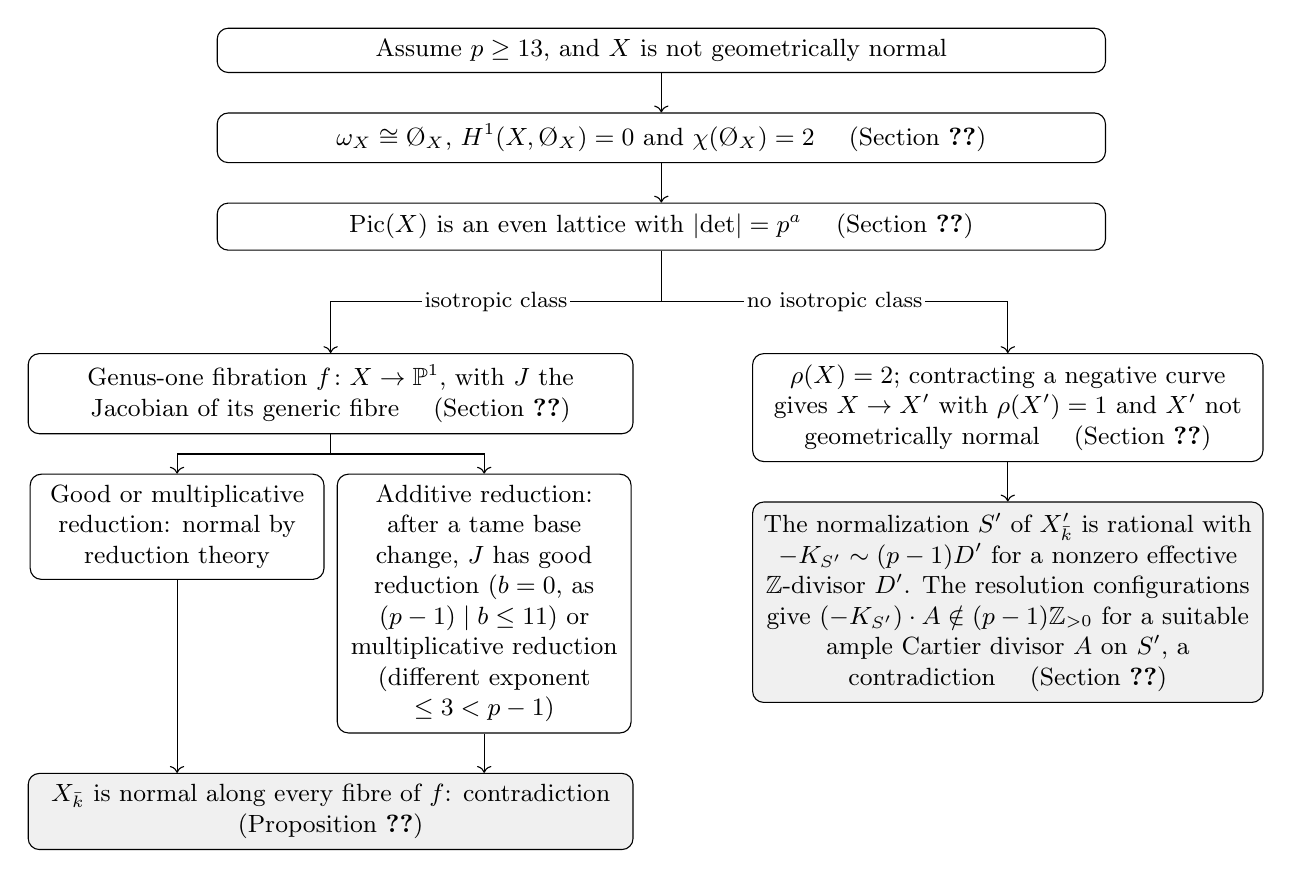
\begin{tikzpicture}[
  box/.style={draw, rounded corners, align=flush center, font=\small, inner sep=4pt},
  last/.style={box, fill=gray!12},
  lab/.style={font=\footnotesize, fill=white, inner sep=1pt},
]
\node[box, text width=11cm] (s) at (0,0) {Assume $p\geq 13$, and $X$ is not geometrically normal};
\node[box, text width=11cm, anchor=north] (a) at ([yshift=-5mm]s.south) {$\omega_X\cong\O_X$, $H^1(X,\O_X) = 0$ and $\chi(\O_X) = 2$ \quad(Section~\ref{sec:torsors})};
\node[box, text width=11cm, anchor=north] (b) at ([yshift=-5mm]a.south) {$\Pic(X)$ is an even lattice with $\lvert\det\rvert = p^a$ \quad(Section~\ref{sec:torsors})};
\node[box, text width=7.4cm, anchor=north] (c) at ([xshift=-4.2cm,yshift=-13mm]b.south) {Genus-one fibration $f\from X\to\PP^1$, with $J$ the Jacobian of its generic fibre \quad(Section~\ref{sec:genus-one})};
\node[box, text width=6.2cm, anchor=north] (d) at ([xshift=4.4cm,yshift=-13mm]b.south) {$\rho(X) = 2$; contracting a negative curve gives $X\to X'$ with $\rho(X') = 1$ and $X'$ not geometrically normal \quad(Section~\ref{sec:rank-two})};
\node[box, text width=3.45cm, anchor=north] (c1) at ([xshift=-1.95cm,yshift=-5mm]c.south) {Good or multiplicative reduction: normal by reduction theory};
\node[box, text width=3.45cm, anchor=north] (c2) at ([xshift=1.95cm,yshift=-5mm]c.south) {Additive reduction: after a tame base change, $J$ has good reduction ($b = 0$, as $(p-1)\mid b\leq 11$) or multiplicative reduction (different exponent $\leq 3<p-1$)};
\node[last, text width=7.4cm, anchor=north] (ce) at ([xshift=-1.95cm,yshift=-5mm]c2.south) {$X_{\bar k}$ is normal along every fibre of $f$: contradiction \quad(Proposition~\ref{prop:genus-one})};
\node[last, text width=6.2cm, anchor=north] (e) at ([yshift=-5mm]d.south) {The normalization $S'$ of $X'_{\bar k}$ is rational with $-K_{S'}\sim(p-1)D'$ for a nonzero effective $\ZZ$-divisor $D'$. The resolution configurations give $(-K_{S'})\cdot A\notin(p-1)\ZZ_{>0}$ for a suitable ample Cartier divisor $A$ on $S'$, a contradiction \quad(Section~\ref{sec:rank-one})};
\draw[->] (s) -- (a);
\draw[->] (a) -- (b);
\draw[->] (b.south) -- ++(0,-6.5mm) -| node[lab, pos=0.25] {isotropic class} (c.north);
\draw[->] (b.south) -- ++(0,-6.5mm) -| node[lab, pos=0.25] {no isotropic class} (d.north);
\draw[->] (c.south) -- ++(0,-2.5mm) -| (c1.north);
\draw[->] (c.south) -- ++(0,-2.5mm) -| (c2.north);
\draw[->] (c1.south) -- (c1.south |- ce.north);
\draw[->] (c2.south) -- (c2.south |- ce.north);
\draw[->] (d) -- (e);
\end{tikzpicture}
\caption{Structure of the proof of Theorem~\ref{thm:main}.}
\label{fig:strategy-main}
\end{figure}

\subsection{Proof strategy of Theorem~\ref{thm:intro-smooth}}

Assume now that $p\geq 23$.
By Theorem~\ref{thm:main}, the geometric surface $Y := X_{\bar k}$ is normal.
We may assume that $k$ is $F$-finite and separably closed.
The elliptic case is excluded by combining a local bound $d\leq 3$ on the degree of the singularity with a computer-assisted enumeration forcing $d = 4$.
The computation is needed only when $p\equiv 1\pmod 4$ and $p\leq 6912$.
Figure~\ref{fig:strategy-smooth} shows the structure of the argument.

\begin{figure}[ht]
\centering
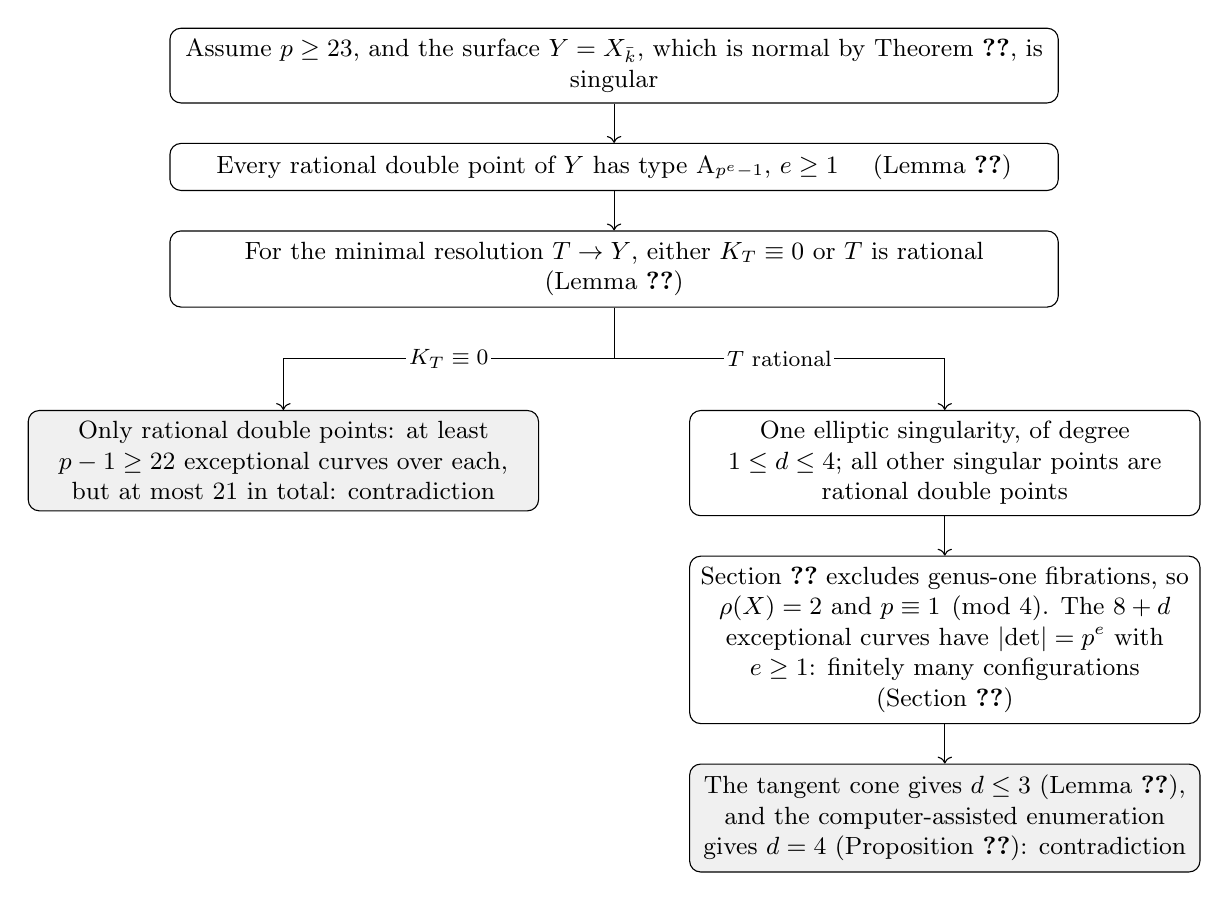
\begin{tikzpicture}[
  box/.style={draw, rounded corners, align=flush center, font=\small, inner sep=4pt},
  last/.style={box, fill=gray!12},
  lab/.style={font=\footnotesize, fill=white, inner sep=1pt},
]
\node[box, text width=11cm] (s) at (0,0) {Assume $p\geq 23$, and the surface $Y = X_{\bar k}$, which is normal by Theorem~\ref{thm:main}, is singular};
\node[box, text width=11cm, anchor=north] (a) at ([yshift=-5mm]s.south) {Every rational double point of $Y$ has type $\mathrm A_{p^e-1}$, $e\geq 1$ \quad(Lemma~\ref{lem:geometric-rdp})};
\node[box, text width=11cm, anchor=north] (b) at ([yshift=-5mm]a.south) {For the minimal resolution $T\to Y$, either $K_T\equiv 0$ or $T$ is rational \quad(Lemma~\ref{lem:smooth-structure})};
\node[last, text width=6.2cm, anchor=north] (l) at ([xshift=-4.2cm,yshift=-13mm]b.south) {Only rational double points: at least $p-1\geq 22$ exceptional curves over each, but at most $21$ in total: contradiction};
\node[box, text width=6.2cm, anchor=north] (r) at ([xshift=4.2cm,yshift=-13mm]b.south) {One elliptic singularity, of degree $1\leq d\leq 4$; all other singular points are rational double points};
\node[box, text width=6.2cm, anchor=north] (c) at ([yshift=-5mm]r.south) {Section~\ref{sec:genus-one} excludes genus-one fibrations, so $\rho(X) = 2$ and $p\equiv 1\pmod 4$. The $8+d$ exceptional curves have $\lvert\det\rvert = p^e$ with $e\geq 1$: finitely many configurations \quad(Section~\ref{sec:smooth})};
\node[last, text width=6.2cm, anchor=north] (d) at ([yshift=-5mm]c.south) {The tangent cone gives $d\leq 3$ (Lemma~\ref{lem:smooth-tangent}), and the computer-assisted enumeration gives $d = 4$ (Proposition~\ref{prop:smooth-enum}): contradiction};
\draw[->] (s) -- (a);
\draw[->] (a) -- (b);
\draw[->] (b.south) -- ++(0,-6.5mm) -| node[lab, pos=0.25] {$K_T\equiv 0$} (l.north);
\draw[->] (b.south) -- ++(0,-6.5mm) -| node[lab, pos=0.25] {$T$ rational} (r.north);
\draw[->] (r) -- (c);
\draw[->] (c) -- (d);
\end{tikzpicture}
\caption{Structure of the proof of Theorem~\ref{thm:intro-smooth}.}
\label{fig:strategy-smooth}
\end{figure}

\subsection*{Acknowledgements}
The author thanks Lei Zhang for sharing an initial draft of this work, which was generated by Jie Liu using ChatGPT.
That draft showed that the surfaces studied here are smooth for $p\geq p_0$, with an ineffective constant $p_0$.
The author improved this result with the help of Claude Code, and contributed mainly by reorganizing the exposition.

\section{Conventions and preliminaries}\label{sec:setup}
\subsection{Conventions}\label{subsec:conventions}
\begin{itemize}
\item Throughout, let $k$ be the base field, of characteristic $p>0$.
\item Surfaces and curves are integral and of finite type over $k$, unless stated otherwise.
\item For a line bundle $\mathcal L$ on a proper curve over a field $F$, we write $\deg_F(\mathcal L)$ for its degree over $F$.
  For a Cartier divisor $D$ on a surface $X$ and an integral curve $C\subset X$ proper over $F$, we put $(D\cdot C)_F := \deg_F(\O_X(D)|_C)$ and write $(D^2)_F$ for self-intersection.
  Unless indicated otherwise, intersection numbers on a surface over $F$ are computed over $F$, and intersections with vertical curves on a model over a discrete valuation ring are computed over its residue field.
  We omit the subscript when the field is clear.
\item If a curve $C$ is proper over a finite extension $\ell/k$, then $\deg_k(\mathcal L) = [\ell:k]\deg_\ell(\mathcal L)$ for every line bundle $\mathcal L$ on $C$.
  For an integral proper curve $C\subset X$ over $k$, with normalization $\nu\from C^\nu\to C$ and $\ell = H^0(C^\nu,\O_{C^\nu})$, we also write $(D\cdot C)_\ell := \deg_\ell\bigl(\nu^*(\O_X(D)|_C)\bigr)$, so
  \[
    (D\cdot C)_k = [\ell:k](D\cdot C)_\ell.
  \]
\item On a normal projective surface we use Mumford's rational intersection pairing of Weil divisors, computed over the base field of the surface.
\item We write $\sim$ for linear equivalence and $\equiv$ for numerical equivalence.
\item For a $\QQ$-factorial normal projective surface $Z$, we write $N^1(Z)_\QQ$ for the $\QQ$-vector space of Weil divisors with rational coefficients modulo numerical equivalence, and $\rho(Z) = \dim N^1(Z)_\QQ$.
\item The intersection form on $N^1(Z)_\QQ$ is \emph{isotropic} if $D^2 = 0$ for some nonzero $D\in N^1(Z)_\QQ$, and \emph{anisotropic} otherwise.
\item A \emph{negative curve} on a surface is a curve with negative self-intersection.
\item A \emph{fibration} is a proper morphism $f\from W\to B$ of schemes with $f_*\O_W = \O_B$.
\item For a scheme $W$ over $k$ and a field extension $k'/k$ we write $W_{k'} = W\times_k\Spec k'$.
\item If $W$ is geometrically integral over $k$, its \emph{geometric normalization} is the normalization of $W_{\bar k}$.
\item A locally Noetherian scheme $W$ over a field $k$ is \emph{geometrically regular} at a point $w$ if, for every finite extension $k'/k$, the scheme $W_{k'}$ is regular at every point over $w$ \cite[D\'efinition~6.7.6]{EGA}.
  If $W_{\bar k}$ is locally Noetherian, for instance if $W$ is locally of finite type over $k$, then $W$ is geometrically regular if and only if $W_{\bar k}$ is regular, by \cite[Proposition~5.13.7]{EGA} and faithfully flat descent of regularity \cite[Tag~\stackstag{07NG}]{Stacks}; cf.\ \cite[Proposition~6.7.7]{EGA}.
\item We write $F^e_W$ for the $e$-th power of the absolute Frobenius morphism of an $\FF_p$-scheme $W$.
\item For a finite surjective morphism $g\from W_1\to W_2$ of normal Noetherian integral schemes and a Weil divisor $D$ on $W_2$, the pullback $g^*D$ is defined as the closure of the pullback of $D$ restricted to the regular locus of $W_2$; the complement of the regular locus has codimension at least two, and so does its preimage.
This pullback is compatible with composition, because this may be checked at points of codimension one, where all Weil divisors are Cartier.
\item For a local ring $(R,\mathfrak m,\kappa)$, we write $\widehat R$ for its $\mathfrak m$-adic completion.
\item
  For a point $z$ of a scheme $Z$, we write $\O^{\rm sh}_{Z,z}$ for the \emph{strict henselization} of $\O_{Z,z}$ with respect to a separable closure of $\kappa(z)$.
  The ring $\O^{\rm sh}_{Z,z}$ is a filtered colimit of \'etale $\O_{Z,z}$-algebras, and the map $\O_{Z,z}\to\O^{\rm sh}_{Z,z}$ is flat and local \cite[Tag~\stackstag{03QL}]{Stacks}.
\end{itemize}

\subsection{Purely inseparable base change}\label{subsec:canonical-base-change}
We record the behavior of canonical divisors under base change; cf.\ \cite{Tan18BC} and \cite[Theorems~1.1 and~1.2]{PW22}.
For our application, we need the case where the scheme $X/k$ is not necessarily of finite type, which is due to \cite{NT24}. For simplicity, we only consider the case where $X$ is geometrically integral.
\begin{lemma}\label{lem:canonical-base-change}
Let $A$ be an excellent Gorenstein Noetherian $k$-algebra of finite Krull dimension.
Let $X\to\Spec A$ be a flat Gorenstein morphism of finite type, with $X$ normal and geometrically integral over $k$.
For a finite field extension $k'/k$, put $A' = A\otimes_k k'$ and $X_{A'} = X\times_A\Spec A'$.
Let $\nu\from X'\to X_{A'}$ be the normalization of the integral scheme $X_{A'} = X_{k'}$.
Then the divisorial conductor of $\nu$ is $(p-1)C_{k'}$ for an effective integral Weil divisor $C_{k'}$, and
\begin{equation}\label{eq:canonical-base-change}
  \omega_{X'/A'}\cong\O_{X'}\bigl(-(p-1)C_{k'}\bigr)\otimes\nu^*\omega_{X_{A'}/A'},
\end{equation}
where $\omega_{X'/A'}$ denotes the relative canonical sheaf, a rank-one reflexive sheaf, and $C_{k'} = 0$ if and only if $X_{A'}$ is normal.
\end{lemma}

\begin{proof}
The normalization $\nu$ is finite since $A$ is excellent.
The ring $A'$ is Gorenstein by base change, and $X_{A'}$ is Gorenstein because $X_{A'}\to\Spec A'$ is Gorenstein \cite[Tags~\stackstag{0C03} and~\stackstag{0BJL}]{Stacks}.
Since $X$ is of finite type over the excellent ring $A$, it is Noetherian and Japanese, so \cite[Corollary~5.10]{NT24} shows that the divisorial conductor of $\nu$ is $(p-1)C_{k'}$ for an effective integral Weil divisor $C_{k'}$.
Since $\omega_{X_{A'}/A'}$ is invertible, finite duality gives \eqref{eq:canonical-base-change} in codimension one, and both sides are reflexive on $X'$, so the isomorphism extends globally.
Finally, $C_{k'} = 0$ precisely when $X_{A'}$ is normal in codimension one; since $X_{A'}$ is Gorenstein and hence $S_2$, this is equivalent to normality by Serre's criterion.
\end{proof}

For extensions of height one, the vanishing of this conductor divisor admits the following local criterion, which can be seen as an algebraic version of Ji--Waldron's description of normalized base changes by foliations \cite[Sections~3 and~4]{JW21}.
\begin{lemma}\label{lem:normality-derivation}
Let $A$ be a normal $k$-domain, and let $k'/k$ be finite with $k'^p\subseteq k$.
Suppose that $B := A\otimes_k k'$ is a domain, with normalization $\widetilde B$.
For $D\in\Der_k(k')$, write $D_B = \mathrm{id}_A\otimes D$ and use the same notation for its extension to $\Frac(B)$.
Then $B$ is normal if and only if $D_B$ preserves $\widetilde B$ for every $D\in\Der_k(k')$.
\end{lemma}

\begin{proof}
The forward implication is immediate.
For the converse, put $L = \Frac(A)$ and $K = L\otimes_k k' = \Frac(B)$.
Choose a $p$-basis $\gamma_1,\ldots,\gamma_r$ of $k'/k$ and let $\delta_i$ be the $L$-derivation of $K$ with $\delta_i(\gamma_j) = \delta_{ij}$.
The commuting derivations $\delta_i$ satisfy $\delta_i^p = 0$ and preserve $\widetilde B$ by hypothesis.
They therefore define an action of $G = \alpha_p^r$ on $\Spec\widetilde B$ \cite[Section~4]{ST23}.
Writing $t_1,\ldots,t_r$ for the coordinates on $G$, its coaction on $k'$ sends $\gamma_i$ to $\gamma_i+t_i$, so the inclusion $k'\hookrightarrow\widetilde B$ is equivariant.
Since $\Spec k'\to\Spec k$ is a $G$-torsor, faithfully flat descent for algebras gives
\[
  \widetilde B\cong (\widetilde B)^G\otimes_k k'.
\]
The common kernel of the $\delta_i$ in $K$ is $L$, so $(\widetilde B)^G = \widetilde B\cap L$.
Every element of this intersection is integral over $A$, since $B$ is integral over $A$.
Normality of $A$ therefore gives $(\widetilde B)^G = A$, and the displayed isomorphism is the natural map $B\to\widetilde B$.
Hence $B$ is normal.
\end{proof}


\subsection{Killing a cohomology class by a generic $\alpha_p$-torsor}\label{subsec:generic-alpha-p-torsor}
\begin{lemma}\label{lem:generic-alpha-p-torsor}
Let $X/k$ be a regular projective geometrically integral variety with $H^1(X,\O_X)\neq 0$.
Suppose that $H^1((X_{k^{1/p^e}})^\nu,\O) = 0$ for some $e\geq 1$.
Then over $K = k(a)$, with $a$ transcendental over $k$, there is an $\alpha_p$-torsor $\pi\from V\to X_K$, where $V$ is a regular projective geometrically non-reduced variety with $H^0(V,\O_V) = K$ and $\omega_V\cong\pi^*\omega_{X_K}$.
\end{lemma}

\begin{proof}
Put $\ell = k^{1/p^e}$ and $T = (X_\ell)^\nu$.
Then $H^0(T,\O_T) = \ell$.
The absolute Frobenius $F_X^e$ factors through $T\to X$.
Since $H^1(T,\O_T) = 0$, we have $(F_X^*)^e = 0$ on $H^1(X,\O_X)$.
Choose $\eta\neq 0$ in $H^1(X,\O_X)$ and let $r\geq 1$ be minimal with $(F_X^*)^r\eta = 0$.
Then $\xi := (F_X^*)^{r-1}\eta$ is nonzero and satisfies $F_X^*(\xi) = 0$.
Choose a finite affine open cover $\{U_i = \Spec A_i\}$ and a \v{C}ech cocycle $(g_{ij})$ representing $\xi$.
Since $F_X^*(\xi) = 0$, the cocycle $(g_{ij}^p)$ is a coboundary, so there are $f_i\in A_i$ with $g_{ij}^p = f_i-f_j$.
Write $\xi_K = \xi\otimes 1\in H^1(X_K,\O_{X_K})$.

Glue
\[
  V_i = \Spec\bigl((A_i\otimes_kK)[t_i]/(t_i^p-f_i-a)\bigr)
\]
by $t_i = t_j+g_{ij}$.
These transitions preserve the equations because $g_{ij}^p = f_i-f_j$, and they satisfy the cocycle condition.
Translations $t_i\mapsto t_i+\varepsilon$ define an $\alpha_p$-torsor $\pi\from V\to X_K$.
Since $g_{ij} = t_i-t_j$ on $V$, we have $\pi^*\xi_K = 0$ in $H^1(V,\O_V)$.
Each $V_i$ is regular, since its coordinate ring is a localization of the regular ring
\[
  A_i[a,t_i]/(t_i^p-f_i-a)\cong A_i[t_i].
\]
Hence $V$ is regular.
Since $\pi$ is a universal homeomorphism and $X_K$ is integral, $V$ is integral.
The morphism $\pi$ is finite, so $V$ is projective over $K$.

To show that $H^0(V,\O_V) = K$, let $s\in H^0(V,\O_V)$ be nonzero, and represent $s|_{V_i}$ by a polynomial $s_i(t_i)\in (A_i\otimes_kK)[t_i]$ of degree $<p$.
The transitions preserve degree, so let $m$ be the common degree of the $s_i$.
Their leading coefficients glue to an element $b\in H^0(X_K,\O_{X_K}) = K$.
If $m>0$, write their two leading terms as $bt_i^m+c_it_i^{m-1}$, where $b\in K^\times$ and $c_i\in A_i\otimes_kK$.
Comparing coefficients of $t_j^{m-1}$ in $s_i(t_j+g_{ij}) = s_j(t_j)$ gives $c_j-c_i = mbg_{ij}$, so $mb\xi_K = 0$ in $H^1(X_K,\O_{X_K})$.
This contradicts $\xi_K\neq 0$.
Thus the $s_i$ have degree zero and glue to an element of $K$, so $H^0(V,\O_V) = K$.

Let $W_i$ be the inverse image of $U_i$ under $T\to X$.
Since $H^1(T,\O_T) = 0$, the pulled-back cocycle has the form $g_{ij} = h_i-h_j$ with $h_i\in H^0(W_i,\O_T)$.
The functions $f_i-h_i^p$ glue to a constant $\lambda\in H^0(T,\mathcal O_T) = \ell$.
Put $L = \ell(a)$ and $T_L = T\times_\ell L$.
Consider the Cartesian square
\[
  \begin{array}{ccc}
    V\times_{X_K}T_L &\longrightarrow& V\\
    \downarrow &&\downarrow\pi\\
    T_L &\longrightarrow& X_K.
  \end{array}
\]
The coordinates $z_i = t_i-h_i$ give an isomorphism
\[
  V\times_{X_K}T_L\cong T_L\times_L\Spec L[z]/(z^p-a-\lambda).
\]
Put $L' = L((a+\lambda)^{1/p})$ and $T_{L'} = T\times_\ell L'$.
Then the projection $V\times_{X_K}T_{L'}\to T_{L'}$ is a trivial $\alpha_p$-torsor.
Since $T_{L'}\to X_{L'}$ is birational, $V_{L'}$ is generically nonreduced.
Hence $V$ is not geometrically reduced over $K$.

Put $B_i = H^0(V_i,\O_{V_i})$.
Let $\varphi_i\from B_i\to A_i\otimes_kK$ be the coefficient functional $\sum_{r<p}b_rt_i^r\mapsto b_{p-1}$.
For $0\leq r<p$, the multiple $t_i^{p-1-r}\varphi_i$ extracts the coefficient of $t_i^r$.
These multiples form the dual basis to $1,t_i,\ldots,t_i^{p-1}$, so $\varphi_i$ generates $\operatorname{Hom}_{A_i\otimes_kK}(B_i,A_i\otimes_kK)$ as a $B_i$-module.
The translations $t_i = t_j+g_{ij}$ preserve the coefficient of degree $p-1$, so these generators glue to trivialize $\omega_{V/X_K}$.
Finite duality then gives $\omega_V\cong\pi^*\omega_{X_K}$.
\end{proof}

\subsection{Tangent cones}\label{subsec:tangent-cones}
Let $X$ be a variety over $k$, let $x\in X$ be a closed point at which $X$ is regular, with $\kappa(x)$ purely inseparable over $k$, and let $\bar x\in X_{\bar k}$ be the geometric point over $x$.
Let $\mathfrak m_{\bar x}$ be the maximal ideal of $\O_{X_{\bar k},\bar x}$, and let $T = (\mathfrak m_{\bar x}/\mathfrak m_{\bar x}^2)^\vee$ be the Zariski tangent space of $X_{\bar k}$ at $\bar x$.
Write $C = \Spec\bigl(\bigoplus_{j\geq 0}\mathfrak m_{\bar x}^j/\mathfrak m_{\bar x}^{j+1}\bigr)\subseteq T$ for the tangent cone and $I_C$ for its homogeneous ideal.
The tangent cone $C$ has the same dimension as $X$, and $C = T$ if $\bar x$ is regular.
If $\bar x$ is a singular point, let $e$ be the lowest degree of a nonzero form in $I_C$.
We define the space of \emph{vertical directions} to be
\[
  L = \{v\in T : v(f) = 0\text{ for all }f\in\mathfrak m_x\},
\]
where $\mathfrak m_x$ is the maximal ideal of $\O_{X,x}$, mapped to $\mathfrak m_{\bar x}/\mathfrak m_{\bar x}^2$ by the projection $\pi\from X_{\bar k}\to X$.
Equivalently, $L$ is the Zariski tangent space at $\bar x$ of the one-point fibre $\pi^{-1}(x) = \Spec(\kappa(x)\otimes_k\overline k)$.

\begin{lemma}\label{lem:tangent-cone}
In this situation, the following hold.
\begin{enumerate}[label=\textup{(\arabic*)}]
\item $\dim L = \dim_{\kappa(x)}\Omega_{\kappa(x)/k}$ and $\dim T\leq\dim X+\dim L$; in particular, $\dim T\leq\dim X+1$ if $\kappa(x)/k$ is simple.
\item If $y_1,\dots,y_N$ is a basis of $\mathfrak m_{\bar x}/\mathfrak m_{\bar x}^2$ such that $y_1,\dots,y_u$ span the image of $\mathfrak m_x$, so that $L = \{v\in T : v(y_1) = \dots = v(y_u) = 0\}$, then $I_C$ is stable under $\partial/\partial y_j$ for $j>u$.
\item Suppose that $e<p$, and let $y_1,\dots,y_N$ be as in \textup{(2)}.
  Then every form of degree $e$ in $I_C$ is a polynomial in $y_1,\dots,y_u$ alone, so it does not involve the coordinates along $L$.
  In particular, if $I_C$ is generated by one form, then $C$ is the preimage of a cone in $T/L$ under the projection $T\to T/L$.
\end{enumerate}
\end{lemma}

\begin{proof}
Put $\kappa = \kappa(x)$.
For (1), the description of $L$ as the tangent space of the fibre gives $L^\vee\cong\Omega_{\kappa/k}\otimes_\kappa\bar k$.
Since $\mathfrak m_x$ is generated by $\dim X$ elements and $L$ is the annihilator of its image in the cotangent space, $\dim T-\dim L\leq\dim X$.

For (2), put $A = \O_{X,x}$ and $B = A\otimes_k\kappa$.
The ring $B$ is finite over $A$, and $B/\mathfrak m_xB = \kappa\otimes_k\kappa$ is local with residue field $\kappa$ because $\kappa/k$ is purely inseparable.
Hence $B$ is local with residue field $\kappa$, and it is the local ring of $X_\kappa$ at the unique point over $x$, which is $\kappa$-rational.
Let $\mathfrak m$ be the maximal ideal of $B$, let $\Sigma\subseteq\mathfrak m/\mathfrak m^2$ be the $\kappa$-span of the image of $\mathfrak m_x$, and write the associated graded ring $\operatorname{gr}_{\mathfrak m}B$ as $S/I^*$ with $S = \Sym_\kappa(\mathfrak m/\mathfrak m^2)$, where $I^*$ is the ideal of initial forms.
The maximal ideal of $\O_{X_{\bar k},\bar x}$ is generated by $\mathfrak m$, and $\operatorname{gr}_{\mathfrak m_{\bar x}}\O_{X_{\bar k},\bar x} = \operatorname{gr}_{\mathfrak m}B\otimes_\kappa\overline k$.
Hence $T = (\mathfrak m/\mathfrak m^2)^\vee\otimes_\kappa\overline k$, $I_C = I^*\otimes_\kappa\overline k$, and $L$ is the annihilator of $\Sigma$.

For $b\in\kappa$ with a lift $\tilde b\in A$, put $w_b = \tilde b\otimes 1-1\otimes b$, which lies in $\mathfrak m$.
Let $\delta\in\Der_k(\kappa)$.
Then $D = \mathrm{id}_A\otimes\delta$ is a derivation of $B$ which vanishes on $\mathfrak m_x$ and satisfies $D(w_b) = -1\otimes\delta(b)$, so $D(\mathfrak m^j)\subseteq\mathfrak m^{j-1}$ for $j\geq 1$.
The induced maps $\mathfrak m^j/\mathfrak m^{j+1}\to\mathfrak m^{j-1}/\mathfrak m^j$ form a derivation of degree $-1$ of $S/I^*$, which is $\kappa$-linear because $f\,D(1\otimes c)\in\mathfrak m^j$ for $f\in\mathfrak m^j$ and $c\in\kappa$.
Hence it is induced by the $\kappa$-linear derivation $\partial_\lambda$ of $S$ with $\partial_\lambda(y) = \lambda(y)$ for $y\in\mathfrak m/\mathfrak m^2$, where $\lambda$ is the functional $f\mapsto D(f)\bmod\mathfrak m$ on $\mathfrak m/\mathfrak m^2$, and therefore $\partial_\lambda(I^*)\subseteq I^*$.
The functional $\lambda$ vanishes on $\Sigma$, and $\lambda(w_b) = -\delta(b)$.

The cotangent-space identification for the fibre $\Spec(\kappa\otimes_k\kappa)$ gives an isomorphism $\Omega_{\kappa/k}\cong(\mathfrak m/\mathfrak m^2)/\Sigma$, sending $db$ to the class of $w_b$.
Under this identification, $\lambda$ corresponds to $-\delta$, so these functionals exhaust the dual of $(\mathfrak m/\mathfrak m^2)/\Sigma$ as $\delta$ varies.
Thus $I^*$ is stable under $\partial_\lambda$ for every functional $\lambda$ on $\mathfrak m/\mathfrak m^2$ vanishing on $\Sigma$.

Choose a basis $y_1,\dots,y_N$ of $\mathfrak m/\mathfrak m^2$ such that $y_1,\dots,y_u$ span $\Sigma$.
Then $L = \{v\in T : v(y_1) = \dots = v(y_u) = 0\}$, and $I^*$ is stable under $\partial/\partial y_j$ for $j>u$.
The derivations $\partial/\partial y_j$ with $j>u$ are the derivatives along a basis of $L$, so this condition does not depend on the choice of coordinates.

For (3), let $Q\in I^*$ be homogeneous of degree $e<p$.
For $j>u$ we have $\partial Q/\partial y_j\in I^*_{e-1} = 0$, and every exponent occurring in $Q$ is at most $e<p$, so $Q$ is a polynomial in $y_1,\dots,y_u$.
The forms of degree $e$ in $I_C$ are the $\overline k$-linear combinations of such $Q$, and $\overline k[y_1,\dots,y_u]$ is the coordinate ring of $T/L$ for every choice of coordinates as in (2), which proves the first assertion of (3).
If $I_C$ is generated by one form, then this form has degree $e$, so $C$ is the preimage of the cone in $T/L$ defined by the same form.
\end{proof}


\subsection{Birational contractions}\label{subsec:birational-surfaces}
% Let $\varepsilon\from Y'\to Y$ be the blowup of a codimension-two closed point $P$ on a regular Noetherian integral scheme $Y$ of dimension two, with exceptional curve $E$.
% Then $Y'$ is regular, $E\cong\PP^1_{\kappa(P)}$ and $\O_E(E)\cong\O_{\PP^1_{\kappa(P)}}(-1)$ \cite[Tags~\stackstag{0AGQ} and~\stackstag{0AGR}]{Stacks}.
% If $Y$ admits a dualizing sheaf $\omega_Y$, adjunction gives the induced dualizing sheaf on $Y'$ as
% \begin{equation}\label{eq:blowup-canonical}
%   \omega_{Y'}\cong\varepsilon^*\omega_Y\otimes\O_{Y'}(E).
% \end{equation}
% The same formula holds for the relative dualizing sheaves of regular flat models of curves over a discrete valuation ring.
% If $Y$ is a projective surface over $k$, then, with compatible canonical divisors,
% \begin{equation}\label{eq:blowup-intersections}
%   K_{Y'} = \varepsilon^*K_Y+E,\qquad
%   (K_{Y'}\cdot E)_k = (E^2)_k = -[\kappa(P):k],\qquad
%   (K_{Y'}^2)_k = (K_Y^2)_k-[\kappa(P):k].
% \end{equation}
% Moreover, if $-K_{Y'}$ is nef, then $-K_Y$ is nef: for a curve $C\subset Y$ with strict transform $\widetilde C$, the projection formula gives
% \[
%   -K_Y\cdot C = (-K_{Y'}+E)\cdot\widetilde C\geq 0.
% \]

% Let $\mu\from T\to S$ be the minimal resolution of a normal projective surface over an algebraically closed field.
% Choose canonical divisors with $\mu_*K_T = K_S$.
% Minimality makes $K_T$ relatively nef by \cite[Theorem~10.5]{Kol13}, and the negative definite exceptional intersection matrix gives
% \begin{equation}\label{eq:minimal-resolution-canonical}
%   K_T = \mu^*K_S-Z,\qquad Z\geq 0,
% \end{equation}
% with $Z$ an exceptional $\QQ$-divisor \cite[Claim~10.3.5]{Kol13}.
% Here $\mu^*K_S$ is Mumford's numerical pullback, characterized by $\mu_*(\mu^*K_S) = K_S$ and $(\mu^*K_S)\cdot E = 0$ for every exceptional curve $E$.
% If $K_S$ is Cartier, then this is the ordinary pullback and $Z$ is integral.

\begin{definition}\label{def:minus-one-curve}
Let $X$ be a regular integral scheme of dimension two, proper and flat over $S$, where $S$ is either the spectrum of a field or a Dedekind scheme of dimension one.
A \emph{vertical curve} on $X$ is an integral closed subscheme $C\subset X$ of dimension one contained in a fibre $X_s$ over a closed point $s\in S$.
We call such a curve $C$ a \emph{$(-1)$-curve} if
\[
  (K_{X/S}\cdot C)_{k_C} = (C^2)_{k_C} = -1,
\]
where $K_{X/S}$ is a relative canonical divisor and $k_C = H^0(C,\O_C)$.
For such a curve $C$, adjunction gives $H^1(C,\O_C) = 0$.
By Castelnuovo's criterion \cite[Theorem~9.3.8 and Proposition~9.3.10]{Liu02}, these are exactly the vertical curves that can be contracted to a regular point.
\end{definition}

We record standard facts about contracting negative curves, including the residue-field details needed below.

\begin{lemma}\label{lem:contraction}
Let $k$ be a separably closed field of characteristic $p>3$, and let $X$ be a regular projective surface over $k$ with $K_X\equiv 0$.
Let $C\subset X$ be a negative curve, and put $\ell = H^0(C,\O_C)$.
\begin{enumerate}
\item $C\cong\PP^1_\ell$, $(C^2)_\ell = -2$, and $\O_C(C)\cong\O_{\PP^1_\ell}(-2)$.
\item There is a birational morphism $f\from X\to X'$ onto a normal projective surface which contracts exactly $C$, to a point $P$ with $\kappa(P) = \ell$.
  Moreover $R^1f_*\O_X = 0$ and $\rho(X') = \rho(X)-1$.
\item The surface $X'$ is Gorenstein, and $f^*\omega_{X'}\cong\omega_X$.
\item $2D$ is Cartier for every Weil divisor $D$ on $X'$.
\item There is an isomorphism of rings $\widehat\O_{X',P}\cong \ell[[u,v,w]]/(uv-w^2)$; in particular $X'$ is a local complete intersection over $k$.
  \textup{(}This isomorphism need not be an isomorphism of $k$-algebras.\textup{)}
\end{enumerate}
\end{lemma}

\begin{proof}
(1) The curve $C$ is a Cartier divisor on the regular surface $X$, hence Gorenstein.
Put $g = \dim_\ell H^1(C,\O_C)$.
Adjunction gives
\[
  (C^2)_\ell = ((K_X+C)\cdot C)_\ell = 2(g-1)<0,
\]
so $g = 0$ and $(C^2)_\ell = -2$.
By \cite[Lemma~10.6(3)]{Kol13}, $C$ is a conic or $\PP^1$ over $\ell$.
Since $\ell$ is separably closed and $p\neq 2$, an integral conic over $\ell$ is smooth and split, so $C\cong\PP^1_\ell$.
The normal bundle has degree $(C^2)_\ell = -2$, hence is $\O_{\PP^1_\ell}(-2)$, proving (1).

(2) The negative curve $C$ spans a $(K_X+C)$-negative extremal ray.
Applying \cite[Theorem~4.4]{Tan18} with boundary $C$ gives a projective birational morphism $f\from X\to X'$ contracting exactly $C$, with $X'$ normal and projective and $\rho(X') = \rho(X)-1$.
Since $K_X\cdot C = 0$ and $-C$ is $f$-nef, \cite[Theorem~10.4]{Kol13} gives $R^1f_*\O_X(-jC) = 0$ for every $j\geq 0$.
Thus $P$ is a rational singularity, and \cite[Proposition~10.9(4)]{Kol13} gives $\kappa(P) = \ell$.

(3) The numerical discrepancy of $C$ is zero because $K_X\cdot C = 0$.
Hence $X'$ is Gorenstein and $f$ is crepant by \cite[Theorem~2.29(2)]{Kol13}.

(4) The intersection matrix over $\ell$ is $(-2)$, so \cite[Proposition~10.9(3)]{Kol13} shows that $2D$ is Cartier at $P$ for every Weil divisor $D$ on $X'$.
Since $X'$ is regular away from $P$, the divisor $2D$ is Cartier everywhere.

(5) Put $R = \O_{X',P}$ and $I_j = (f_*\O_X(-jC))_P$.
Pushing forward $0\to\O_X(-C)\to\O_X\to\O_C\to0$ and taking the stalk at $P$ gives $I_1 = \ker(R\to H^0(C,\O_C)=\kappa(P)) = \mathfrak m_P$.
Similarly, since $R^1f_*\O_X(-jC) = 0$ for all $j\geq 0$, we have $I_j/I_{j+1}\cong H^0(\PP^1_\ell,\O(2j))$, compatibly with multiplication.
The multiplication map $H^0(\PP^1_\ell,\O(2))^{\otimes_\ell j}\to H^0(\PP^1_\ell,\O(2j))$ is surjective, since every monomial of degree $2j$ is a product of $j$ quadratic monomials.
Hence every class in $I_j/I_{j+1}$ is a sum of products of $j$ classes from $I_1/I_2$, so $I_j = I_1^j+I_{j+1} = \mathfrak m_P^j+I_{j+1}$.
Iterating this equality gives $I_j = \mathfrak m_P^j+I_n$ for all $n\geq j$.
By formal functions, $\widehat R\cong\varprojlim_n R/I_n$; taking limits gives $I_j\widehat R = \mathfrak m_P^j\widehat R$ and hence
\[
  \operatorname{gr}_{\mathfrak m_P}\widehat R
  \cong \bigoplus_{j\geq 0}H^0(\PP^1_\ell,\O(2j))
  \cong \ell[u,v,w]/(uv-w^2).
\]
The displayed graded ring gives $\length_R(R/\mathfrak m_P^n) = \sum_{j=0}^{n-1}(2j+1) = n^2$ for $n\geq 1$.
After choosing a coefficient field identified with $\ell$, \cite[Lemma~23.4]{Lip69} therefore gives a quadratic hypersurface presentation $\widehat R\cong\ell[[u,v,w]]/(g)$.
Comparing associated graded rings, we may choose the variables $u,v,w$ and rescale $g$ so that $g-(uv-w^2)\in(u,v,w)^3$.
Since $p\neq 2$, the quadratic form $uv-w^2$ is nondegenerate.
The formal Morse lemma \cite[Lemma~10.43]{Kol23}, applied with coefficient ring $\ell$ and maximal ideal $(0)$, therefore gives $\widehat R\cong\ell[[u,v,w]]/(uv-w^2)$ as rings.
The hypersurface presentation and regularity of $X'$ away from $P$ imply that $X'$ is a local complete intersection over $k$ \cite[Tag~\stackstag{09Q6}]{Stacks}.
\end{proof}


\subsection{Even lattices}\label{subsec:even-lattices}
An \emph{integral lattice} is a finitely generated free abelian group $N$ equipped with a nondegenerate symmetric bilinear pairing $(\ ,\ )\from N\times N\to\ZZ$.
It is \emph{even} if $(v,v)\in 2\ZZ$ for every $v\in N$.
For a $\ZZ$-basis $e_1,\ldots,e_r$ of $N$, the matrix $G = ((e_i,e_j))_{1\leq i,j\leq r}$ is called a \emph{Gram matrix} of $N$.
Its determinant $\det N := \det G$, called the \emph{Gram determinant}, is independent of the chosen $\ZZ$-basis.
The lattice $N$ is \emph{unimodular} if $\lvert\det N\rvert = 1$, equivalently if the pairing induces an isomorphism $N\cong\Hom_\ZZ(N,\ZZ)$.
For a lattice over $\ZZ_\ell$, unimodularity means that its Gram determinant is a unit in $\ZZ_\ell$.
The pairing induces a quadratic form $q(v) = (v,v)$ on $N\otimes\QQ$.
An nonzero element $v\in N\otimes\QQ$ is called \emph{anisotropic} if $q(v)\neq 0$, and \emph{isotropic} if $q(v) = 0$.
The quadratic form $q$ (or the corresponding pairing) is called \emph{anisotropic} if it has no isotropic elements, and \emph{isotropic} otherwise. %ref: ~/math/students/Merkurev/QuadForm



\begin{lemma}\label{lem:lattice-dichotomy}
Let $p$ be an odd prime and let $N$ be an even integral lattice of signature $(1,r-1)$ with $\lvert\det N\rvert = p^a$ for an integer $a\geq 0$.
Then $r$ is even, and $N\otimes\QQ$ is anisotropic if and only if $r = 2$ and $a$ is odd.
In this case $p\equiv 1\pmod 4$.
\end{lemma}

\begin{proof}
Since $N$ is even of odd determinant, the induced bilinear form on $N/2N$ with values in $\FF_2$ is nondegenerate and alternating, so $r$ is even.
In particularly, $r\ge2$.
Then the quadratic form on $N\otimes\QQ$ is indefinite by the signature.
If $r\geq 5$, then this implies that the form is isotropic by Meyer's theorem \cite[Chapter~IV, Section~3.2, Corollary~2 to Theorem~8]{Ser73}.

Suppose that $r = 4$.
By the Hasse--Minkowski theorem \cite[Chapter~IV, Section~3.2, Theorem~8]{Ser73}, to show that $N\otimes\QQ$ is isotropic, it suffices to show that $N\otimes\RR$ is isotropic and that $N\otimes\QQ_\ell$ is isotropic for every prime $\ell$.

At $\ell = 2$, $\det N$ is a unit in $\ZZ_2$ because $\lvert\det N\rvert = p^a$ and $p$ is odd, so $N\otimes\ZZ_2$ is \emph{unimodular}.
Since it is also even, it is an orthogonal sum of two binary lattices with Gram matrices \cite[Hilfssatz~5]{Cas62}
\[
  B_1 = \begin{pmatrix}2a_1&1\\1&2b_1\end{pmatrix},\qquad
  B_2 = \begin{pmatrix}2a_2&1\\1&2b_2\end{pmatrix},
\]
where $a_1,b_1,a_2,b_2\in\ZZ_2$.
Since $\det B_1\equiv\det B_2\equiv -1\pmod 4$ and squares of $2$-adic units are $1$ modulo $4$, we have $\det N\equiv 1\pmod 4$.
Since $\det N = -p^a$, we get $p\equiv -1\pmod 4$ and that $a$ is odd.
In these coordinates, the quadratic form satisfies $q = 2Q$, where
\[
  Q(x_1,x_2,x_3,x_4) = a_1x_1^2+x_1x_2+b_1x_2^2+a_2x_3^2+x_3x_4+b_2x_4^2.
\]
The polynomial $Q$ has coefficients in $\ZZ_2$ and has the same zeros as $q$ over $\QQ_2$.
The values of $Q$ at $(1,0,0,0)$, $(0,0,1,0)$ and $(1,0,1,0)$ are $a_1$, $a_2$ and $a_1+a_2$, respectively.
So modulo $2$, the form $Q$ has a zero at one of these points.
The gradient of $Q$ modulo $2$ is $(x_2,x_1,x_4,x_3)$, so this zero is nonsingular and lifts by Hensel's lemma to a nonzero isotropic vector over $\QQ_2$.

At the real place, $N\otimes\RR$ has signature $(1,3)$ and is therefore isotropic.
At an odd prime $\ell\neq p$, the determinant is a unit in $\ZZ_\ell$, so the reduction of the lattice is a nondegenerate quaternary form over $\FF_\ell$.
Since $\ell$ is odd, \cite[Chapter~IV, Section~1.4, Theorem~1]{Ser73} gives coordinates in which this reduction is $\bar q = \sum_{i=1}^4 c_ix_i^2$ with $c_i\in\FF_\ell^\times$.
The sets $\{c_1x^2:x\in\FF_\ell\}$ and $\{-c_3-c_2y^2:y\in\FF_\ell\}$ each have $(\ell+1)/2$ elements, so they intersect.
Thus $\bar q(x,y,1,0) = 0$ for some $x,y\in\FF_\ell$, and the partial derivative with respect to $x_3$ at this zero is $2c_3\neq 0$.
Hensel's lemma therefore lifts this zero to a nonzero isotropic vector over $\QQ_\ell$.
At $\ell = p$, an anisotropic quaternary quadratic form has square discriminant \cite[Chapter~IV, Section~2.2, Theorem~6(iii)]{Ser73}, whereas $\det N$ has $p$-adic valuation $a$, which is odd, a contradiction.

Suppose $r = 2$.
Choose an orthogonal basis of $N\otimes\QQ$ and write $q(x,y) = ux^2+vy^2$ with $u,v\in\QQ^\times$.
A nonzero zero must have $y\neq 0$, and $q(x,y) = 0$ is then equivalent to $(x/y)^2 = -v/u$.
Thus $N\otimes\QQ$ is isotropic if and only if $-v/u$ is a rational square, or equivalently if $-uv$ is a rational square.
A change of basis multiplies the Gram determinant by a rational square, so $uv$ and $\det N$ have the same square class, and the criterion is equivalent to $-\det N$ being a rational square.
The signature $(1,1)$ gives $\det N<0$, so $-\det N = p^a$ is a rational square if and only if $a$ is even.
Therefore, under the assumption that $N \otimes \mathbb Q$ is anisotropic, $a$ is odd.
Since $N$ is even, its Gram matrix in an integral basis has the form $\begin{pmatrix}2b&c\\c&2d\end{pmatrix}$ with $b,c,d\in\ZZ$.
Its determinant $4bd-c^2$ is odd, so $c$ is odd and $\det N\equiv -1\pmod 4$.
Since $\det N = -p^a$, this gives $p^a\equiv 1\pmod 4$.
As $a$ is odd, $p^a\equiv p\pmod 4$, hence $p\equiv 1\pmod 4$.
\end{proof}


\subsection{Genus-one fibrations}
\begin{lemma}\label{lem:fibration}
Let $X$ be a regular projective surface over $k$ with $H^0(X,\O_X) = k$, $K_X\equiv 0$ and $\chi(\O_X) = 2$.
If the intersection form on $N^1(X)_\QQ$ is isotropic, then there is a fibration $f\from X\to B$ onto a regular projective curve.
\end{lemma}

\begin{proof}
Choose an ample divisor $A$ and a divisor $D$ with $D^2 = 0$ and $A\cdot D>0$.
Riemann--Roch gives $h^0(D)+h^0(K_X-D)\geq\chi(\O_X(D)) = \chi(\mathcal O_X) = 2$.
Hence $h^0(D)\geq 2$.

Suppose that $D$ is not nef, and let $C$ be a curve with $D\cdot C<0$.
Then $C$ is a component of every member of $\lvert D\rvert$, so $C^2<0$.
As in the proof of Lemma~\ref{lem:contraction}(1), with $h = [H^0(C,\O_C):k]$ we have $(C^2)_k = -2h$, and $(D\cdot C)_k\in h\ZZ$.
Hence $r_C(D) := D+\frac{(D\cdot C)_k}{h}C$ is a $\ZZ$-divisor with $(r_C(D)^2)_k = 0$.
The reflection $r_C$ is an isometry of $N^1(X)_\QQ$ preserving the component of the positive cone containing $A$; hence $A\cdot r_C(D)>0$, while $A\cdot r_C(D)<A\cdot D$.
By Riemann--Roch again, $h^0(r_C(D))\geq 2$.
Since the positive integer $A\cdot D$ decreases, after finitely many reflections we obtain a nef divisor $D$ with $D^2 = 0$ and $h^0(D)\geq 2$.

It follows that $\kappa(X,D) = 1$, so the nef divisor $D$ is semiample (cf.\ \cite[Lemma~2.7]{Tan20}).
The Stein factorization of the morphism defined by a sufficiently divisible multiple of $D$ gives a fibration $f\from X\to B$ onto a regular projective curve.
\end{proof}

\section{Local fundamental groups and exceptional lattices}\label{sec:local}
In this section all punctured local schemes are formed after strict henselization.

For a closed point $z$ of a normal surface $Z$, write $U_z^\circ = \Spec\O^{\rm sh}_{Z,z}\setminus\{z\}$ and let $\pi_1^{\rm et}(U_z^\circ)$ denote its \'etale fundamental group.
We recall the following standard comparison lemma.

\begin{lemma}\label{lem:transport}
Let $k$ be a separably closed field, let $X$ be a normal surface over $k$, and let $\nu\from S\to (X_{\bar k})_{\rm red}$ be the normalization, with induced morphism $\phi\from S\to X$.
Let $s\in S$ be a closed point with image $x\in X$.
Then $\phi$ is a universal homeomorphism and induces a universal homeomorphism $U_s^\circ\to U_x^\circ$, hence an isomorphism $\pi_1^{\rm et}(U_s^\circ)\cong\pi_1^{\rm et}(U_x^\circ)$.
If $X$ is regular at $x$, then $\pi_1^{\rm et}(U_s^\circ) = 1$.
\end{lemma}

\begin{proof}
Since $\bar k/k$ is purely inseparable, $\phi$ is a universal homeomorphism by \cite[Lemma~2.2(2)]{Tan18BC}.
The scheme $S\times_X\Spec\O^{\rm sh}_{X,x}$ is strictly henselian and ind-\'etale over $S$, hence isomorphic to $\Spec\O^{\rm sh}_{S,s}$.
Removing the closed points gives a universal homeomorphism $U_s^\circ\to U_x^\circ$, so topological invariance gives the asserted isomorphism \cite[Tag~\stackstag{04DY}]{Stacks}.
The regular-point case follows from \cite[Corollary~2.4]{Sch08}.
\end{proof}

We next construct a regular double cover of the singularity produced by the contraction in Lemma~\ref{lem:contraction}.

\begin{lemma}\label{lem:A1-cover}
Let $k$ be a separably closed field of characteristic $p>3$, let $X$ be a regular projective surface over $k$ with $K_X\equiv 0$, and let $f\from X\to X'$ be the contraction of a negative curve $C$ as in Lemma~\ref{lem:contraction}.
Let $S$ be the normalization of $(X'_{\bar k})_{\rm red}$ and let $s\in S$ lie over $P = f(C)$.
Then $\pi_1^{\rm et}(U_P^\circ)\cong\pi_1^{\rm et}(U_s^\circ)\cong\ZZ/2$.
\end{lemma}

\begin{proof}
Put $k_C = H^0(C,\O_C)$ and $A = \O^{\rm sh}_{X',P}$, a strictly henselian local ring with residue field $k_C$.
Define $T$ by the Cartesian square
\[
  \begin{tikzcd}
    T \arrow[r] \arrow[d,"g"'] & X \arrow[d,"f"]\\
    \Spec A \arrow[r] & X'.
  \end{tikzcd}
\]
The projection $T\to X$ is ind-\'etale, so $T$ is regular \cite[Tags~\stackstag{07EP} and~\stackstag{0H7S}]{Stacks}, with exceptional curve $C\cong\PP^1_{k_C}$.

We first construct a double cover of $T$.
Put $T_0 = T\times_A k_C$.
By proper base change \cite[Exp.~XII, Corollaire~5.5(iii)]{SGA4}, $H^2_{\rm et}(T,\mu_2)\cong H^2_{\rm et}(T_0,\mu_2)$.
Since $C = (T_0)_{\rm red}$, restriction induces $H^2_{\rm et}(T_0,\mu_2)\cong H^2_{\rm et}(C,\mu_2)$.
After the purely inseparable extension $\overline{k_C}/k_C$, the standard cohomology calculation for $C_{\overline{k_C}}\cong\PP^1_{\overline{k_C}}$ gives $H^2_{\rm et}(C,\mu_2)\cong\ZZ/2$ \cite[Tag~\stackstag{03RQ}]{Stacks}.
The Kummer sequence induces an exact sequence \cite[Tag~\stackstag{03PL}]{Stacks}
\begin{equation}\label{eq:kummer-exact-sequence}
  \Pic(T)\xrightarrow{(-)^{\otimes 2}}\Pic(T)
  \xrightarrow{\delta_T}H^2_{\rm et}(T,\mu_2).
\end{equation}
For a line bundle $\mathcal L$ on $T$, functoriality of the Kummer sequence shows that the image of $\delta_T(\mathcal L)$ under $H^2_{\rm et}(T,\mu_2)\xrightarrow{\sim}H^2_{\rm et}(C,\mu_2)\cong\ZZ/2$ is $\deg_{k_C}(\mathcal L|_C)\bmod 2$.
Since $\deg_{k_C}(\O_T(C)|_C) = -2$, exactness of \eqref{eq:kummer-exact-sequence} gives a line bundle $M$ on $T$ with $M^{\otimes 2}\cong\O_T(C)$.
Let
\[
  \varpi\from V = \operatorname{\mathbf{Spec}}_T(\O_T\oplus M^{-1})\to T
\]
be the double cover obtained locally by adjoining a square root of a local equation $t = 0$ for $C$.
At a closed point $x\in C$, regularity of $T$ and $C$ allows us to choose regular parameters $t,u$ in $\O_{T,x}$.
The local ring of $V$ above $x$ has dimension two and maximal ideal $(z,u)$, since $t = z^2$, so it is regular.
Over $T\setminus C$, the derivative $2z$ is invertible, so the cover is \'etale and $V$ is regular there.
The cover is integral because $t$ has order one along $C$.
The ramification curve $D = \varpi^{-1}(C)_{\rm red}$ satisfies $D\cong C$ and $2D = \varpi^*C$.
Thus $\O_V(D)|_D\cong\varpi^*M|_D$ has degree $-1$ over $k_C$, giving $\O_D(-jD)\cong\O_{\PP^1_{k_C}}(j)$ for $j\geq 0$.

We next show that $B = H^0(V,\O_V)$, the normalization of $A$ in the function field of $V$, is regular.
Since $B$ is finite over the henselian ring $A$ and is a domain, it is local and henselian.
The closed fibre of $V\to\Spec B$ is supported on $D$.
Since $-C$ is ample over $\Spec A$ and $2D = \varpi^*C$, the divisor $-D$ is ample over $\Spec B$.
Relative Serre vanishing and descending induction in the exact sequences
\[
  0\to\O_V(-(j+1)D)\to\O_V(-jD)\to\O_D(-jD)\to 0
\]
give $H^1(V,\O_V(-jD)) = 0$ for all $j\geq 0$, since $H^1(D,\O_D(-jD)) = 0$.
By taking cohomology of the above sequence with $j = 0$, the restriction $B\to H^0(D,\O_D) = k_C$ is surjective, so the residue field of $B$ is $k_C$.
By the same argument as in the proof of Lemma~\ref{lem:contraction}\,(5), we have
\[
  \operatorname{gr}_{\mathfrak m_B}\widehat B
  \cong\bigoplus_{j\geq 0}H^0(\PP^1_{k_C},\O(j))
  \cong k_C[u,v].
\]
Hence $B$ is a regular local ring of dimension two and is strictly henselian.

Finally, we compute the local fundamental groups.
Over $U_P^\circ$, the finite morphism $\Spec B\to\Spec A$ is the \'etale double cover $V\setminus D\to T\setminus C$.
Put $U_B^\circ = \Spec B\setminus\{\mathfrak m_B\}$.
Then $U_B^\circ\to U_P^\circ$ is a connected \'etale double cover.
By purity \cite[Exp.~X, Corollaire~3.3]{SGA1}, $\pi_1^{\rm et}(U_B^\circ)\cong\pi_1^{\rm et}(\Spec B) = 1$, since $B$ is strictly henselian.
It follows that $\pi_1^{\rm et}(U_P^\circ)\cong\ZZ/2$.
Lemma~\ref{lem:transport} gives $\pi_1^{\rm et}(U_s^\circ)\cong\pi_1^{\rm et}(U_P^\circ)$.
\end{proof}

The next lemma relates the local fundamental group to the exceptional curves and their intersection matrix, without assuming that the singularity is rational.
It is an \'etale analogue of Mumford's computation of the first homology of the link of a complex normal surface singularity \cite[Part~I, pp.~10--11]{Mum61}.
In particular, it restricts the possible intersection matrices in the regular-point case of Lemma~\ref{lem:transport} and in the setting of Lemma~\ref{lem:A1-cover}.

\begin{lemma}\label{lem:kummer}
Let $S$ be a normal surface over an algebraically closed field of characteristic $p$, let $s\in S$ be a closed point, let $A\supseteq\O^{\rm sh}_{S,s}$ be a normal local domain finite over $\O^{\rm sh}_{S,s}$, and let $g\from T\to\Spec A$ be a resolution of singularities.
Let $E = E_1\cup\dots\cup E_r$ be the reduced exceptional curve of $g$, let $M = (E_i\cdot E_j)_{\kappa(s)}$, and let $U_s^\circ = \Spec A\setminus\{\mathfrak m_A\}$.
The following hold for every positive integer $n$ prime to $p$.
\begin{enumerate}[label=\textup{(\arabic*)}]
\item There is an exact sequence of \'etale cohomology groups
\begin{equation}\label{eq:kummer-lattice-sequence}
  0\to H^1_{\rm et}(E,\mu_n)\to H^1_{\rm et}(U_s^\circ,\mu_n)\to\ker\bigl(M\otimes\ZZ/n\from(\ZZ/n)^r\to(\ZZ/n)^r\bigr)\to 0.
\end{equation}
An invertible sheaf $\mathcal L$ on $T$ has an $n$-th root in $\Pic(T)$ if and only if $n\mid\deg(\mathcal L|_{E_i})$ for every $i$.
\item If $\pi_1^{\rm et}(U_s^\circ) = 1$, then $H^1_{\rm et}(E,\mu_n) = 0$, every $E_i$ has geometric genus zero, and $\lvert\det M\rvert$ is a power of $p$.
\item If $p\neq 2$, $\pi_1^{\rm et}(U_s^\circ)\cong\ZZ/2$ and $H^1_{\rm et}(E,\mu_4) = 0$, then $\lvert\det M\rvert = 2p^e$ for some $e\geq 0$.
The vanishing assumption holds if $E$ is a tree of smooth rational curves meeting transversally.
\end{enumerate}
\end{lemma}

\begin{proof}
For \textup{(1)}, the ring $A$ is strictly henselian with residue field $\kappa(s)$.
Hensel's lemma shows that every unit of $A$ is an $n$-th power, so $A^*$ is $n$-divisible.
Normality gives $H^0(T,\O_T) = H^0(U_s^\circ,\O_{U_s^\circ}) = A$.
As in the proof of Lemma~\ref{lem:A1-cover}, we have $H^i_{\rm et}(T,\mu_n)\cong H^i_{\rm et}(E,\mu_n)$ for $i = 1,2$.
Let $\pi\from\widetilde E\to E$ be the normalization, with components $\widetilde E_i$ over the $E_i$.
Since $\pi$ is finite and the cokernel of $\mu_n\to\pi_*\mu_n$ is supported at finitely many points, the normalization sequence gives a surjection $H^1_{\rm et}(E,\mu_n)\to H^1_{\rm et}(\widetilde E,\mu_n)$ and an isomorphism $H^2_{\rm et}(E,\mu_n)\cong H^2_{\rm et}(\widetilde E,\mu_n)\cong(\ZZ/n)^r$ \cite[Tag~\stackstag{03RQ}]{Stacks}.
For $Y = T$ or $Y = U_s^\circ$, we have $H^0(Y,\O_Y)^* = A^*$, so the Kummer sequence gives
\[
  0\to A^*/(A^*)^n\to H^1_{\rm et}(Y,\mu_n)\to\Pic(Y)[n]\to 0.
\]
Since $A^*$ is $n$-divisible, the quotient $A^*/(A^*)^n$ vanishes, and we obtain
\begin{equation}\label{eq:kummer-identifications}
  \begin{aligned}
    \Pic(T)[n] &\cong H^1_{\rm et}(T,\mu_n)\cong H^1_{\rm et}(E,\mu_n),\\
    \Pic(U_s^\circ)[n] &\cong H^1_{\rm et}(U_s^\circ,\mu_n).
  \end{aligned}
\end{equation}
The Kummer boundary map $\Pic(T)\to H^2_{\rm et}(T,\mu_n)$ has kernel $n\Pic(T)$, so it induces an injection $\Pic(T)/n\embed H^2_{\rm et}(T,\mu_n)\cong(\ZZ/n)^r$.
Since the Kummer boundary map commutes with pullback, the image of $[\mathcal L]$ has $i$-th coordinate $\deg(\mathcal L|_{E_i})\bmod n$.
Thus $\mathcal L$ has an $n$-th root if and only if all these coordinates vanish.
This proves the assertion about $n$-th roots of line bundles.

Every line bundle on $U_s^\circ$ is represented by a divisor whose closure is Cartier on $T$, since $T$ is regular.
Thus the restriction map $\operatorname{res}\from\Pic(T)\to\Pic(U_s^\circ)$ is surjective.
For $[\mathcal L]\in\ker(\operatorname{res})$, a trivialization of $\mathcal L|_{U_s^\circ}$ defines a rational section of $\mathcal L$ whose divisor is supported on $E$.
Thus $\ker(\operatorname{res})$ consists of the classes $\O_T(\sum_i a_iE_i)$ with $a_1,\ldots,a_r\in\ZZ$.
If $\O_T(\sum_i a_iE_i)$ is trivial, then the negative definiteness of $M$ forces all $a_i = 0$.
We therefore have an exact sequence
\[
  0\to\ZZ^r\to\Pic(T)\xrightarrow{\operatorname{res}}\Pic(U_s^\circ)\to 0,
\]
whose first map sends $(a_i)_i$ to $\O_T(\sum_i a_iE_i)$.
The long exact sequence for $\operatorname{Tor}^{\ZZ}_i(-,\ZZ/n)$ gives $0\to\Pic(T)[n]\to\Pic(U_s^\circ)[n]\to\ker\bigl((\ZZ/n)^r\to\Pic(T)/n\bigr)\to 0$.
The map $(\ZZ/n)^r\to\Pic(T)/n$ sends the reduction of $(a_i)_i\in\ZZ^r$ to $[\O_T(\sum_i a_iE_i)]$.
For each $i$, the degree of this line bundle on $E_i$ is
\[
  \deg\bigl(\O_T(\textstyle\sum_j a_jE_j)|_{E_i}\bigr)
  = \sum_j(E_i\cdot E_j)a_j.
\]
The composite $(\ZZ/n)^r\to\Pic(T)/n\embed(\ZZ/n)^r$ is therefore $M\otimes\ZZ/n$.
Composing with the injection constructed above preserves the kernel.
Together with the Kummer identifications in \eqref{eq:kummer-identifications}, this proves \eqref{eq:kummer-lattice-sequence}.

To prove \textup{(2)} and \textup{(3)}, first note that choosing a primitive $n$-th root of unity in the ground field identifies $\mu_n$ with the constant sheaf $\ZZ/n$ on $U_s^\circ$.
As $U_s^\circ$ is connected, we have $H^1_{\rm et}(U_s^\circ,\mu_n)\cong\operatorname{Hom}(\pi_1^{\rm et}(U_s^\circ),\ZZ/n)$.

For \textup{(2)}, the exact sequence \eqref{eq:kummer-lattice-sequence} gives $H^1_{\rm et}(E,\mu_n) = 0$ and $\ker(M\otimes\ZZ/n) = 0$ for every such $n$.
For a prime $\ell\neq p$, the normalization surjection then gives $H^1_{\rm et}(\widetilde E_i,\mu_\ell) = 0$, so each $E_i$ has geometric genus zero.
Moreover, $\ker(M\otimes\ZZ/\ell) = 0$ implies $\ell\nmid\det M$, proving that $\lvert\det M\rvert$ is a power of $p$.

For \textup{(3)}, if $\ell\neq p$ is an odd prime, then $\ker(M\otimes\ZZ/\ell)$ is a quotient of $\operatorname{Hom}(\ZZ/2,\ZZ/\ell) = 0$, so $\ell\nmid\det M$.
As $H^1_{\rm et}(E,\mu_4) = 0$, the group $\ker(M\otimes\ZZ/4)\cong\operatorname{Hom}(\ZZ/2,\ZZ/4)$ has order two.
Writing $d_1,\dots,d_r$ for the invariant factors of $M$, we have $\ker(M\otimes\ZZ/4)\cong\bigoplus_i\ZZ/\gcd(d_i,4)$.
Thus exactly one $d_i$ is even and it is not divisible by four, so $\det M$ has $2$-adic valuation one, proving the determinant formula.
If $E$ is a tree of smooth rational curves meeting transversally, then $\Pic(E)\cong\ZZ^r$ and $H^0(E,\O_E)^* = \kappa(s)^*$.
The latter group is $4$-divisible, so the Kummer sequence gives $H^1_{\rm et}(E,\mu_4)\cong\Pic(E)[4] = 0$.
\end{proof}

\begin{corollary}\label{lem:pi1-lattice}
Let $k$, $W$ and $\phi\from S\to W$ be as in Lemma~\ref{lem:transport}, let $s\in S$ be a singular point with image $w\in W$, and let $g\from T\to\Spec\O^{\rm sh}_{S,s}$ be a resolution with reduced exceptional curve $E = E_1\cup\dots\cup E_r$ and intersection matrix $M = (E_i\cdot E_j)$.
\begin{enumerate}
\item If $W$ is regular at $w$, then $H^1_{\rm et}(E,\mu_n) = 0$ for every integer $n$ prime to $p$, every $E_i$ has geometric genus zero, and $\lvert\det M\rvert = p^e$ for some $e\geq 0$.
\item If $s$ is a rational singularity and $g$ is minimal, then $E$ is a tree of smooth rational curves meeting transversally.
  If moreover $W = X'$ and $w = P$ are as in Lemma~\ref{lem:A1-cover}, then $\lvert\det M\rvert = 2p^e$ for some $e\geq 0$.
\end{enumerate}
\end{corollary}

\begin{proof}
Apply Lemma~\ref{lem:kummer} with $A = \O^{\rm sh}_{S,s}$.
Part~\textup{(1)} follows from Lemmas~\ref{lem:transport} and~\ref{lem:kummer}(2).
In \textup{(2)}, the description of $E$ follows from rationality \cite{Lip69}, and the determinant assertion follows from Lemmas~\ref{lem:A1-cover} and~\ref{lem:kummer}(3).
\end{proof}


Let $s$ be a rational double point on a normal surface $S$ over an algebraically closed field $k$ of characteristic $p$, and put $A = \O^{\rm sh}_{S,s}$.
Let $T\to\Spec A$ be the minimal resolution, with exceptional curves $E_1,\dots,E_r$ and intersection matrix $M$.
Table~\ref{tab:rdp-invariants} records the equations and the absolute determinants $\lvert\det M\rvert$.
The determinants follow from the ADE intersection matrices and are valid in every characteristic.
If $p>5$, then $\widehat A\cong k[[x,y,z]]/(f)$ with $f$ as in the table \cite[Section~3]{Art77}.

\begin{table}[htbp]
\centering
\small
\setlength{\tabcolsep}{4pt}
\renewcommand{\arraystretch}{1.3}
\begin{tabular}{@{}lll@{}}
\hline
Type & Equation $f$ & $\lvert\det M\rvert$ \\
\hline
$\mathrm A_n$, $n\geq 1$ & $x^{n+1}+yz$ & $n+1$ \\
$\mathrm D_n$, $n\geq 4$ & $z^2+x^2y+y^{n-1}$ & $4$ \\
$\mathrm E_6$ & $z^2+x^3+y^4$ & $3$ \\
$\mathrm E_7$ & $z^2+x^3+xy^3$ & $2$ \\
$\mathrm E_8$ & $z^2+x^3+y^5$ & $1$ \\
\hline
\end{tabular}
\caption{Equations for $p>5$ and exceptional-lattice determinants of rational double points.}
\label{tab:rdp-invariants}
\end{table}

Combining Lemma~\ref{lem:transport} and Corollary~\ref{lem:pi1-lattice}(1) with the known local fundamental groups of rational double points gives the following restriction.
Hirokado \cite[Theorem~3.4]{Hir04} proved a special case; the general form below is due to Schr\"oer.

\begin{corollary}[{\cite[Theorem~6.1]{Sch08}}]\label{lem:geometric-rdp}
Let $X$ be a regular surface over a field $k$ of characteristic $p>5$.
Then every rational double point of $X_{\bar k}$ has type $\mathrm A_{p^e-1}$ for some integer $e\geq 1$.
\end{corollary}

\section{First properties}\label{sec:torsors}
\begin{assumption}\label{ass:nonnormal}
In this section, $k$ is an $F$-finite separably closed field of characteristic $p\geq 7$, and $X$ is a regular projective geometrically integral surface over $k$ with $H^0(X,\O_X) = k$ and $K_X\equiv 0$ which is not geometrically normal.
We write $\nu\from S\to X_{\bar k}$ for the normalization and $\phi\from S\to X$ for its composite with the projection.
\end{assumption}

\begin{proposition}\label{prop:cohomology}
\begin{enumerate}[label=\textup{(\arabic*)}]
\item every numerically trivial line bundle on $X$ is trivial; in particular $\omega_X\cong\O_X$;
\item $K_S\sim -(p-1)D$ for some nonzero effective $\ZZ$-divisor $D$ on $S$ supported over the non-normal locus of $X_{\bar k}$;
\item $S$ is a rational surface with rational singularities;
\item $H^1(X,\O_X) = 0$;
\item $\chi(\O_X) = 2$;
\item the group $N := \Pic(X)$ injects into $N^1(X)_\QQ$ and, with the intersection form, is an even lattice of signature $(1,\rho(X)-1)$;
\item $\det N = (-1)^{\rho(X)-1}p^a$ for some $a\geq 0$.
\end{enumerate}
\end{proposition}

\begin{proof}
(1) This is \cite[Corollary~6.2]{CWZ26}.

(2) 
By Equation~\eqref{eq:canonical-base-change}, we have $K_S \sim -(p-1)D + \phi^*K_X$, where $D>0$ is support on the non-normal locus of $X_{\bar k}$.
Then the conclusion follows from (1).

(3) The surface $S$ is rational by \cite[Proposition~5.21]{BF25}; in particular $H^1(S,\O_S) = 0$.
Since $D > 0$, we have $H^0(S,\omega_S) = 0$, which implies $H^2(S,\O_S) = 0$ by Serre duality.
Let $\mu\from T\to S$ be a resolution; since $S$ is rational, $T$ is a smooth projective rational surface, so $H^1(T,\O_T) = 0$.
The Leray spectral sequence and $H^1(T,\O_T) = 0$ give an injection $H^0(S,R^1\mu_*\O_T)\embed H^2(S,\O_S) = 0$.
As $R^1\mu_*\O_T$ has finite support, it vanishes; that is, $S$ has rational singularities.

(4) Suppose that $H^1(X,\O_X)\neq 0$.
By \cite[Remark~5.2]{Tan21}, choose $e\geq 1$ such that, for $\ell = k^{1/p^e}$, the normalization $S_0 = (X_\ell)^\nu$ is geometrically normal.
Then $(S_0)_{\bar k}\cong S$, so flat base change and \textup{(3)} give $H^1(S_0,\O_{S_0}) = 0$.
Lemma~\ref{lem:generic-alpha-p-torsor} then gives an $\alpha_p$-torsor $\pi\from V\to X_K$, where $K = k(a)$, such that $V$ is a regular projective surface over $K$ with $H^0(V,\O_V) = K$ which is not geometrically reduced.
The identity $\omega_V\cong\pi^*\omega_{X_K}$ gives $K_V\equiv 0$.
This contradicts \cite[Theorem~1.2]{WZ26}, which asserts that $V$ is geometrically integral because $p\geq 7$.

(5) By Serre duality, $h^2(\O_X) = h^0(\omega_X) = 1$; with \textup{(4)} we get $\chi(\O_X) = 2$.

(6) By \textup{(1)}, $N$ injects into $N^1(X)_\QQ$; in particular it is torsion free.
For every divisor $G$ on $X$, Riemann--Roch and \textup{(5)} give $G^2 = 2\chi(\O_X(G))-4$, so $N$ is even.
Its signature is $(1,\rho(X)-1)$ by the Hodge index theorem.

(7) Let $\mu\from T\to S$ be the minimal resolution.
By \textup{(3)}, $T$ is a smooth projective rational surface, so $\Lambda = \Pic(T)$ is a unimodular lattice.
Let $E\subset\Lambda$ be the sublattice spanned by the exceptional curves of~$\mu$.
It is the orthogonal sum of the exceptional lattices of the singular points of $S$, and each of these has determinant $\pm$ a power of $p$ by Corollary~\ref{lem:pi1-lattice}\,(1), because $X$ is regular.
Let 
\[
  E^{\rm sat} := (E\otimes_{\ZZ}\QQ)\cap\Lambda
  = \{x\in\Lambda : mx\in E\text{ for some integer }m\geq 1\}
\]
be the saturation of $E$ in $\Lambda$.
Since $\lvert\det E\rvert = [E^{\rm sat}:E]^2\,\lvert\det E^{\rm sat}\rvert$, the determinant of $E^{\rm sat}$ is $\pm$ a power of~$p$.
Let $Q = (E^{\rm sat})^\perp$.
Since $\Lambda$ is unimodular and $E^{\rm sat}$ is primitive, $E^{\rm sat}$ and $Q$ have isomorphic discriminant groups, so $\lvert\det Q\rvert$ is a power of $p$.

For divisors $A$ and $B$ on $X$, we have $\bigl(\mu^*\phi^*A\cdot \mu^*\phi^*B\bigr)_{\bar k} = (A\cdot B)_k$, where degrees are taken over $\bar k$ on $T$ and over $k$ on $X$.
Thus the homomorphism $\mu^*\phi^*\from N\to\Lambda$ preserves the intersection pairing.
Its image lies in $Q$, since pullbacks from $S$ have zero intersection with every $\mu$-exceptional curve.
Let $v\in Q$ be represented by a divisor $D_T$ on $T$.
Descending $S$ and $\mu_*D_T$ to a finite purely inseparable extension of $k$ and clearing the ramification indices, which are powers of $p$, gives $e\geq 0$ and a divisor $G$ on $X$ with $p^e\mu_*D_T = \phi^*G$.
Put $\Delta = \mu^*\phi^*G-p^eD_T$.
The divisor $\Delta$ is $\mu$-exceptional, so its class lies in $E$.
Its class also lies in $Q = (E^{\rm sat})^\perp$, so $\Delta^2 = 0$.
Negative definiteness of $E$ therefore gives $\Delta = 0$.
Hence $Q/\mu^*\phi^*N$ is a finite $p$-group, and
\[
  \lvert\det N\rvert = [Q:\mu^*\phi^*N]^2\,\lvert\det Q\rvert
\]
is a power of $p$.
The sign of $\det N$ is determined by the signature in \textup{(6)}.
\end{proof}

Let $Y$ be the normalization of $X_{k^{1/p}}$, which is finite over $X$ because $k$ is $F$-finite, and let $C_1 = C_{k^{1/p}}$ be the effective $\ZZ$-divisor on $Y$ in \eqref{eq:canonical-base-change}, with $k' = k^{1/p}$.
Since $\omega_X\cong\O_X$ by Proposition~\ref{prop:cohomology}(1), we have
\[
  K_Y\sim-(p-1)C_1,
\]
and $C_1\neq 0$, since \cite[Proposition~2.10(3)]{Tan21} shows that $X_{k^{1/p}}$ is not normal.
The ramification indices of the height-one morphism $Y\to X$ divide $p$.
Hence $pC_1$ descends to an effective nonzero Weil divisor $D_1$ on $X$, which is Cartier because $X$ is regular.
Intersection numbers on $X$, $Y$ and $S$ are computed over $k$, $k^{1/p}$ and $\bar k$, respectively.
Pullback from $X$ to $Y$ preserves these intersection numbers of Cartier divisors, since $Y\to X_{k^{1/p}}$ is finite and birational.
We say that $C_1$ is ample if $D_1$ is ample; equivalently, $pC_1$ is ample on $Y$.

\begin{proposition}\label{prop:ample-conductor}
The divisor $C_1$ is not ample.
\end{proposition}

\begin{proof}
Suppose that $D_1$ is ample.
Let $\mu\from T\to S$ be the minimal resolution, and let $H$ be the pullback of $D_1$ to $T$ under $T\to S\to X$.
Then $H$ is nef, and
\[
  (H^2)_{\bar k} = (D_1^2)_k = ((pC_1)^2)_{k^{1/p}} = p\,\bigl((pC_1)\cdot C_1\bigr)_{k^{1/p}}\geq p,
\]
because $\bigl((pC_1)\cdot C_1\bigr)_{k^{1/p}}$ is the degree over $k^{1/p}$ of the line bundle $\O_Y(pC_1)$ on the nonzero effective divisor $C_1$, hence a positive integer.
Since $(D_1^2)_k$ is even by Proposition~\ref{prop:cohomology}(6) and $p$ is odd, we have $H^2\geq 2p$.
The curves contracted by $T\to X_{\bar k}$ are exactly the $\mu$-exceptional curves, since $S\to X_{\bar k}$ is finite; so $H$ is positive on every curve which is not $\mu$-exceptional.

By Proposition~\ref{prop:cohomology}(2), $-K_S\sim(p-1)D$, where $(p-1)D$ is the divisorial conductor of $S\to X_{\bar k}$.
Let $\mu_1\from S\to Y$ be the natural morphism.
The conductor of $S\to X_{\bar k}$ is contained in the extension to $S$ of the conductor of $Y\to X_{k^{1/p}}$, so $D\geq\mu_1^*C_1$.
Hence $-K_S = \tfrac{p-1}{p}H_S+(p-1)(D-\mu_1^*C_1)$, where $H_S$ is the pullback of $D_1$ to $S$ and the second summand is effective.
By \cite[Theorem~10.5 and Claim~10.3.5]{Kol13}, $K_T = \mu^*K_S-Z$ with $Z\geq 0$ exceptional.
Therefore $-K_T = \tfrac{p-1}{p}H+Z'$ with $Z'$ effective, and, $H$ being nef,
\[
  K_T\cdot H\leq-\tfrac{p-1}{p}H^2.
\]
The surface $T$ is a smooth projective rational surface, so $K_T^2\leq 9$.
If $K_T+H$ were nef, then
\[
  0\leq(K_T+H)^2 = K_T^2+2K_T\cdot H+H^2\leq 9-\tfrac{p-2}{p}H^2\leq 9-2(p-2) = 13-2p<0,
\]
a contradiction.
So there is a $(K_T+H)$-negative extremal ray $R$ of $\overline{\NE}(T)$, and $K_T\cdot R<0$ because $H$ is nef.
If $R$ were spanned by a $(-1)$-curve $E$, then $E$ would not be $\mu$-exceptional, since $\mu$ is minimal, so $H\cdot E\geq 1$ and $(K_T+H)\cdot E\geq 0$, which is impossible.
By the cone theorem for smooth projective surfaces, $T\cong\PP^2$ or $T$ is a geometrically ruled surface over a curve, which is $\PP^1$ because $T$ is rational; so $T\cong\PP^2$ or $T\cong\mathbb F_n$ for some $n\geq 0$.

On $\PP^2$ there is no curve of negative self-intersection, and on $\mathbb F_n$ the only one is the negative section, which has self-intersection $-n$.
Hence $S$ is $\PP^2$, a surface $\mathbb F_n$, or the surface $\PP(1,1,n)$ obtained by contracting the negative section of $\mathbb F_n$ with $n\geq 2$.
In the last case, the vertex of $\PP(1,1,n)$ lies over a regular point of $X$, and its exceptional curve has self-intersection $-n$; so $n$ is a power of $p$ by Corollary~\ref{lem:pi1-lattice}(1).
Since $-K_S\sim(p-1)D$ and $D$ is a $\ZZ$-divisor, the class of $K_S$ in $\Cl(S)$ is divisible by $p-1$.
For $S = \PP^2$ this gives $(p-1)\mid 3$.
For $S = \mathbb F_n$, with $\Cl(S)$ freely generated by the negative section $\sigma$ and a fibre $F$ and $K_S = -2\sigma-(n+2)F$, it gives $(p-1)\mid 2$.
For $S = \PP(1,1,n)$, with $\Cl(S)\cong\ZZ$ generated by the image $\bar F$ of a fibre and $K_S = -(n+2)\bar F$, it gives $(p-1)\mid(p^e+2)$ with $n = p^e$, hence $(p-1)\mid 3$.
All three conclusions contradict $p\geq 7$.
\end{proof}

\begin{proposition}\label{prop:dichotomy}
One of the following holds:
\begin{enumerate}
\item there is a fibration $f\from X\to B$ onto a regular projective curve whose generic fibre is a smooth curve of genus one;
\item $\rho(X) = 2$, the intersection form on $N^1(X)_\QQ$ is anisotropic, $\det\Pic(X) = -p^{2a+1}$ for some $a\geq 0$, and $p\equiv 1\pmod 4$.
Moreover, $X$ contains a negative curve.
\end{enumerate}
\end{proposition}

\begin{proof}
By Proposition~\ref{prop:cohomology}, the lattice $N := \Pic(X)$ satisfies the hypotheses of Lemma~\ref{lem:lattice-dichotomy}, and $X$ satisfies those of Lemma~\ref{lem:fibration}.
Suppose that $N\otimes\QQ$ is anisotropic.
The numerical assertions in \textup{(2)} follow from Lemma~\ref{lem:lattice-dichotomy}.
Suppose that $X$ contains no negative curve.
The divisor $D_1$ is effective and nonzero, and each of its components has nonnegative self-intersection; hence $D_1$ is nef and $D_1^2\geq 0$.
Anisotropy gives $D_1^2>0$.
If a curve $\Gamma$ satisfied $D_1\cdot\Gamma = 0$, the Hodge index theorem and anisotropy would give $\Gamma^2<0$.
Hence $D_1$ is positive on every curve, and it is ample by the Nakai--Moishezon criterion.
This contradicts Proposition~\ref{prop:ample-conductor}, proving \textup{(2)}.

Now suppose that $N\otimes\QQ$ is isotropic.
Lemma~\ref{lem:fibration} gives a fibration $f\from X\to B$ onto a regular projective curve.
The generic fibre $X_\eta$ is a regular proper curve over $K = k(B)$ with $H^0(X_\eta,\O) = K$.
Since $f$ is flat and $\omega_{X_\eta}$ is the restriction of $\omega_X$, we have $[k(P):k]\deg_K\omega_{X_\eta} = (K_X\cdot X_P)_k = 0$ for every closed point $P\in B$, where $X_P$ is the fibre.
Hence $\chi(\O_{X_\eta}) = 0$ and $h^0(\omega_{X_\eta}) = h^1(\O_{X_\eta}) = 1$; a degree-zero line bundle with a nonzero section on an integral curve is trivial, so $\omega_{X_\eta}\cong\O_{X_\eta}$.
By \cite[Theorem~2.3(i)]{Sch22} and $p>3$, the curve $X_\eta$ is geometrically regular, that is, smooth, so \textup{(1)} holds.
\end{proof}

In case~\textup{(1)} of Proposition~\ref{prop:dichotomy}, the genus-one fibration allows us to study geometric normality fibre by fibre using the reduction theory of its Jacobian (Section~\ref{sec:genus-one}).
In case~\textup{(2)}, treated in Section~\ref{sec:anisotropic}, let $f\from X\to X'$ be the contraction of the negative curve.
Then $\rho(X') = \rho(X)-1 = 1$.
If $X'$ remains geometrically non-normal, the condition $\rho(X') = 1$ makes the conductor divisor on its geometric normalization ample, providing the positivity used in Section~\ref{sec:rank-one}.

\section{Local genus-one models}\label{sec:local-genus-one}
We recall the comparison of relative differentials from \cite{LLR04} and prove a congruence used in the genus-one case of the main theorem.
%We call regular genus-one models over discrete valuation rings \emph{surfaces}.

\subsection{Local models and relative differentials}\label{subsec:genus-one-setting}
Let $R$ be a discrete valuation ring with uniformizer $\pi$, residue field $k = R/\pi R$, and fraction field $K$.
Let $Y$ be a smooth projective curve of genus one over $K$ with $H^0(Y,\O_Y) = K$.
Let $J$ be its Jacobian.
Let $\mathcal Y$ and $\mathcal J$ be the {\em minimal regular models} of $Y$ and $J$ over $R$, respectively; see for example \cite[Section~9.3]{Liu02}.
We say that $J$ has \emph{good reduction} over $R$ if it extends to an elliptic scheme over $R$, equivalently if $\mathcal J$ is smooth over $R$.
There is a canonical cohomology isomorphism \cite[1.4]{LLR04}
\begin{equation}\label{eq:tau}
  \tau_Y\from H^1(Y,\O_Y)\xrightarrow{\sim}H^1(J,\O_J).
\end{equation}
This isomorphism is compatible with field extension and, when $Y(K)\neq\varnothing$, is induced by a choice of $K$-point identifying $J$ with $Y$ \cite[1.4 and Corollary~1.5]{LLR04}.
The comparison theorem \cite[Theorem~3.8]{LLR04} shows that $\tau_Y$ extends to an $R$-linear homomorphism
\[
  \tau_{\mathcal Y}\from H^1(\mathcal Y,\O_{\mathcal Y})\to H^1(\mathcal J,\O_{\mathcal J}).
\]

The target is a free $R$-module of rank one \cite[Corollary~5.8]{LLR04}.
Since $\tau_{\mathcal Y}$ becomes an isomorphism over $K$, its kernel is exactly the $R$-torsion submodule $H^1(\mathcal Y,\O_{\mathcal Y})_{\rm tors}$ of $H^1(\mathcal Y,\O_{\mathcal Y})$, and its cokernel is also torsion.
Both have finite $R$-length because the cohomology groups are finitely generated over $R$.

\begin{definition}\label{def:hodge}
We define
\[
  a(\mathcal Y) = \length_R\ker(\tau_{\mathcal Y}),\qquad b(\mathcal Y) = \length_R\coker(\tau_{\mathcal Y}).
\]
\end{definition}

By relative Serre duality, $H^0(\mathcal Y,\omega_{\mathcal Y/R})$ is the $R$-dual of $H^1(\mathcal Y,\O_{\mathcal Y})$, and similarly for $\mathcal J$; these modules are free of rank one.
Let $\eta_{\mathcal Y}$ and $\eta_J$ be generators of $H^0(\mathcal Y,\omega_{\mathcal Y/R})$ and $H^0(\mathcal J,\omega_{\mathcal J/R})$, respectively, and identify $H^0(Y,\omega)$ with $H^0(J,\omega)$ by the dual of $\tau_Y$.
Write $\mathcal Y_s$ for the closed fibre of $\mathcal Y$.

\begin{lemma}\label{lem:ab-properties}
\begin{enumerate}
\item $a(\mathcal Y) = 0$ if and only if $H^0(\mathcal Y_s,\O_{\mathcal Y_s}) = k$.
\item If $\mathcal Y$ is smooth over $R$, then $a(\mathcal Y) = b(\mathcal Y) = 0$.
\item $\mathcal Y\otimes_R\widehat R$ and $\mathcal J\otimes_R\widehat R$ are the minimal regular models over the completion $\widehat R$, and $a(\mathcal Y\otimes_R\widehat R) = a(\mathcal Y)$, $b(\mathcal Y\otimes_R\widehat R) = b(\mathcal Y)$.
\item If $k$ is perfect, or $J$ has split multiplicative reduction, then $a(\mathcal Y) = b(\mathcal Y)$.
%If $k$ is imperfect, the equality $a(\mathcal Y) = b(\mathcal Y)$ can fail \cite[Theorem~5.9 and Proposition~9.2]{LLR04}.
\item \textup{(Comparison of relative differentials)}
  The inclusion $H^0(\mathcal J,\omega_{\mathcal J/R})\embed H^0(\mathcal Y,\omega_{\mathcal Y/R})$ has cokernel of $R$-length $b(\mathcal Y)$.
  In particular,
  \begin{equation}\label{eq:hodge}
    \eta_J = \pi^{b(\mathcal Y)}\eta_{\mathcal Y}\quad\text{up to a unit of } R.
  \end{equation}
  This identity persists in $H^0(Y_{K'},\omega)$ after any flat base change $R\to R'$ of discrete valuation rings, where $K' = \Frac(R')$.
\end{enumerate}
\end{lemma}

\begin{proof}
(1) Since $\mathcal Y$ is integral and dominates $\Spec R$, multiplication by $\pi$ is injective on $\O_{\mathcal Y}$.
The ring $H^0(\mathcal Y,\O_{\mathcal Y})$ is a finite $R$-subalgebra of $H^0(Y,\O_Y) = K$, so it equals $R$ because $R$ is normal.
The exact sequence $0\to\O_{\mathcal Y}\xrightarrow{\pi}\O_{\mathcal Y}\to\O_{\mathcal Y_s}\to 0$ therefore gives
\[
  0\to k\to H^0(\mathcal Y_s,\O_{\mathcal Y_s})\to H^1(\mathcal Y,\O_{\mathcal Y})[\pi]\to 0.
\]
A finitely generated $R$-module is torsion free if and only if its $\pi$-torsion vanishes.

(2) After a faithfully flat unramified base change, the smooth model $\mathcal Y$ has a section and is therefore isomorphic to $\mathcal J$.
By flat base change and the description of $\tau_Y$ above, $\tau_{\mathcal Y}$ becomes an isomorphism; faithful flatness then gives $a(\mathcal Y) = b(\mathcal Y) = 0$.

(3) The scheme $\mathcal Y\otimes_R\widehat R$ is regular \cite[Tag~\stackstag{0BG6}]{Stacks} and has the same closed fibre as $\mathcal Y$, so it is the minimal regular model over $\widehat R$, and similarly for $\mathcal J$.
Flat base change identifies $\tau_{\mathcal Y\otimes_R\widehat R}$ with $\tau_{\mathcal Y}\otimes_R\widehat R$, whose kernel and cokernel have the same lengths over $\widehat R$ as those of $\tau_{\mathcal Y}$ over $R$.

(4) The perfect-residue-field case is \cite[Theorem~3.8]{LLR04}.
By (3), the split multiplicative case reduces to \cite[Remark~8.13]{LLR04} over $\widehat R$.

(5) The map induced by $\tau_{\mathcal Y}$ on $H^1(\mathcal Y,\O_{\mathcal Y})/{\rm tors}$ is injective, with cokernel of length $b(\mathcal Y)$.
Dualizing gives an inclusion of the Jacobian differential lattice $H^0(\mathcal J,\omega_{\mathcal J/R})$ into $H^0(\mathcal Y,\omega_{\mathcal Y/R})$ with the same cokernel length, which is \eqref{eq:hodge} for the chosen generators.
Since $\tau_Y$ is compatible with base change \cite[1.4]{LLR04}, the identity persists after flat base change.
\end{proof}

\subsection{Good Jacobian reduction}\label{subsec:good-jacobian-reduction}
Assume further that $R$ is excellent of equal characteristic $p>0$ and that $J$ has good reduction.
The curve $Y$ is a torsor under $J$.
By \cite[Proposition~8.1 and Remark~8.2]{LLR04}, this action extends to $\mathcal J\times_R\mathcal Y\to\mathcal Y$ and is transitive on the geometric points of the closed fibre.
In particular, the closed fibre $\mathcal Y_s$ is geometrically irreducible.
As an effective Cartier divisor, it has the form
\[
  \mathcal Y_s=rV,
\]
where $r\geq1$ is an integer and $V$ is integral.
By \cite[Proposition~8.1]{LLR04}, $V$ is smooth of genus one over $k_0=H^0(V,\O_V)$, and $k_0/k$ is finite and purely inseparable.

Let $\eta_{\mathcal Y}$ be a generator of $H^0(\mathcal Y,\omega_{\mathcal Y/R})$ as before.
Its restriction to the smooth generic curve has no zeros, so its zero divisor is $qV$ for a unique integer $q\geq0$.
If $q\geq r$, then $(1/\pi)\eta_{\mathcal Y}$ has divisor $(q-r)V\geq0$ and hence is a global regular section, contradicting $H^0(\mathcal Y,\omega_{\mathcal Y/R})=R\eta_{\mathcal Y}$.
Thus
\begin{equation}\label{eq:local-canonical-order}
  0\leq q<r,
  \qquad \div(\eta_{\mathcal Y})=qV.
\end{equation}

Via the identification of $H^0(Y,\omega)$ with $H^0(J,\omega)$ in Subsection~\ref{subsec:genus-one-setting} and Lemma~\ref{lem:ab-properties}(5), we regard the Jacobian differential $\eta_J$ as a global section of $\omega_{\mathcal Y/R}$.
By \eqref{eq:hodge}, $\eta_J = \pi^{b(\mathcal Y)}\eta_{\mathcal Y}$ up to a unit; since $\div(\pi) = rV$, \eqref{eq:local-canonical-order} gives $\div(\eta_J) = \chi V$, where
\[
  \chi = r\,b(\mathcal Y)+q.
\]
Since $0\leq q<r$, the integer $\chi$ determines both $b(\mathcal Y) = \lfloor\chi/r\rfloor$ and $q$.
The integer $q$ plays the same role as the coefficient $a$ in the canonical bundle formula \cite[Theorem~2]{BM77}.
When the residue field is algebraically closed, $\chi$ is computed by the following result of Raynaud, whose proof is written out in \cite{BT14}.

\begin{proposition}[{\cite[Proposition~3.17]{BT14}}]\label{prop:raynaud-chi}
Assume that $R$ is complete and $k$ is algebraically closed, and let $\nu$ be the order of $\O_{\mathcal Y}(V)|_V$ in $\Pic(V)$.
Then $r = \nu p^s$ for an integer $s\geq0$, and there are positive integers $k_0,\dots,k_{s-1}$ such that
\begin{equation}\label{eq:raynaud-chi}
  \chi = (r-1)+\sum_{i=0}^{s-1}k_i\,(r-\nu p^i).
\end{equation}
\end{proposition}

Here $s$ and the $k_i$ record how the order of $\O_{\mathcal Y}(-V)|_{nV}$ in $\Pic(nV)$ grows from $\nu$ to $r$ along the thickenings $nV\subset\mathcal Y$ defined by $\O_{\mathcal Y}(-nV)$ \cite[Lemma~3.12]{BT14}.
In the tame case $s = 0$ we get $\chi = r-1$, so $b(\mathcal Y) = 0$ and $q = r-1$; if $s\geq1$, then $\chi\geq r$ and $b(\mathcal Y)\geq1$.
Since $r-\nu p^i = \nu p^i(p^{s-i}-1)$ is divisible by $p-1$, \eqref{eq:raynaud-chi} gives $\chi\equiv r-1\pmod{p-1}$.
After passing to the completion of the strict henselization of $R$, this implies Theorem~\ref{thm:local-hodge-congruence} below when $k$ is perfect; the rest of the section treats imperfect $k$ by reduction to this case.

\begin{theorem}\label{thm:local-hodge-congruence}
In this setting,
\begin{equation}\label{eq:local-hodge-congruence}
  r\,b(\mathcal Y)+q\equiv r-1\pmod{p-1}.
\end{equation}
\end{theorem}

\begin{corollary}\label{lem:congruence}
Assume that $r = 1$, so that $\mathcal Y_s = V$ is reduced.
Then $b(\mathcal Y)$ is divisible by $p-1$.
Moreover, $\mathcal Y$ is smooth over $R$ if and only if $b(\mathcal Y) = 0$.
\end{corollary}

If $\mathcal Y_s$ is reduced and $\mathcal Y/R$ is not smooth, then the image of $\eta_J$ in $H^0(\mathcal Y,\omega_{\mathcal Y/R})$ vanishes to order at least $p-1$ along $\mathcal Y_s$ by \eqref{eq:hodge}.

\subsection{Normalization under extension of constants}
To prove Theorem~\ref{thm:local-hodge-congruence}, we will compare $\mathcal Y$ with a regular model over a discrete valuation ring with algebraically closed residue field.
Extending the coefficient field can destroy regularity, so we must normalize after base change.
We first treat finite extensions and compute the changes in $r$, $q$, and $b$; these relations will then allow us to construct a finite regular normalization after extension to $\bar k$.

\begin{lemma}\label{lem:local-normalization}
Let $\mathcal Y/R$ be as in Subsection~\ref{subsec:good-jacobian-reduction}, and assume moreover that $R$ is henselian with a separably closed coefficient field $k$.
Let $\ell/k$ be a finite purely inseparable extension and put $R_{\ell} = R\otimes_k \ell$.
\begin{enumerate}
\item The normalization $\mathcal Y_{\ell}$ of $\mathcal Y\times_R\Spec R_{\ell}$ is its minimal regular model.
\item Let $\ell'/\ell$ be a further finite purely inseparable extension.
Write $r_{\ell},V_{\ell},q_{\ell}$ for $r,V,q$ of Subsection~\ref{subsec:good-jacobian-reduction} applied to $\mathcal Y_{\ell}$, and similarly for $\ell'$.
There are nonnegative integers $e = e(\ell'/\ell)$, $N = N(\ell'/\ell)$ and $n = n(\ell'/\ell)$, with $(p-1)\mid N$, such that
\begin{align}
  r_{\ell'}&=p^e r_{\ell},\label{eq:local-multiplicity-change}\\
  n r_{\ell'}&=N+q_{\ell'}-p^e q_{\ell},\label{eq:local-canonical-change}\\
  b(\mathcal Y_{\ell})&=n+b(\mathcal Y_{\ell'}).\label{eq:local-hodge-change}
\end{align}
Here $p^e$ is the ramification index along $V_{\ell'}$ over $V_{\ell}$, and the divisorial conductor of $\mathcal Y_{\ell'}\to(\mathcal Y_{\ell})_{R_{\ell'}}$ is $NV_{\ell'}$.
\end{enumerate}
\end{lemma}

\begin{proof}
(1) Since $R_{\ell}$ is finite free over $R$ and $R_{\ell}/\pi R_{\ell}\cong\ell$, it is a one-dimensional Noetherian local ring with maximal ideal $\pi R_{\ell}$, hence a discrete valuation ring with uniformizer $\pi$.
The ring $R_{\ell}$ is excellent because it is finite over $R$, so normalization is finite.
Since the generic curve is geometrically integral, the base change is integral.
The composite $\mathcal Y_{\ell}\to\mathcal Y$ is finite and purely inseparable with normal target, hence a universal homeomorphism; so is the normalization map.

The action of $\mathcal J_{R_{\ell}}$ on $\mathcal Y\times_R\Spec R_{\ell}$ lifts to $\mathcal Y_{\ell}$.
The product $\mathcal J_{R_{\ell}}\times_{R_{\ell}}\mathcal Y_{\ell}$ is normal because it is smooth over the normal scheme $\mathcal Y_{\ell}$.
Hence the induced morphism to $\mathcal Y\times_R\Spec R_{\ell}$ factors through its normalization $\mathcal Y_{\ell}$.
The identity and associativity axioms hold on the generic fibre and hence everywhere.
The action on geometric points of the closed fibre is transitive because the normalization map is a universal homeomorphism.

Let $S$ be the singular locus of the normal excellent surface $\mathcal Y_{\ell}$; it is finite, lies in the closed fibre, and is invariant under translations by $\mathcal J(R_{\ell})$.
Every $\ell$-point of $\mathcal J_s$ lifts to an $R_{\ell}$-point because $R_{\ell}$ is henselian and $\mathcal J$ is smooth.
Since $\ell$ is separably closed, the group $G=\mathcal J_s(\ell)$ is infinite.

Fix a closed point $x\in(\mathcal Y_{\ell})_s$ and a geometric point $\bar x$ over it.
By transitivity, the geometric orbit map $g\mapsto g\cdot\bar x$ is a nonconstant morphism from an elliptic curve, so its fibres are finite.
Hence the subgroup $H=\{g\in G\mid g\cdot\bar x=\bar x\}$ is finite, and the orbit $G\cdot\bar x\cong G/H$ is infinite.
Since $\ell$ is separably closed, each closed point has a unique geometric point over it, so these orbit points lie over infinitely many distinct closed points.
The lifting statement above places all these closed points in the $\mathcal J(R_{\ell})$-orbit of $x$.
If $x$ were singular, its entire orbit would lie in the finite set $S$, a contradiction.
Thus $S$ is empty and $\mathcal Y_{\ell}$ is regular.
The reduced closed fibre is a homogeneous curve under an elliptic curve.
The argument of \cite[Proposition~8.1]{LLR04} shows that it is smooth of genus one over its purely inseparable constant field.
It contains no $(-1)$-curve, so $\mathcal Y_{\ell}$ is minimal.

(2) Put $\mathcal X=\mathcal Y_{\ell}\times_{R_{\ell}}\Spec R_{\ell'}$.
\[
  \begin{tikzcd}
    \mathcal Y_{\ell'} \arrow[r,"\nu"] & \mathcal X \arrow[r] \arrow[d] & \mathcal Y_{\ell} \arrow[d]\\
    & \Spec R_{\ell'} \arrow[r] & \Spec R_{\ell}.
  \end{tikzcd}
\]
The right square is Cartesian, and $\nu$ is the normalization map.
The composite $\mathcal Y_{\ell'}\to\mathcal Y_{\ell}$ is finite and purely inseparable, so its ramification index along $V_{\ell'}$ is $p^e$ for some integer $e\geq0$.
Since $\pi$ is a uniformizer of both $R_{\ell}$ and $R_{\ell'}$, the fibre multiplicities satisfy
\[
  r_{\ell'} = \operatorname{ord}_{V_{\ell'}}(\pi)
  = p^e\operatorname{ord}_{V_{\ell}}(\pi) = p^e r_{\ell},
\]
which proves \eqref{eq:local-multiplicity-change}.
The generic fibre is smooth, so the divisorial conductor is $NV_{\ell'}$ for an integer $N\geq0$.
The regular model $\mathcal Y_{\ell}/R_{\ell}$ is Gorenstein.
For every finite extension $\ell''/\ell$, the scheme $\mathcal Y_{\ell}\times_{\ell}\Spec\ell'' = \mathcal Y_{\ell}\times_{R_{\ell}}\Spec R_{\ell''}$ is integral because it is flat over the discrete valuation ring $R_{\ell''}$ with generic fibre a base change of the geometrically integral curve $Y$.
Since $\ell$ is separably closed, $\mathcal Y_{\ell}$ is therefore geometrically integral over $\ell$ \cite[Tags~\stackstag{035X} and~\stackstag{038K}]{Stacks}.
Applying Lemma~\ref{lem:canonical-base-change} with $(k,A,X,k') = (\ell,R_{\ell},\mathcal Y_{\ell},\ell')$ gives
\[
  \omega_{\mathcal Y_{\ell'}/R_{\ell'}}
  \cong\nu^*\omega_{\mathcal X/R_{\ell'}}\otimes\O_{\mathcal Y_{\ell'}}(-NV_{\ell'}).
\]
In particular, $(p-1)\mid N$.

Let $\eta_{\mathcal Y_{\ell}}$ and $\eta_{\mathcal Y_{\ell'}}$ be the generators of Subsection~\ref{subsec:good-jacobian-reduction} for $\mathcal Y_{\ell}$ and $\mathcal Y_{\ell'}$, and write $\eta_{\mathcal Y_{\ell}}=\pi^{-n}\eta_{\mathcal Y_{\ell'}}$ up to a unit.
By \eqref{eq:local-canonical-order} applied to $\mathcal Y_{\ell}$, we have $\div(\eta_{\mathcal Y_{\ell}}) = q_{\ell}V_{\ell}$.
Since $\omega_{\mathcal X/R_{\ell'}}$ is the pullback of $\omega_{\mathcal Y_{\ell}/R_{\ell}}$ and $V_{\ell}$ pulls back to $p^eV_{\ell'}$ on $\mathcal Y_{\ell'}$, the pullback of $\eta_{\mathcal Y_{\ell}}$ is a section of $\nu^*\omega_{\mathcal X/R_{\ell'}}$ with divisor $p^e q_{\ell}V_{\ell'}$.
Via the isomorphism above, it is a rational section of $\omega_{\mathcal Y_{\ell'}/R_{\ell'}}$ with divisor $p^e q_{\ell}V_{\ell'}-NV_{\ell'}$.
Taking divisors gives \eqref{eq:local-canonical-change}.
Since $p^e q_{\ell}<p^e r_{\ell}=r_{\ell'}$, the right-hand side of \eqref{eq:local-canonical-change} is greater than $-r_{\ell'}$.
The integer $n$ is therefore nonnegative.
The Jacobian differential extends unchanged through constant extension because the Jacobian has good reduction.
Equation \eqref{eq:hodge} then gives \eqref{eq:local-hodge-change}.
\end{proof}

\begin{proposition}\label{prop:local-normalization-stabilization}
Let $\mathcal Y/R$ be as in Lemma~\ref{lem:local-normalization}.
% the imperfection degree of $k$ is arbitrary.
For a field extension $\ell/k$, let $\nu_{\ell}\colon \mathcal Y_{\ell} \to \mathcal Y\times_R\Spec(R\otimes_k\ell)$ be the normalization.
Then there exists a finite extension $\ell/k$ such that $\nu_{\ell}$ is finite, $\mathcal Y_{\ell}$ is geometrically regular over $\ell$, and $V_{\ell}$ is geometrically reduced over $\ell$.
\end{proposition}

\begin{proof}
Fix a closed point $P$ of degree $d$ of the generic curve $Y$ over $K$.
For a finite extension $\ell/k$, let $K_{\ell}$ be the fraction field of $R_{\ell}$, and let $P_{\ell}$ be the unique point of $Y_{K_{\ell}}$ over $P$; its degree $d_{\ell}$ over $K_{\ell}$ is at most $d$.
Let $H_{\ell}$ be the closure of $P_{\ell}$ in the regular proper model $\mathcal Y_{\ell}$.
Then $H_{\ell}$ is a horizontal Cartier divisor, finite and flat of degree $d_{\ell}$ over $R_{\ell}$.
Intersecting it with the closed fibre gives
\[
  d_{\ell} = (H_{\ell}\cdot(r_{\ell}V_{\ell}))_{\ell} = r_{\ell}(H_{\ell}\cdot V_{\ell})_{\ell}.
\]
The final intersection is a positive integer, so $r_{\ell}\leq d$.

Choose $\ell_1$ for which $r_{\ell_1}$ is maximal among all finite purely inseparable constant extensions.
For every finite extension $\ell'/\ell_1$, maximality and \eqref{eq:local-multiplicity-change} give $r_{\ell'} = r_{\ell_1}$; hence $e(\ell''/\ell') = 0$ whenever $\ell_1\subseteq\ell'\subseteq\ell''$.
Choose $\ell_2\supseteq \ell_1$ for which $b(\mathcal Y_{\ell_2})$ is minimal among such extensions, which is possible because \eqref{eq:local-hodge-change} makes these nonnegative integers nonincreasing.
Hence $n(\ell''/\ell') = 0$ whenever $\ell_2\subseteq\ell'\subseteq\ell''$.
Finally choose $\ell_3\supseteq \ell_2$ for which $q_{\ell_3}$ is minimal.
For every $\ell'\supseteq \ell_3$, equation \eqref{eq:local-canonical-change} now gives
\[
  N(\ell'/\ell_3)=q_{\ell_3}-q_{\ell'}=0.
\]
The scheme $(\mathcal Y_{\ell_3}) \times_{R_{\ell_3}} \Spec R_{\ell'}$ is $S_2$ and regular in codimension one since $N(\ell'/\ell_3) = 0$, thus it is normal by Serre's criterion.
It consequently equals its normalization $\mathcal Y_{\ell'}$ and is regular by Lemma~\ref{lem:local-normalization}\,(1).
Since $(\mathcal Y_{\ell_3})_{R_{\ell'}} = \mathcal Y_{\ell_3}\times_{\ell_3}\Spec\ell'$ and every finite extension of $\ell_3$ is purely inseparable, $\mathcal Y_{\ell_3}$ is geometrically regular over $\ell_3$.
Since $e(\ell'/\ell_3) = 0$ for every finite extension $\ell'/\ell_3$, the pullback of $V_{\ell_3}$ to $\mathcal Y_{\ell_3}\times_{\ell_3}\Spec\ell' = \mathcal Y_{\ell'}$ is the reduced divisor $V_{\ell'}$; hence $V_{\ell_3}$ is geometrically reduced over $\ell_3$ \cite[Tag~\stackstag{035X}]{Stacks}.
Finally, $\nu_{\ell_3}$ is finite because $R_{\ell_3}$ is excellent.
\end{proof}

\subsection{Proof of Theorem~\ref{thm:local-hodge-congruence} and Corollary~\ref{lem:congruence}}\label{subsec:local-conductor-torsion}
\begin{proof}
We may replace $R$ by the completion of its strict henselization, which is isomorphic to $k^{\mathrm s}[[\pi]]$.
Indeed, this base change preserves the minimal regular model, its closed fibre, and generators of $H^0(\mathcal Y,\omega_{\mathcal Y/R})$, hence $r$, $q$, and $b$: for the strict henselization because it is ind-\'etale over $R$, and for the completion by Lemma~\ref{lem:ab-properties}(3).
After renaming $k^{\mathrm s}$ as $k$, Lemma~\ref{lem:local-normalization} and Proposition~\ref{prop:local-normalization-stabilization} apply.

Put $R_\infty=R\otimes_k\bar k$.
It is the union of the discrete valuation rings $R_{\ell'}$, for finite extensions $\ell'/k$, with uniformizer $\pi$, so every nonzero element of $R_\infty$ is a unit times a power of $\pi$.
Thus $R_\infty$ is a Noetherian discrete valuation ring.
By Proposition~\ref{prop:local-normalization-stabilization}, there is a finite extension $\ell/k$ such that $\nu_{\ell}$ is finite, $\mathcal Y_{\ell}$ is geometrically regular over $\ell$, and $V_{\ell}$ is geometrically reduced over $\ell$.

Fix such an $\ell$.
Then $\mathcal Z = \mathcal Y_{\ell}\times_{\ell}\Spec\bar k = \mathcal Y_{\ell}\times_{R_{\ell}}\Spec R_\infty$ is finite and birational over $\mathcal Y_{R_\infty}$; in particular, $\mathcal Z$ is Noetherian, since $\mathcal Y_{R_\infty}$ is of finite type over the Noetherian ring $R_\infty$.
Since $\mathcal Y_{\ell}$ is geometrically regular over $\ell$ and $\mathcal Z$ is Noetherian, $\mathcal Z$ is regular \cite[Proposition~5.13.7]{EGA}.
Being regular, finite and birational over $\mathcal Y_{R_\infty}$, the scheme $\mathcal Z$ is the normalization of $\mathcal Y_{R_\infty}$.

Since $V_{\ell}$ is geometrically reduced over $\ell$, the closed fibre of $\mathcal Z$ is $mE$, where $m = r_{\ell}$ and $E = V_{\ell}\times_{\ell}\Spec\bar k$ is a smooth elliptic curve.
By \eqref{eq:local-multiplicity-change}, $m = p^e r$ with $e = e(\ell/k)$.
Let $NE$ denote the divisorial conductor of $\mathcal Z\to \mathcal Y_{R_\infty}$.
It is the base change of the divisorial conductor $N(\ell/k)V_{\ell}$ of $\nu_{\ell}$, so $N = N(\ell/k)\geq0$ and $(p-1)\mid N$ by Lemma~\ref{lem:local-normalization}\,(2).
Let $\bar q$ be the integer in \eqref{eq:local-canonical-order} for $\mathcal Z$, and put $\bar a=a(\mathcal Z) = b(\mathcal Z)$, where the last equality holds by Lemma~\ref{lem:ab-properties}(4) since $\bar k$ is perfect.
The relations of Lemma~\ref{lem:local-normalization}\,(2) give
\begin{equation}\label{eq:local-conductor-comparison}
  nm=N+\bar q-p^e q,
  \qquad b(\mathcal Y)=n+\bar a.
\end{equation}

From now on, work over the completion $\bar k[[\pi]]$ of $R_\infty$.
The closed fibre $mE$ contains no $(-1)$-curve, so $\mathcal Z$ is the minimal regular model of its generic fibre; by Lemma~\ref{lem:ab-properties}(3) and flat base change, its base change to $\bar k[[\pi]]$ is again the minimal regular model, with the same closed fibre $mE$ and the same integers $\bar q$ and $\bar a$.
We replace $\mathcal Z$ by this base change.
By Proposition~\ref{prop:raynaud-chi} for $\mathcal Z$, whose integer $\chi$ is $m\bar a+\bar q$, we have $m\bar a+\bar q\equiv m-1\pmod{p-1}$.
Combining this with \eqref{eq:local-conductor-comparison} gives
\[
  m b(\mathcal Y)+p^e q
  =N+\bar q+m\bar a
  \equiv m-1\pmod{p-1}.
\]
Since $m=p^e r$ and $p^e\equiv1\pmod{p-1}$, this is \eqref{eq:local-hodge-congruence}.

Suppose that $r=1$.
Then $q=0$, so $(p-1)\mid b(\mathcal Y)$.
If $b(\mathcal Y)=0$, equation \eqref{eq:local-conductor-comparison} forces $n=\bar a=N=\bar q=0$.
The conductor vanishes, so $\mathcal Z=\mathcal Y\otimes_R\bar k[[\pi]]$.
Moreover, the integer $\chi = m\bar a+\bar q$ of $\mathcal Z$ vanishes; since every summand in \eqref{eq:raynaud-chi} for $\mathcal Z$ is nonnegative and the first one is $m-1$, we get $m=1$.
The closed fibre is smooth, and the generic fibre is smooth, so $\mathcal Z$ is smooth over $\bar k[[\pi]]$, and hence $\mathcal Y$ is smooth over $R$ by faithfully flat descent.
Conversely, if $\mathcal Y$ is smooth, then $b(\mathcal Y)=0$ by Lemma~\ref{lem:ab-properties}(2).
\end{proof}

\section{Genus-one fibrations on $K$-trivial surfaces}\label{sec:genus-one}
Under the Assumption~\ref{ass:nonnormal}, we have shown that (Proposition~\ref{prop:dichotomy}) either there is a fibration $f\from X\to B$ with smooth generic fiber or $\rho(X) = 2$ and $N^1(X)_{\mathbb Q}$ is anisotropic.
We deal with the former case in this section.

\begin{assumption}\label{ass:genus-one}
In this section, $k$ is a separably closed field of characteristic $p\geq 5$, and $X$ is a regular projective geometrically integral surface over $k$ with
\[
  H^0(X,\O_X) = k,\qquad H^1(X,\O_X) = 0,\qquad \omega_X\cong\O_X.
\]
Moreover $X$ admits a fibration $f\from X\to B$ onto a regular projective curve whose generic fibre $X_K$, where $K = k(B)$, is a smooth curve of genus one.
\end{assumption}

Corollary~\ref{lem:congruence} gives a lower bound for a nonzero value of the invariant $b$ in Definition~\ref{def:hodge} after the Jacobian acquires good reduction.
We now obtain an upper bound from the triviality of $\omega_X$ and compare the two bounds.
The good and multiplicative reduction cases are treated directly, and the additive case is treated after a tame base change.


\subsection{Weierstrass equations}\label{subsec:weierstrass}

We recall some standard facts on Weierstrass equations \cite[\S1, (2.6) and Proposition~5.1]{Del75}.
Let $E$ be an elliptic curve over a field $F$, given by a Weierstrass equation
\[
  y^2+a_1xy+a_3y = x^3+a_2x^2+a_4x+a_6,\qquad a_i\in F,
\]
with the origin of $E$ at $(0:1:0)$.
Let $c_4$, $c_6$ and $\Delta$ be the quantities attached to this equation in \cite[(1.4) and (1.5)]{Del75}, where $\Delta$ is its discriminant, so that $1728\Delta = c_4^3-c_6^2$ and $\Delta\neq 0$, and let $\omega_0 = dx/(2y+a_1x+a_3)$ be the invariant differential, a basis of $H^0(E,\omega_{E/F})$.
Any two Weierstrass equations of $E$ differ by a change of variables $x = u^2x'+r$, $y = u^3y'+su^2x'+t$ with $u\in F^*$ and $r,s,t\in F$, which replaces $(c_4,c_6,\Delta,\omega_0)$ by $(u^{-4}c_4,u^{-6}c_6,u^{-12}\Delta,u\,\omega_0)$; in particular $\Delta\,\omega_0^{\otimes 12}$ and the $j$-invariant $j(E) = c_4^3/\Delta$ of $E$ do not depend on the equation.

Now let $F = \Frac(R)$ for a discrete valuation ring $R$ with valuation $v$.
A Weierstrass equation is \emph{integral} if all $a_i$ lie in $R$, and \emph{minimal} if it is integral and $v(\Delta)$ is minimal among integral Weierstrass equations.
Any two minimal Weierstrass equations of $E$ differ by a change of variables with $u\in R^*$, since their discriminants have the same valuation; hence $v(c_4)$, $v(c_6)$ and $v(\Delta)$ do not depend on the choice of the minimal equation.

If $6\in R^*$, an integral Weierstrass equation can be transformed over $R$ into one of the form $y^2 = x^3-\tfrac{1}{48}c_4x-\tfrac{1}{864}c_6$ with the same $c_4$, $c_6$ and $\Delta$ \cite[(2.1) and (2.2)]{Del75}; together with the rescaling rule above, this shows that an integral Weierstrass equation is minimal if and only if $v(c_4)<4$ or $v(c_6)<6$.
Let $\mathcal E$ be the minimal regular model of $E$ over $R$, and let $\omega_0$ be the invariant differential of a minimal Weierstrass equation of $E$.
Then $\omega_{\mathcal E/R} = \omega_0\,\O_{\mathcal E}$ \cite[Corollary~9.4.37]{Liu02}, so $H^0(\mathcal E,\omega_{\mathcal E/R}) = \omega_0\,H^0(\mathcal E,\O_{\mathcal E}) = \omega_0R$.

Fix a minimal Weierstrass equation of $E$ over $R$, with quantities $c_4$, $c_6$ and $\Delta$, let $W\subset\PP^2_R$ be its Weierstrass model, and let $\bar\kappa$ be an algebraic closure of the residue field of $R$.
The geometric closed fibre $W_{\bar\kappa}$ is the cubic defined by the image of the minimal equation over $\bar\kappa$; it is a curve of genus one in the sense of \cite[\S1]{Del75}, and the quantities $c_4$, $c_6$ and $\Delta$ attached to this cubic are the images of $c_4$, $c_6$ and $\Delta$ in $\bar\kappa$.
Following \cite[\S1]{Del75}, $W_{\bar\kappa}$ is of \emph{elliptic}, \emph{multiplicative} or \emph{additive type} if it is smooth, a nodal cubic or a cuspidal cubic, respectively.
By \cite[Proposition~5.1]{Del75}, these three cases occur if and only if $v(\Delta) = 0$, if and only if $v(\Delta)>0$ and $v(c_4) = 0$, and if and only if $v(\Delta)>0$ and $v(c_4)>0$, respectively.

With this notation, $E$ has good reduction if and only if $v(\Delta) = 0$.
If $v(\Delta)>0$, then $E$ has bad reduction, which we call \emph{multiplicative} or \emph{additive} according as $W_{\bar\kappa}$ is of multiplicative or additive type.
If $E$ has multiplicative reduction and the residue field of $R$ is separably closed, then $E$ has split multiplicative reduction of type $\mathrm I_n$ in the sense of \cite[Section~8]{LLR04}, where $n = -v(j(E))$ by loc.\ cit.; hence $n = v(\Delta)$, as $v(c_4) = 0$.

\subsection{The base and relative differentials}

We work under Assumption~\ref{ass:genus-one} and fix the following notation.
For a closed point $P\in B$ let $R_P = \O_{B,P}$ be the local ring with maximal ideal $\mathfrak m_P$, let $t_P\in\mathfrak m_P$ be a uniformizer of $R_P$, let $\widehat R_P$ be the $\mathfrak m_P$-adic completion of $R_P$ and $\widehat K_P$ its fraction field, and put $X_{(P)} = X\times_B\Spec R_P$.
Let $J_K$ be the Jacobian of $X_K$; the curve $X_K$ is a torsor under $J_K$.
Let $g\from\mathcal J\to B$ be the minimal regular model of $J_K$ over $B$.
Put
\[
  L_X = f_*\omega_{X/B},\qquad L_J = g_*\omega_{\mathcal J/B}.
\]

\begin{lemma}\label{lem:base}
\begin{enumerate}
\item $B\cong\PP^1_k$ and the morphism $f$ is flat.
\item For every closed point $P\in B$, $X_{(P)}$ and $X_{(P)}\otimes_{R_P}\widehat R_P$ are the minimal regular models of $X_K$ over $R_P$ and of $X_K\otimes_K\widehat K_P$ over $\widehat R_P$.
\item $L_X\cong\O_{\PP^1}(2)$ and $\omega_{X/B}\cong f^*L_X$.
  In particular $\omega_{X_{(P)}/R_P}$ is generated by a global section.
\item $R^1f_*\O_X$ is invertible.
  For every closed point $P\in B$ we have $a(X_{(P)}) = 0$ and $H^0(X_P,\O_{X_P}) = k(P)$.
\item For every closed point $P\in B$, the multiplicities of the components of $X_P$ have greatest common divisor one.
\end{enumerate}
\end{lemma}

\begin{proof}
(1) We have $H^0(B,\O_B) = k$, and the Leray spectral sequence gives an exact sequence
\begin{equation}\label{eq:E55O}
  0\to H^1(B,\O_B)\to H^1(X,\O_X)\to H^0(B,R^1f_*\O_X)\to H^2(B,\O_B) = 0.
\end{equation}
As $H^1(X,\O_X) = 0$, we get $H^1(B,\O_B) = 0$.
Hence $\deg\omega_B = -2$, and $B$ is a conic over $k$ \cite[Lemma~10.6(3)]{Kol13}.
Since $B$ is regular, $k$ is separably closed and $p\neq 2$, the conic $B$ is smooth and split, so $B\cong\PP^1_k$.
The morphism $f$ is flat by \cite[III, Proposition~9.7]{Har77}, as $X$ is integral and $B$ is a regular curve.

(2) Since $K_X\equiv 0$, the regular proper model $X_{(P)}$ of the genus-one curve $X_K$ contains no $(-1)$-curve, so it is the minimal regular model.
The same holds for $X_{(P)}\otimes_{R_P}\widehat R_P$, which is regular by \cite[Tag~\stackstag{0BG6}]{Stacks} and has the same closed fibre.

(3) Since $X$ and $B$ are regular, $f$ is a local complete intersection morphism, and $\omega_{X/B}\cong\omega_X\otimes f^*\omega_B^{-1}\cong f^*\omega_B^{-1}$ \cite[Theorem~6.4.9]{Liu02}.
By the projection formula and $f_*\O_X = \O_B$, we get $L_X\cong\omega_B^{-1}\cong\O_{\PP^1}(2)$ and $\omega_{X/B}\cong f^*L_X$.

(4) We have $H^0(B,R^1f_*\O_X) = 0$ since $H^1(X,\O_X) = 0$.
The torsion subsheaf of $R^1f_*\O_X$ has finite support and no nonzero global sections, hence vanishes.
Thus $R^1f_*\O_X$ is locally free, of rank $h^1(X_K,\O) = 1$.
By flat base change $H^1(X_{(P)},\O) = (R^1f_*\O_X)_P$ is free, and $X_{(P)}$ is the minimal regular model by \textup{(2)}; so $a(X_{(P)}) = 0$ and $H^0(X_P,\O_{X_P}) = k(P)$ by Lemma~\ref{lem:ab-properties}\,(1).

(5) Write $X_P = mD$, where $m$ is the greatest common divisor of the multiplicities and $D$ is an effective Cartier divisor on $X_{(P)}$, and suppose that $m>1$.
The ideal $\O_{X_{(P)}}(-(m-1)D)/\O_{X_{(P)}}(-mD)$ of $\O_{X_P}$ is isomorphic to $\O_D(-(m-1)D)\cong\O_D(D)$, because $mD = X_P$ is principal, and its square is zero because $2(m-1)\geq m$.
By adjunction \cite[Theorem~9.1.37]{Liu02} and $\omega_{X_{(P)}/R_P}\cong\O_{X_{(P)}}$, which holds by \textup{(3)}, we have $\omega_{D/k(P)}\cong\O_D(D)$.
As $(D^2)_{k(P)} = m^{-1}(D\cdot X_P)_{k(P)} = 0$, the degree of $\omega_{D/k(P)}$ over $k(P)$ is zero, and Riemann--Roch on the projective Gorenstein curve $D$ gives $\chi(\O_D) = -\tfrac12\deg_{k(P)}\omega_{D/k(P)} = 0$ \cite[Theorem~7.3.17 and Corollary~7.3.31]{Liu02}.
By Serre duality $h^0(D,\omega_{D/k(P)}) = h^1(D,\O_D) = h^0(D,\O_D)>0$.
Hence $H^0(X_P,\O_{X_P})$ contains nonzero elements of a square-zero ideal, which is impossible since $H^0(X_P,\O_{X_P}) = k(P)$ is a field by \textup{(4)}.
\end{proof}

Over an algebraically closed field, Lemma~\ref{lem:base}\,(3)--(5) are the case $\omega_X\cong\O_X$, $h^1(\O_X) = 0$ of the canonical bundle formula \cite[Theorem~2 and Proposition~4]{BM77}: there are no wild fibres, hence no multiple fibres.
We give direct proofs because $X$ need not be smooth and $k$ may be imperfect.

\medskip
For a closed point $P\in B$, let $v_P$ be the valuation of $R_P$, put $b_P = b(X_{(P)})$, and let $c_{4,P}$, $c_{6,P}$ and $\Delta_P$ be the quantities attached to a minimal Weierstrass equation of $J_K$ over $R_P$.

\begin{lemma}\label{lem:comparison}
\begin{enumerate}
\item There is an injective homomorphism $L_J\to L_X$ whose cokernel has length $b_P$ at every closed point $P$.
  Consequently $\deg L_J+\sum_Pb_P[k(P):k] = 2.$ \item $12\deg L_J = \sum_Pv_P(\Delta_P)[k(P):k]$.
\end{enumerate}
\noindent In particular $0\leq\deg L_J\leq 2$, and if $J_K$ has bad reduction at some point, then $\sum_Pb_P[k(P):k]\leq 1$.
\end{lemma}

\begin{proof}
(1) The stalks of $L_X$ and $L_J$ at $P$ are $H^0(X_{(P)},\omega)$ and $H^0(\mathcal J\times_B\Spec R_P,\omega)$ by flat base change, and their generic fibres are identified by the dual of the isomorphism $\tau_{X_K}$ of \eqref{eq:tau}.
By \eqref{eq:hodge} this identification maps $(L_J)_P$ into $(L_X)_P$ with cokernel of length $b_P$.
Since $\deg L_X = 2$ by Lemma~\ref{lem:base}\,(3), the formula follows.

(2) Let $\Delta_K = \Delta\,\omega_0^{\otimes 12}$, where $\Delta$ and $\omega_0$ are the discriminant and the invariant differential of a Weierstrass equation of $J_K$; the element $\Delta_K$ of $H^0(J_K,\omega_{J_K/K})^{\otimes 12}$ is nonzero and does not depend on the equation.
By flat base change $H^0(J_K,\omega_{J_K/K})^{\otimes 12}$ is the stalk of $L_J^{\otimes 12}$ at the generic point of $B$, so $\Delta_K$ is a nonzero rational section of $L_J^{\otimes 12}$.
Fix a closed point $P\in B$.
Put $\mathcal J_{(P)} = \mathcal J\times_B\Spec R_P$.
Then $\mathcal J_{(P)}$ is the minimal regular model of $J_K$ over $R_P$.
By flat base change, $\omega_{\mathcal J_{(P)}/R_P}$ is the pullback of $\omega_{\mathcal J/B}$, and $H^0(\mathcal J_{(P)},\omega_{\mathcal J_{(P)}/R_P}) = (g_*\omega_{\mathcal J/B})_P = (L_J)_P$.
Choose a minimal Weierstrass equation of $J_K$ over $R_P$, with discriminant $\Delta_P$ and invariant differential $\omega_{0,P}$.
As recalled above, $\omega_{0,P}$ generates $(L_J)_P$, and $\Delta_K = \Delta_P\,\omega_{0,P}^{\otimes 12}$ since $\Delta_K$ does not depend on the equation.
Hence $\Delta_K$ lies in $(L_J^{\otimes 12})_P$ and vanishes to order $v_P(\Delta_P)$ at $P$.
As $P$ is arbitrary, $\Delta_K$ is a global section of $L_J^{\otimes 12}$ with divisor $\sum_Pv_P(\Delta_P)P$, a finite sum since $\Delta_K\neq0$.
Taking degrees over $k$, where a closed point $P$ has degree $[k(P):k]$, gives $12\deg L_J = \sum_Pv_P(\Delta_P)[k(P):k]$.
\end{proof}


\subsection{Good and multiplicative reduction}
\begin{lemma}\label{lem:bad-points}
Assume $p\geq 13$, and let $P\in B$ be a closed point at which $J_K$ has bad reduction.
If $P$ is not $k$-rational, then $[k(P):k] = p\leq 23$, and $J_K$ has multiplicative reduction at $P$ with $v_P(\Delta_P) = 1$.
In particular, every point at which $J_K$ has additive reduction is $k$-rational.
\end{lemma}

\begin{proof}
By Lemma~\ref{lem:comparison}, $v_P(\Delta_P)[k(P):k]\leq 12\deg L_J\leq 24$.
If $P$ is not $k$-rational, then $[k(P):k]>0$ is a power of $p$, hence at least $13$.
Therefore $v_P(\Delta_P) = 1$, and $[k(P):k] = p$ and $p\leq 23$.
If $v_P(c_{4,P})>0$, then $c_{6,P}^2 = c_{4,P}^3-1728\Delta_P$ would have valuation one, which is odd; hence $v_P(c_{4,P}) = 0$ and the reduction is multiplicative.
\end{proof}

\begin{lemma}\label{lem:good}
If $J_K$ has good reduction at a closed point $P$, then $X_P$ is smooth over $k(P)$, and $X$ is smooth over $k$ at every point of $X_P$.
\end{lemma}

\begin{proof}
By Subsection~\ref{subsec:good-jacobian-reduction} and Lemma~\ref{lem:base}\,(2), $X_P = rV$ with $V$ integral and smooth over $k_0 = H^0(V,\O_V)$.
By Lemma~\ref{lem:base}\,(5), $r = 1$.
Then $k_0 = H^0(X_P,\O_{X_P}) = k(P)$ by Lemma~\ref{lem:base}\,(4), so $X_P$ is smooth over $k(P)$.
Since $f$ is flat and $B\cong\PP^1_k$ by Lemma~\ref{lem:base}\,(1), $f$ is smooth along $X_P$, and hence $X$ is smooth over $k$ along $X_P$.
\end{proof}

Let $\O_L$ be a complete discrete valuation ring with fraction field $L$ and residue field $\kappa$, and let $L'/L$ be a finite separable extension.
The integral closure $\O_{L'}$ of $\O_L$ in $L'$ is a discrete valuation ring finite over $\O_L$, because $\O_L$ is complete and $L'/L$ is separable; let $\mathfrak m_{L'}$ be its maximal ideal and $\kappa'$ its residue field.
Since $\operatorname{Tr}_{L'/L}(\O_{L'})\subseteq\O_L$ and the trace form of $L'/L$ is nondegenerate, the set $\{\beta\in L' : \operatorname{Tr}_{L'/L}(\beta\O_{L'})\subseteq\O_L\}$ is a fractional ideal of $\O_{L'}$ containing $\O_{L'}$.
Its inverse $\mathfrak D_{L'/L}$ is therefore an ideal of $\O_{L'}$, the \emph{different} of $L'/L$, and the \emph{different exponent} of $L'/L$ is the integer $\delta_{L'/L}\geq 0$ with $\mathfrak D_{L'/L} = \mathfrak m_{L'}^{\delta_{L'/L}}$.

\begin{lemma}\label{lem:different}
  Assume that $L'/L$ is cyclic of degree $p$ with ramification index one, and that $\kappa'/\kappa$ is purely inseparable with $[\kappa':\kappa] = p$.
  Then $\delta_{L'/L}\geq p-1$.
\end{lemma}

\begin{proof}
Since the ramification index is one, we have $\O_{L'}\otimes_{\O_L}\kappa = \kappa'$.
Let $\sigma$ be a generator of the Galois group of $L'/L$, and let $z\in\O_{L'}$ be a lift of a generator of $\kappa'$ over $\kappa$.
As $[\kappa':\kappa] = p$, the images of $1,z,\dots,z^{p-1}$ form a basis of $\kappa'$ over $\kappa$, so $\O_{L'} = \O_L[z]$ by Nakayama's lemma.
Let $g(X) = \prod_{j=0}^{p-1}(X-\sigma^jz)\in\O_L[X]$ be the minimal polynomial of $z$ over $L$, and let $g'(X)$ be its derivative.
By \cite[III, \S6, Corollary~2 to Proposition~11]{Ser79}, the equality $\O_{L'} = \O_L[z]$ implies that $\mathfrak D_{L'/L}$ is generated by $g'(z) = \prod_{j=1}^{p-1}(z-\sigma^jz)$.
The automorphism $\sigma$ acts trivially on $\kappa'$ because $\kappa'/\kappa$ is purely inseparable, so each factor lies in $\mathfrak m_{L'}$; hence $g'(z)\in\mathfrak m_{L'}^{p-1}$ and $\delta_{L'/L}\geq p-1$.
\end{proof}

\begin{lemma}\label{lem:trivial-torsor}
Let $C$ be a smooth projective geometrically connected curve of genus one over $L$ whose Jacobian has multiplicative reduction of type $\mathrm I_n$, and let $\mathcal Y$ be the minimal regular model of $C$ over $\O_L$.
Assume that $\O_L$ contains $k$, that $\kappa$ is separably closed, and that $\mathcal Y_s$ is not multiple, that is, the multiplicities of its components have greatest common divisor one.
Then exactly one of the following holds.
\begin{enumerate}
\item $a(\mathcal Y)\geq p-1$.
\item $a(\mathcal Y) = 0$ and $C$ has a rational point.
  Moreover:
  \begin{itemize}
  \item if $n = 1$, then $\mathcal Y_s$ is irreducible and reduced, with a $\kappa$-rational double point, and its normalization is $\PP^1_\kappa$;
  \item if $n\geq 2$, then $\mathcal Y_s$ is a cycle of $n$ reduced components isomorphic to $\PP^1_\kappa$, and every intersection point of two components is $\kappa$-rational, with the two components meeting transversally there.
  \end{itemize}
\end{enumerate}
\end{lemma}

\begin{proof}
The two cases exclude each other, so we assume $a(\mathcal Y)<p-1$ and prove \textup{(2)}.
Let $M$ be the cyclic extension of $L$ attached to $C$ in \cite[Proposition~8.3(a)]{LLR04}, so that $C(M)\neq\emptyset$, with ramification index $e$ and residue degree $f$.
The multiplicities of the components of $\mathcal Y_s$ have greatest common divisor $e$ \cite[before Proposition~8.11]{LLR04}, so $e = 1$, and \cite[Proposition~8.11(b)]{LLR04} gives $\delta_{M/L} = a(\mathcal Y)<p-1$.
As $\kappa$ is separably closed, $f$ is a power of $p$.
Suppose $f>1$, and let $L'$ be the subextension of $M/L$ of degree $p$.
The extension $L'/L$ is cyclic with ramification index dividing $e = 1$, so $[\kappa':\kappa] = p$, and $\kappa'/\kappa$ is purely inseparable because $\kappa$ is separably closed.
Since $\mathfrak D_{M/L} = \mathfrak D_{M/L'}\,\mathfrak D_{L'/L}\O_M$ \cite[III, \S4, Proposition~8]{Ser79}, Lemma~\ref{lem:different} gives $\delta_{M/L}\geq\delta_{L'/L}\geq p-1$, a contradiction.
Hence $f = 1$ and $M = L$, so $C$ has a rational point and $a(\mathcal Y) = \delta_{M/L} = 0$.
The description of $\mathcal Y_s$ follows from \cite[Proposition~8.3(b)]{LLR04}.
\end{proof}

\begin{lemma}\label{lem:multiplicative}
Let $P\in B$ be a closed point at which $J_K$ has multiplicative reduction, and put $q = [k(P):k]$.
Then $X$ is smooth over $k$ at every point of $X_P$ that is not a singular point of $X_P$.
Every singular point $z$ of $X_P$ has $\kappa(z) = k(P)$, and there is an isomorphism
\[
  \widehat\O_{X_{\bar k},\bar z}\cong\overline k[[s,Y_1,Y_2]]/(Y_1Y_2-s^q),
\]
where $\bar z$ is the point of $X_{\bar k}$ over $z$.
In particular $X_{\bar k}$ is normal at every point over $X_P$, and $X$ is smooth over $k$ along $X_P$ if $P$ is $k$-rational.
\end{lemma}

\begin{proof}
We first apply Lemma~\ref{lem:trivial-torsor} over $\widehat R_P$, then describe $X_P$ and the completed local rings of $X$ at the singular points of $X_P$, and finally pass to $\overline k$.
Choose an affine coordinate $u$ on $B = \PP^1_k$ with $P\neq\infty$, so that $P$ lies in $\Spec k[u] = B\setminus\{\infty\}$; let $\mathfrak p\subset k[u]$ be the maximal ideal of $P$, so that $R_P = k[u]_{\mathfrak p}$, and let $\bar u\in k(P)$ be the image of $u$.
Since $k$ is separably closed, the residue field $k(P) = k(\bar u)$ is purely inseparable of degree $q$ over $k$, so $\bar u$ has minimal polynomial $T^q-c$ over $k$ for some $c\in k$.
Hence $\mathfrak p = (u^q-c)$, and we take $t_P = u^q-c$, which generates $\mathfrak m_P = \mathfrak pR_P$.
The pullback of $t_P$ to $X_{(P)}$ is still denoted by $t_P$.

\smallskip
\emph{Step 1: a rational point over $\widehat K_P$.}
Let $R = \widehat R_P$.
By Lemma~\ref{lem:base}\,(2), $Y = X_{(P)}\otimes_{R_P}R$ is the minimal regular model of $X_{\widehat K_P}$ over $R$, with closed fibre $Y_s = X_P$.
By Lemma~\ref{lem:base}\,(4) and Lemma~\ref{lem:ab-properties}\,(3), $a(Y) = 0$, and by Lemma~\ref{lem:base}\,(5) the multiplicities of the components of $Y_s$ have greatest common divisor one.
The Jacobian $J_K\otimes_K\widehat K_P$ of $X_{\widehat K_P}$ still has multiplicative reduction over $R$, since the minimality criterion $v(c_4)<4$ or $v(c_6)<6$ of Section~\ref{subsec:weierstrass} is unchanged by completion.
Since $k$ is separably closed, so is $k(P)$, and thus this reduction is split multiplicative of type $\mathrm I_n$ with $n = v_P(\Delta_P)$ by Section~\ref{subsec:weierstrass}.
Hence Lemma~\ref{lem:trivial-torsor}\,(2) applies to $Y$, and $X_{\widehat K_P}$ has a rational point.

\smallskip
\emph{Step 2: the fibre $X_P$ and its singular points.}
Suppose first $n\geq 2$.
By Lemma~\ref{lem:trivial-torsor}\,(2), $Y_s = X_P$ is a cycle of $n$ reduced components isomorphic to $\PP^1_{k(P)}$, and every intersection point of two components is $k(P)$-rational, with the two components meeting transversally there.
Every other point of $X_P$ lies on exactly one component, where $X_P$ is smooth over $k(P)$, so the singular points of $X_P$ are the intersection points of components, and they are $k(P)$-rational.
At such a point $z$, let $Y_1$ and $Y_2$ be local equations of the two components through $z$.
Since these components meet transversally at $z$, the maximal ideal of $\O_{X,z}$ is $(Y_1,Y_2)$, and since $X_P$ is reduced, $t_P = \lambda Y_1Y_2$ with $\lambda\in\O_{X,z}^*$.

Suppose $n = 1$.
Since $X_{\widehat K_P}$ has a rational point, the curve $X_{\widehat K_P}$ is isomorphic to its Jacobian, so by uniqueness of minimal regular models, $Y$ is isomorphic to the minimal regular model of the Jacobian.
Choose a minimal Weierstrass equation $y^2 = x^3-\tfrac{1}{48}c_4x-\tfrac{1}{864}c_6$ over $R$.
Here $v(c_4) = 0$ and $v(\Delta) = n = 1$, so $v(c_6) = 0$ because $1728\Delta = c_4^3-c_6^2$.
Replacing $x$ by $x-c_6/(12c_4)$ gives $y^2 = x^3+a_2x^2+a_4x+a_6$ with
\[
  a_2 = -\frac{c_6}{4c_4},\qquad a_4 = -\frac{36\Delta}{c_4^2},\qquad a_6 = \frac{c_6\Delta}{c_4^3},
\]
so $v(a_2) = 0$ and $v(a_4) = v(a_6) = 1$; thus the reduced cubic is $y^2 = x^2(x+\bar a_2)$ with $\bar a_2\neq 0$, whose unique singular point is the node $x = y = 0$.
As the equation is congruent to $-a_6$ modulo the square of the maximal ideal $(t_P,x,y)$ of $R[x,y]$ at the node and $v(a_6) = 1$, the equation does not lie in this square, so the Weierstrass model is regular at the node; it is regular elsewhere because its closed fibre is smooth there.
The closed fibre of the Weierstrass model is irreducible and not a $(-1)$-curve, so the Weierstrass model is the minimal regular model $Y$.
The closed fibre $X_P = Y_s$ is a nodal cubic, smooth over $k(P)$ away from the node $z$, which is $k(P)$-rational.
Since $2$ is invertible and the residue of $a_2$ is a nonzero square in the separably closed field $k(P)$, Hensel's lemma gives $\gamma\in R[[x,y]]$ with $\gamma^2 = a_2+x$.
The elements $Y_1 = y-\gamma x$ and $Y_2 = y+\gamma x$ satisfy $(Y_1,Y_2) = (x,y)$ and $Y_1Y_2 = y^2-x^2(a_2+x)$.
Writing $a_4 = t_Pa_4'$ and $a_6 = t_Pa_6'$ with $a_4',a_6'\in R^*$, the equation becomes $Y_1Y_2 = t_P(a_4'x+a_6')$, so $t_P = \lambda Y_1Y_2$ with the unit $\lambda = (a_4'x+a_6')^{-1}$.

In both cases, $f$ is flat and $B\cong\PP^1_k$ by Lemma~\ref{lem:base}\,(1), so $X$ is smooth over $k$ at every point of $X_P$ other than the singular points, where $X_P$ is smooth over $k(P)$.
At a singular point $z$ of $X_P$ we have $\kappa(z) = k(P)$, and the maximal ideal of $\widehat\O_{X,z}$ is generated by $Y_1$ and $Y_2$, and $t_P = \lambda Y_1Y_2$ for a unit $\lambda$.
The local $R$-algebra map $R[[Y_1,Y_2]]\to\widehat\O_{X,z}$ is surjective, because it is surjective on residue fields and on cotangent spaces.
The kernel of this map is a height-one prime of the factorial ring $R[[Y_1,Y_2]]$ containing $t_P-\tilde\lambda Y_1Y_2$, for a lift $\tilde\lambda$ of $\lambda$; since this element is a regular parameter, it generates the kernel.
Hence
\begin{equation}\label{eq:node}
  \widehat\O_{X,z}\cong R[[Y_1,Y_2]]/(t_P-\tilde\lambda Y_1Y_2).
\end{equation}

\smallskip
\emph{Step 3: base change to $\overline k$.}
Let $k' = k(\alpha)$ with $\alpha^q = c$ and put $s = u-\alpha$.
The scheme $B_{k'}$ has a unique point over $P$, namely $s = 0$, and $\widehat R_P\otimes_kk' = k'[[s]]$ with $t_P = s^q$.
Tensoring \eqref{eq:node} with $k'$ gives the completed local ring of $X_{k'}$ at the unique point over $z$:
\[
  k'[[s]][[Y_1,Y_2]]/(s^q-\tilde\lambda Y_1Y_2)\cong k'[[s,Y_1,Y_2]]/(Y_1Y_2-s^q),
\]
where we replaced $Y_1$ by $\tilde\lambda Y_1$.
Completing after base change to $\overline k$ gives the asserted isomorphism.
The ring $\overline k[[s,Y_1,Y_2]]/(Y_1Y_2-s^q)$ is a two-dimensional hypersurface with an isolated singular point, hence normal by Serre's criterion, so $X_{\bar k}$ is normal at $\bar z$.
At the other points over $X_P$, the scheme $X_{\bar k}$ is smooth over $\overline k$ by Step~2, hence normal.
Finally, if $q = 1$, then every singular point $z$ of $X_P$ has $\kappa(z) = k$, so the regular surface $X$ is smooth over $k$ at $z$ \cite[Tag~\stackstag{00TV}]{Stacks}; together with Step~2, $X$ is smooth over $k$ along $X_P$.
\end{proof}


\subsection{Additive reduction: tame base change}
Let $P\in B(k)$, let $U\subseteq B$ be an affine open neighbourhood of $P$ and $t\in\O(U)$ with divisor $P$ on $U$, and write $R = R_P$ and $Y = X_{(P)}$.
For an integer $d\geq 1$ prime to $p$ put
\[
  B_d = \Spec\O(U)[s]/(s^d-t),\qquad R_d = \O_{B_d,P_d} = R[s]/(s^d-t),\qquad K_d = k(B_d),
\]
where $P_d$ is the unique point of $B_d$ over $P$.
The curve $B_d$ is smooth and geometrically integral over $k$ and finite over $U$, the point $P_d$ is $k$-rational, and $R_d$ is a discrete valuation ring with uniformizer $s$.
The group $G = \mu_d(k)$, of order $d$, acts on $B_d$ over $U$ by $s\mapsto\zeta s$, and $K_d$ is a cyclic extension of $K$ with group $G$.

Let $Y_d$ be the minimal regular model of $X_K\otimes_KK_d$ over $R_d$.
For $g\in G$, the twist of $Y_d$ by the automorphism $g$ of $\Spec R_d$ is again a minimal regular model of $X_K\otimes_KK_d$, since $X_K\otimes_KK_d$ is defined over $K$.
Since a birational map between minimal regular models of a curve of genus one is an isomorphism \cite[Definition~9.3.12 and Corollary~9.3.24]{Liu02}, the action of $G$ on $X_K\otimes_KK_d$ through $K_d$ extends to an action on $Y_d$ over its action on $R_d$.

Let $\mathcal Z$ be the normalization of $f^{-1}(U)\times_UB_d$, and let $\widetilde{\mathcal Z}\to\mathcal Z$ be a resolution of singularities; it is projective over the affine curve $B_d$ \cite[Tag~\stackstag{0C5P}]{Stacks}.
Contracting successively the $(-1)$-curves in the fibre over $P_d$ gives a regular surface $\mathcal Y_d$, proper and flat over $B_d$, whose localization at $P_d$ is minimal and hence isomorphic to $Y_d$.
The surface $\mathcal Y_d$ is geometrically integral over $k$: its base change to $\overline k$ is flat over the integral curve $(B_d)_{\bar k}$, with generic fibre $X_K\otimes_K\overline k(B_d)$, which is integral because $X_K$ is geometrically integral.

\begin{lemma}\label{lem:weierstrass}
Let $R$ be a discrete valuation ring with $6\in R^*$ and uniformizer $\pi$, and let $J$ be an elliptic curve over $\Frac(R)$ with additive reduction.
Let $c_4$, $c_6$ and $\Delta$ be the quantities attached to a minimal Weierstrass equation, and put $\delta = v(\Delta)$.
For an integer $d\geq 1$ with $d\in R^*$, let $R' = R[s]/(s^d-\pi)$, and let $\eta_J$ and $\eta_{J'}$ be generators of $H^0(\omega)$ of the minimal regular models of $J$ over $R$ and of $J\otimes\Frac(R')$ over $R'$.
Then exactly one of the following holds.
\begin{enumerate}
\item $3v(c_4)\geq\delta$.
  Then $\delta\in\{2,3,4,6,8,9,10\}$, and for $d = 12/\gcd(12,\delta)\in\{2,3,4,6\}$ the curve $J\otimes\Frac(R')$ has good reduction, and $\eta_{J'} = s^{w_J}\eta_J$ up to a unit, with $w_J = d\delta/12\leq d-1$.
\item $3v(c_4)<\delta$.
  Then $v(c_4) = 2$, $v(c_6) = 3$ and $\delta = n+6$ with $n\geq 1$; for $d = 2$ the curve $J\otimes\Frac(R')$ has multiplicative reduction with $v_{R'}(\Delta') = 2n$ for the discriminant $\Delta'$ of a minimal equation, and $\eta_{J'} = s\eta_J$ up to a unit.
\end{enumerate}
\end{lemma}

\begin{proof}
(1) Assume that $3v(c_4)\geq\delta$.
If $\delta\geq 12$, then $v(c_4)\geq 4$ and $2v(c_6) = v(c_4^3-1728\Delta)\geq 12$, contradicting minimality; so $0<\delta<12$.
If $3v(c_4)>\delta$, then $2v(c_6) = \delta$, so $\delta$ is even; otherwise $3v(c_4) = \delta$.
This gives the list.
Put $u = s^{d\delta/12}\in R'$; the exponent is an integer by the choice of $d$.
With $v' = v_{R'}$, so that $v' = dv$ on $\Frac(R)$, we have $v'(u^{-4}c_4)\geq d\delta/3-d\delta/3 = 0$, $v'(u^{-6}c_6)\geq d\delta/2-d\delta/2 = 0$ and $v'(u^{-12}\Delta) = 0$, using $2v(c_6)\geq\delta$.
Hence the rescaled equation, given by $x = u^2x'$ and $y = u^3y'$, has coefficients in $R'$ and unit discriminant, so $J$ has good reduction over $R'$.
Its invariant differential is $u$ times that of the original equation, and both generate the respective modules $H^0(\omega)$ by Section~\ref{subsec:weierstrass}, as both equations are minimal.
Thus $w_J = v'(u) = d\delta/12$, which is at most $d-1$ as $\delta<12$.

(2) Assume that $3v(c_4)<\delta$.
Then $2v(c_6) = v(c_4^3-1728\Delta) = 3v(c_4)$, so $v(c_4) = 2m$ and $v(c_6) = 3m$ with $m\geq 1$, and minimality forces $m = 1$.
Then $\delta>6$.
Rescaling with $u = s$ over $R' = R[s]/(s^2-\pi)$ gives quantities $c_4$, $c_6$ and $\Delta$ of valuations $0$, $0$ and $2\delta-12 = 2n$, so the new equation is minimal with multiplicative reduction, and its invariant differential is $s$ times the original one.
\end{proof}

\begin{lemma}\label{lem:gcd-tame}
Let $R$ be a discrete valuation ring whose residue field has characteristic $p$, with uniformizer $t$, let $d\geq 1$ be prime to $p$, and let $R' = R[s]/(s^d-t)$.
Let $Y$ and $Y'$ be the minimal regular models of a smooth genus-one curve $X_{K_R}$ over $K_R = \Frac(R)$ and of $X_{K_R}\otimes_{K_R}\Frac(R')$ over $R'$.
If $R$ is excellent and the multiplicities of the components of $Y_s$ have greatest common divisor one, then the same holds for $Y'$.
\end{lemma}

\begin{proof}
Let $\Gamma$ be a component of $Y_s$ of multiplicity $r$, and let $A = \O_{Y,\Gamma}$, with uniformizer $\varpi$, so that $t = \varpi^rw$ with $w\in A^*$.
Put $g = \gcd(r,d)$, $r = gr'$ and $d = gd'$.
In the function field $K(Y)\otimes_{K_R}\Frac(R')$, which is a field because $X_{K_R}$ is geometrically integral, the element $\varepsilon = s^{d'}\varpi^{-r'}$ satisfies $\varepsilon^g = w$.
The extension generated by $\varepsilon$ is unramified over $A$, because $g$ is prime to $p$ and $w$ is a unit.
Over it, $s^{d'} = \varepsilon\varpi^{r'}$ with $\gcd(d',r') = 1$, so every valuation $\nu$ extending the valuation of $A$ has ramification index $d'$ and satisfies $\nu(s) = r\nu(\varpi)/d = r/g$.
Let $N$ be the normalization of $Y\otimes_RR'$, which is finite since $R$ is excellent.
Its closed fibre is the divisor of $s$, so every component of $N_s$ over $\Gamma$ has multiplicity $r/\gcd(r,d)$.
If a prime number $\ell$ divided all these multiplicities, it would divide every $r$, which is impossible.

Let $\widetilde N\to N$ be a resolution of singularities.
The strict transforms of the components of $N_s$ keep their multiplicities, so the multiplicities of $\widetilde N_s$ have greatest common divisor one.
The morphism $\widetilde N\to Y'$ provided by minimality is a sequence of blowups in closed points \cite[Tag~\stackstag{0C5R}]{Stacks}.
If $Z_1\to Z_2$ is the blowup of a closed point $z$ of a regular surface over $R'$, then the exceptional curve has multiplicity $\sum_i r_i\operatorname{mult}_z(\Gamma_i)$, where the $\Gamma_i$ are the components of the closed fibre of $Z_2$ with multiplicities $r_i$; hence $Z_1$ and $Z_2$ have the same greatest common divisor.
Therefore the greatest common divisor for $Y'$ is one.
\end{proof}

\begin{lemma}\label{lem:hodge-bound}
In the setting above, let $\eta_X$ and $\eta_J$ be generators of $H^0(\omega)$ of $Y$ and of the minimal regular model of $J_K$ over $R$, and let $\eta_{Y_d}$ and $\eta_{J_d}$ be those of $Y_d$ and of the minimal regular model of $J_K\otimes_KK_d$ over $R_d$.
Write $\eta_{Y_d} = s^{w_X}\eta_X$ and $\eta_{J_d} = s^{w_J}\eta_J$ up to units.
Then $w_X\geq 0$ and
\[
  b(Y_d) = d\,b_P-w_X+w_J.
\]
\end{lemma}

\begin{proof}
By \eqref{eq:hodge}, $\eta_J = t^{b_P}\eta_X = s^{db_P}\eta_X$, and hence $\eta_{J_d} = s^{db_P-w_X+w_J}\eta_{Y_d}$ up to units.
Comparing with \eqref{eq:hodge} for $Y_d$ gives the formula.

The scheme $M = Y\otimes_RR_d$ is flat over $R_d$ with integral generic fibre, hence integral, and it is Gorenstein with $\omega_{M/R_d}$ generated by $\eta_X$.
Let $Z\to M$ be a resolution of singularities of the normalization of $M$; it is an isomorphism over the points of codimension one of the normalization.
At a point $\xi$ of codimension one of $M$, the semilocal ring $\widetilde A$ of $Z$ over $\xi$ is the normalization of $A = \O_{M,\xi}$, and $\omega_{\widetilde A} = \Hom_A(\widetilde A,\omega_A)$ embeds into $\omega_A$ by evaluation at $1$.
Since $M$ satisfies $S_2$ and $\omega_{M/R_d}$ is invertible, a rational section of $\omega_{M/R_d}$ is regular if it is regular at all points of codimension one.
Hence $H^0(Z,\omega_{Z/R_d})\subseteq H^0(M,\omega_{M/R_d}) = R_d\eta_X$.
The morphism $Z\to Y_d$ given by minimality is a sequence of blowups in closed points \cite[Tag~\stackstag{0C5R}]{Stacks}.
The canonical bundle formula for these blowups gives $H^0(Y_d,\omega_{Y_d/R_d})\subseteq H^0(Z,\omega_{Z/R_d})\subseteq R_d\eta_X$, that is, $w_X\geq 0$.
\end{proof}



\subsection{Additive reduction: descent of smoothness}

\begin{lemma}\label{lem:descent}
In the setting of the tame base change, assume that $Y_d$ is smooth over $k$ at every point of its closed fibre.
Then $X$ is smooth over $k$ at every point of $X_P$.
\end{lemma}

\begin{proof}
\emph{Step 1: the quotient.}
The scheme $Y_d$ is projective over $R_d$ \cite[Tag~\stackstag{0C5P}]{Stacks}, so the quotient $W = Y_d/G$ exists \cite[Exp.~V, Proposition~1.8]{SGA1}.
It is a normal surface, proper over $R$, with generic fibre $(X_K\otimes_KK_d)/G = X_K$, and $Y_d\to W$ is finite.
Since $\lvert G\rvert$ is invertible, formation of invariants commutes with flat base change; in particular $W_{k'} = (Y_d)_{k'}/G$ for every field extension $k'/k$.
Let $y$ be a closed point of the closed fibre of $Y_d$, with stabilizer $H\subseteq G$ and image $w\in W$.
Then $\widehat\O_{W,w} = (\widehat\O_{Y_d,y})^H$, since $G$ permutes the points over $w$ transitively.

\emph{Step 2: local structure.}
Let $k'$ be a finite purely inseparable extension of $k$ containing a copy of $\kappa(y)$, and let $y'$ and $w'$ be the points over $y$ and $w$.
Then $\kappa(y') = k'$, and $\O_{(Y_d)_{k'},y'}$ is regular because $Y_d$ is geometrically regular at $y$.
Hence $\widehat\O_{(Y_d)_{k'},y'}\cong k'[[y_1,y_2]]$.
The cyclic group $H$ has order prime to $p$, and $k$ contains the $\lvert H\rvert$-th roots of unity, so $H$ acts on $\mathfrak m/\mathfrak m^2$ through two characters $\chi_1,\chi_2$.
Applying the projectors $\lvert H\rvert^{-1}\sum_{h\in H}\chi_i(h)^{-1}h$ to lifts of an eigenbasis, we may choose $y_1,y_2$ to be eigenvectors with characters $\chi_1,\chi_2$.
The group $H$ acts faithfully on $k'[[y_1,y_2]]$, because it acts faithfully on the function field, so $(\chi_1,\chi_2)$ is injective.
We say that $w$ is of the \emph{first kind} if $\chi_1$ or $\chi_2$ is trivial, and of the \emph{second kind} otherwise.
If $\chi_2$ is trivial, then $\chi_1$ is injective, and $\widehat\O_{W_{k'},w'} = k'[[y_1^{\lvert H\rvert},y_2]]$ is regular; similarly if $\chi_1$ is trivial.
So if $w$ is of the first kind, since this holds for all sufficiently large $k'$ and regularity descends along flat local homomorphisms \cite[Tag~\stackstag{00OF}]{Stacks}, $W$ is geometrically regular at $w$.

Suppose now that $w$ is of the second kind, and let $h_0$ generate the cyclic group $H$.
Let $\mathcal F\subseteq Y_d$ be the fixed-point scheme of $H$, defined near $y$ by the ideal generated by all $h^*a-a$.
Its formation commutes with base change, and near $y'$ the ideal of $\mathcal F_{k'}$ contains $(\chi_1(h_0)-1)y_1$ and $(\chi_2(h_0)-1)y_2$ and is contained in $(y_1,y_2)$.
So $\O_{\mathcal F,y}\otimes_kk' = k'$, hence $\O_{\mathcal F,y} = k$ and $\kappa(y) = k$.
Then $\widehat\O_{Y_d,y}\cong k[[y_1,y_2]]$, and applying the projectors in $\O_{Y_d,y}$ we find eigenvectors $y_1,y_2\in\O_{Y_d,y}$ forming a regular system of parameters.
Let $\mathcal U = \Spec k[Y_1,Y_2]^H$, where $H$ acts on $Y_i$ through $\chi_i$; it is the affine toric surface over $k$ attached to the positive quadrant and the lattice generated by $\ZZ^2$ and the weights of $H$.
The invariant monomials in $y_1,y_2$ lie in $\O_{Y_d,y}^H = \O_{W,w}$, and they define a morphism $\psi\from V\to\mathcal U$ from an open neighbourhood $V$ of $w$, with $\psi(w)$ the torus-fixed point $0$.
On completions, $\psi$ induces the isomorphism $k[[Y_1,Y_2]]^H\to k[[y_1,y_2]]^H$.
Hence $\O_{\mathcal U,0}\to\O_{W,w}$ is flat, because $\widehat\O_{W,w}$ is faithfully flat over $\O_{W,w}$ and flat over $\O_{\mathcal U,0}$, and $\mathfrak m_0\O_{W,w} = \mathfrak m_w$; also $\kappa(w) = \kappa(0) = k$.
The fibre $\psi^{-1}(0)$ has local ring $\O_{W,w}/\mathfrak m_0\O_{W,w} = \kappa(w)$ at $w$, so $w$ is an isolated point of it; after shrinking $V$, it is the only point of $V$ over $0$.
The points $w$ of this second kind are isolated points of fixed-point schemes of subgroups of $G$, hence there are finitely many of them.

\emph{Step 3: a smooth model.}
Let $\rho\from\widetilde{\mathcal U}\to\mathcal U$ be the toric resolution \cite[Section~2.6]{Ful93}; the construction is defined over any field.
It is proper and birational, it is an isomorphism over $\mathcal U\setminus\{0\}$, and the surface $\widetilde{\mathcal U}$ is covered by affine planes over $k$; in particular $\widetilde{\mathcal U}$ is smooth over $k$.
Put $\widetilde V = V\times_{\mathcal U}\widetilde{\mathcal U}$.
Then $\widetilde V\to V$ is proper and birational and an isomorphism over $V\setminus\{w\}$.
Let $\tilde v\in\widetilde V$ lie over $w$, with image $\tilde u\in\widetilde{\mathcal U}$.
The homomorphism $\O_{\widetilde{\mathcal U},\tilde u}\to\O_{\widetilde V,\tilde v}$ is flat, with closed fibre a localization of $\O_{W,w}\otimes_{\O_{\mathcal U,0}}\kappa(\tilde u) = \kappa(\tilde u)$, a field.
The same holds after base change to every finite purely inseparable extension $k'/k$.
Since $\widetilde{\mathcal U}$ is smooth over $k$, \cite[Tags~\stackstag{031E} and \stackstag{038U}]{Stacks} show that $\widetilde V$ is geometrically regular at $\tilde v$.
Performing this construction at each of the finitely many points $w$ of the second kind in Step~2 and gluing with the complement, we obtain a regular surface $\widetilde W$, proper over $R$ with generic fibre $X_K$, which is geometrically regular at every point of its closed fibre.

\emph{Step 4: contraction to $Y$.}
By minimality there is a morphism $\widetilde W\to Y$, and it is a sequence of blowups in closed points \cite[Tag~\stackstag{0C5R}]{Stacks}: $\widetilde W = Z_0\to Z_1\to\dots\to Z_n = Y$.
Suppose that $Z_i$ is geometrically regular at every point of its closed fibre, and let $Z_i\to Z_{i+1}$ be the blowup of the closed point $z$, with exceptional curve $E\cong\PP^1_{\kappa(z)}$ and $q = [\kappa(z):k]$.
Then $(E^2)_k = -q$.
Let $k'\supseteq\kappa(z)$ be a finite purely inseparable extension of $k$.
The surface $(Z_i)_{k'}$ is regular along $E_{k'}$, and $E_{k'} = qE'$ as Cartier divisors, where $E' = (E_{k'})_{\rm red}$, because $\kappa(z)\otimes_kk'$ is local of length $q$ with residue field $k'$.
Intersection numbers are preserved by the flat base change to $k'$, and $R\otimes_kk'$ is a discrete valuation ring because $P$ is $k$-rational; so $-q = (E^2)_k = ((E_{k'})^2)_{k'} = q^2(E'^2)_{k'}$ with $(E'^2)_{k'}\in\ZZ$.
Hence $q = 1$ and $\kappa(z) = k$.
Since $\kappa(z) = k$, the surface $Z_{i+1}$ is geometrically regular at $z$ \cite[Tag~\stackstag{031E}]{Stacks}, and it is so at the other points of its closed fibre because $Z_{i+1}\setminus\{z\}\cong Z_i\setminus E$.
By induction, $Y = X_{(P)}$ is geometrically regular along its closed fibre, that is, $X$ is smooth over $k$ along $X_P$.
\end{proof}

\subsection{Conclusion}

\begin{proposition}\label{prop:additive}
Assume $p\geq 13$, and let $P\in B$ be a closed point at which $J_K$ has additive reduction.
Then $P$ is $k$-rational and $X$ is smooth over $k$ at every point of $X_P$.
\end{proposition}

\begin{proof}
The point $P$ is $k$-rational by Lemma~\ref{lem:bad-points}, and $b_P\leq 1$ by Lemma~\ref{lem:comparison}.
The multiplicities of $X_P$ have greatest common divisor one by Lemma~\ref{lem:base}\,(5), and hence so do those of $Y_d$ for every $d$ prime to $p$, by Lemma~\ref{lem:gcd-tame}.

Suppose that we are in case \textup{(1)} of Lemma~\ref{lem:weierstrass}, and take $d = 12/\gcd(12,\delta)$.
The Jacobian has good reduction at $P_d$.
By Lemma~\ref{lem:hodge-bound} and Lemma~\ref{lem:weierstrass}\,\textup{(1)},
\[
  0\leq b(Y_d) = d\,b_P-w_X+w_J\leq d+(d-1)\leq 11<p-1.
\]
The closed fibre of $Y_d$ has greatest common divisor one, so Corollary~\ref{lem:congruence} gives $b(Y_d) = 0$ and smoothness over $R_d$.
Since $B_d$ is smooth over $k$, $Y_d$ is smooth over $k$ along its closed fibre, and Lemma~\ref{lem:descent} applies.

Suppose that we are in case \textup{(2)}, and take $d = 2$.
The Jacobian has split multiplicative reduction of type $\mathrm I_{2n}$ at $P_2$, so $a(Y_2) = b(Y_2)$ by Lemma~\ref{lem:ab-properties}(4).
By Lemma~\ref{lem:hodge-bound} and Lemma~\ref{lem:weierstrass}(2), $b(Y_2) = 2b_P-w_X+1\leq 3$.
By Lemma~\ref{lem:ab-properties}\,(3), the minimal regular model $Y_2\otimes_{R_2}\widehat R_2$ has the same closed fibre as $Y_2$, whose multiplicities have greatest common divisor one by the first paragraph, and $a(Y_2\otimes_{R_2}\widehat R_2) = a(Y_2)\leq 3<p-1$.
Since the residue field $k$ of $\widehat R_2$ is separably closed, Lemma~\ref{lem:trivial-torsor}\,(2) shows that the closed fibre of $Y_2$ is a cycle of $2n$ reduced copies of $\PP^1_k$ meeting transversally in $k$-rational points.
Every point of this fibre is either a smooth point of the fibre or a $k$-rational point, so $Y_2$ is smooth over $k$ along its closed fibre \cite[Tag~\stackstag{031E}]{Stacks}.
Lemma~\ref{lem:descent} applies again.
\end{proof}

\begin{proposition}\label{prop:genus-one}
Under Assumption~\ref{ass:genus-one}, assume $p\geq 13$.
Then $X$ is geometrically normal.
More precisely, $X$ is smooth over $k$ except at the singular points of fibres $X_P$ over closed points $P$ which are not $k$-rational and at which $J_K$ has multiplicative reduction; such points exist only if $p\leq 23$, and at them $X_{\bar k}$ has singularities of type $A_{p-1}$.
\end{proposition}

\begin{proof}
Every closed point $P\in B$ is of good, multiplicative or additive reduction for $J_K$.
The three cases are treated by Lemma~\ref{lem:good}, Lemma~\ref{lem:multiplicative} together with Lemma~\ref{lem:bad-points}, and Proposition~\ref{prop:additive}.
Since $X_{\bar k}$ is normal along every fibre, it is normal.
\end{proof}

\section{The anisotropic case and geometric normality}\label{sec:anisotropic}
Proposition~\ref{prop:dichotomy} gives two alternatives: $X$ admits a genus-one fibration, or $\rho(X) = 2$, the intersection form on $N^1(X)_\QQ$ is anisotropic, and $X$ contains a negative curve.
In this section, we deal with the latter case.
For $p\geq 13$, we first construct a contraction $X\to X'$ with $\rho(X') = 1$ and $X'$ not geometrically normal (Subsection~\ref{sec:rank-two}).
We then derive a contradiction by studying the exceptional curves on the minimal resolution of the normalization of $X'_{\bar k}$ (Subsection~\ref{sec:rank-one}).

\subsection{Reduction to Picard number one}\label{sec:rank-two}

Throughout this subsection, Assumption~\ref{ass:nonnormal} holds, and we use the notation $S$ and $\phi$ from Section~\ref{sec:torsors}.

\begin{lemma}\label{lem:second-curve}
Let $k$ be an $F$-finite separably closed field of characteristic $p\geq 7$, and let $X$ be a regular projective geometrically integral surface over $k$ with $H^0(X,\O_X) = k$ and $K_X\equiv 0$ which is not geometrically normal.
Assume that $\rho(X) = 2$ and that the intersection form on $N^1(X)_\QQ$ is anisotropic.
Let $C\subset X$ be a negative curve with contraction $X\to X'$ as in Lemma~\textup{\ref{lem:contraction}}, and assume that $X'$ is geometrically normal.
Then there is a negative curve $\Gamma\neq C$ on $X$ whose contraction $X_\Gamma$ is not geometrically normal.
\end{lemma}

\begin{proof}
The morphism $X_{\bar k}\to X'_{\bar k}$ is an isomorphism away from $C_{\bar k}$, and $X'_{\bar k}$ is normal.
Hence $X_{\bar k}$ is normal away from $C_{\bar k}$.
Since $X_{\bar k}$ is Gorenstein, hence $S_2$, its non-normal locus is a nonempty union of curves, so it equals $C_{\bar k}$ as a set.
Let $\overline C$ be the reduced curve $\phi^{-1}(C)$ in $S$; it is irreducible because $\phi$ is a homeomorphism.
By Proposition~\ref{prop:cohomology}(2), $D = \delta\overline C$ for an integer $\delta\geq 1$, so
\[
  K_S\equiv-(p-1)\delta\,\overline C.
\]
The surface $S$ is $\QQ$-factorial with $\rho(S) = 2$, and $\phi^*$ is an isometry $N^1(X)_\QQ\cong N^1(S)_\QQ$ for the intersection pairings over $k$ and $\bar k$, respectively; in particular the intersection form on $N^1(S)_\QQ$ is anisotropic.
As $\phi^*C$ is a positive multiple of $\overline C$, we have $\overline C^2<0$.

Let $V = N^1(S)_\RR$, a plane, and let $\overline{\NE}(S)\subset V$ be the closed cone of curves.
It contains an ample class in its interior and contains no line.
Every curve other than $\overline C$ has nonnegative intersection with $\overline C$, while $\overline C^2<0$; hence $\RR_{\geq 0}[\overline C]$ is one of the two boundary rays of $\overline{\NE}(S)$.
Let $R_2$ be the other boundary ray, and let $r_2$ span it.
Write an ample class as $h = \alpha[\overline C]+\beta r_2$ with $\alpha,\beta>0$.
Then $0<h\cdot\overline C = \alpha\overline C^2+\beta\,r_2\cdot\overline C$, so $r_2\cdot\overline C>0$ and
\[
  K_S\cdot r_2 = -(p-1)\delta\,\overline C\cdot r_2<0.
\]
Since $S$ is a normal projective surface over $\overline k$ with $K_S$ $\QQ$-Cartier, the cone theorem \cite[Theorem~3.13 and Proposition~3.15]{Tan14} shows that $R_2$ is spanned by the class of a rational curve $\Gamma_S$.
Its class is rational and nonzero, so $\Gamma_S^2\neq 0$ by anisotropy.
If $\Gamma_S^2>0$, then $[\Gamma_S]$ would lie in the open positive cone, which is contained in the interior of $\overline{\NE}(S)$; this contradicts $[\Gamma_S]\in R_2$.
Hence $\Gamma_S^2<0$, and $\Gamma_S\neq\overline C$ because $R_2\neq\RR_{\geq 0}[\overline C]$.

Let $\Gamma = \phi(\Gamma_S)$, a curve on $X$ different from $C$.
As $\phi^*\Gamma$ is a positive multiple of $\Gamma_S$, we get $\Gamma^2<0$.
Let $X\to X_\Gamma$ be the contraction of $\Gamma$ given by Lemma~\ref{lem:contraction}.
It is an isomorphism over the complement of the image of $\Gamma$, and this complement contains the image of $C\setminus\Gamma$, which is nonempty.
Since $X_{\bar k}$ is not normal at any point of $C_{\bar k}$, the surface $(X_\Gamma)_{\bar k}$ is not normal.
\end{proof}

\begin{corollary}\label{cor:rank-two}
Let $k$ be an $F$-finite separably closed field of characteristic $p\geq 13$, and let $X$ be a regular projective geometrically integral surface over $k$ with $H^0(X,\O_X) = k$ and $K_X\equiv 0$ which is not geometrically normal.
Assume that $\rho(X) = 2$ and that the intersection form on $N^1(X)_\QQ$ is anisotropic.
Then $X$ contains a negative curve whose contraction is not geometrically normal.
\end{corollary}

\begin{proof}
By Proposition~\ref{prop:dichotomy}(2), there is a negative curve $C$.
If its contraction is not geometrically normal, we are done; otherwise Lemma~\ref{lem:second-curve} gives the required curve.
\end{proof}

\subsection{Exclusion of the contracted surface}\label{sec:rank-one}

Throughout this subsection, $k$ is an $F$-finite separably closed field of characteristic $p\geq 7$, and $X$ is a regular projective geometrically integral surface over $k$ with $H^0(X,\O_X) = k$ and $K_X\equiv 0$ which is not geometrically normal; we assume moreover that $\rho(X) = 2$, that the intersection form on $N^1(X)_\QQ$ is anisotropic, and that $\Gamma\subset X$ is a negative curve whose contraction $h\from X\to X'$ of Lemma~\ref{lem:contraction} is not geometrically normal.
By Corollary~\ref{cor:rank-two}, such a curve exists if $p\geq 13$.
Let $P = h(\Gamma)$.
We write $\nu'\from S'\to X'_{\bar k}$ for the normalization and $\phi'\from S'\to X'$ for its composite with the projection.
Let $s_0\in S'$ be the unique point over $P$, and let $\mu\from T'\to S'$ be the minimal resolution.
Let $Y'$ be the normalization of $X'_{k^{1/p}}$ and $C_1' = C_{k^{1/p}}$ the divisor obtained by applying \eqref{eq:canonical-base-change} to $X'$, and write the divisorial conductor of $S'\to X'_{\bar k}$ as $(p-1)D'$.

\begin{lemma}\label{lem:rank-one-setup}
\begin{enumerate}
\item The surface $X'$ is normal, projective and geometrically integral, with $H^0(X',\O_{X'}) = k$, $\rho(X') = 1$ and $\omega_{X'}\cong\O_{X'}$; it is a local complete intersection, regular away from $P$, and $2D$ is Cartier for every Weil divisor $D$ on $X'$.
\item $C_1'\neq 0$ and $K_{Y'}\sim-(p-1)C_1'$, and there is an ample Cartier divisor $D_1'$ on $X'$ whose pullback to $Y'$ is $2pC_1'$.
\item $S'$ is a rational surface with rational singularities; it is $\QQ$-factorial with $\rho(S') = 1$; $D'$ is a nonzero effective $\ZZ$-divisor with $-K_{S'}\sim(p-1)D'$; and $-K_{S'}$ is ample.
\item Let $H$ be the pullback of $D_1'$ to $T'$ and $H_{S'}$ its pullback to $S'$, and define $\lambda\in\QQ$ by $-K_{S'}\equiv\lambda H_{S'}$.
  Then $H$ is nef and big, $H\cdot E = 0$ for every $\mu$-exceptional curve $E$, $H$ is positive on every other curve,
  \[
    H^2\in 2p\ZZ_{>0},\qquad\lambda\geq r := \frac{p-1}{2p},
  \]
  and
  \begin{equation}\label{eq:KT}
    -K_{T'}\equiv\lambda H+Z
  \end{equation}
  with $Z$ an effective $\mu$-exceptional $\QQ$-divisor.
\item The point $s_0$ is a singular point of $S'$.
  The exceptional curves of $\mu$ are smooth rational curves meeting transversally, and the absolute value of the determinant of their intersection matrix is $2p^e$ for some $e\geq 0$.
  Moreover $\pi_1^{\rm et}(U_{s_0}^\circ)\cong\ZZ/2$, and the connected double cover of $U_{s_0}^\circ$ is simply connected.
\end{enumerate}
\end{lemma}

\begin{proof}
(1) This follows from Lemma~\ref{lem:contraction}.
Since $h^*\omega_{X'}\cong\omega_X\cong\O_X$ and $h_*\O_X = \O_{X'}$, the projection formula gives $\omega_{X'}\cong\O_{X'}$.
The surface $X'_{\bar k}$ is the image of the integral surface $X_{\bar k}$, hence irreducible, and it is Cohen--Macaulay and generically reduced, hence integral.

(2) By \cite[Proposition~2.10(3)]{Tan21}, $X'_{k^{1/p}}$ is not normal, so $C_1'\neq 0$.
Equation~\eqref{eq:canonical-base-change} gives $K_{Y'}\sim-(p-1)C_1'$.
The ramification indices of $Y'\to X'$ likewise divide $p$, so $pC_1'$ descends to an effective nonzero Weil divisor on $X'$.
By Lemma~\ref{lem:contraction}(4), its double is a Cartier divisor $D_1'$ whose pullback to $Y'$ is $2pC_1'$.
As $\rho(X') = 1$, $D_1'$ is numerically a positive multiple of an ample divisor, hence ample by the Nakai--Moishezon criterion.

(3) The surface $S'$ is birational to the normalization $S$ of $X_{\bar k}$, which is rational by Proposition~\ref{prop:cohomology}(3).
By \cite[Proposition~2.4 and Lemma~2.5]{Tan18BC}, the surface $S'$ is $\QQ$-factorial and $\rho(S') = \rho(X') = 1$.
As in the proof of Proposition~\ref{prop:cohomology}(2), applying \eqref{eq:canonical-base-change} after a finite extension shows that $D'$ is a nonzero effective $\ZZ$-divisor and that $-K_{S'}\sim(p-1)D'$.
Since $D'$ is nonzero and effective, $-K_{S'}$ is numerically a positive multiple of an ample divisor, hence ample.
The argument of Proposition~\ref{prop:cohomology}(3) shows that $S'$ has rational singularities.

(4) The morphism $T'\to X'_{\bar k}$ is birational and contracts exactly the $\mu$-exceptional curves, since $S'\to X'_{\bar k}$ is finite; this gives the first assertions.
Intersection numbers of Cartier divisors are preserved by the pullbacks $T'\to X'$ and $Y'\to X'$, so
\[
  (H^2)_{\bar k} = ((D_1')^2)_k = ((2pC_1')^2)_{k^{1/p}} = 2p\,\bigl((2pC_1')\cdot C_1'\bigr)_{k^{1/p}},
\]
where $\bigl((2pC_1')\cdot C_1'\bigr)_{k^{1/p}}$ is a positive integer, as in the proof of Proposition~\ref{prop:ample-conductor}.
Comparing conductor ideals as in the proof of Proposition~\ref{prop:ample-conductor} gives $D'\geq\mu_1'^*C_1'$, where $\mu_1'\from S'\to Y'$ is the natural morphism, and $H_{S'} = 2p\,\mu_1'^*C_1'$.
Hence
\[
  \lambda = \frac{(p-1)\,D'\cdot H_{S'}}{H^2}\geq\frac{(p-1)\,\mu_1'^*C_1'\cdot H_{S'}}{H^2} = \frac{p-1}{2p}.
\]
By \cite[Theorem~10.5 and Claim~10.3.5]{Kol13}, $K_{T'} = \mu^*K_{S'}-Z$ with $Z\geq 0$ exceptional, which gives \eqref{eq:KT}.

(5) By Lemmas~\ref{lem:transport} and~\ref{lem:A1-cover}, $\pi_1^{\rm et}(U_s^\circ) = 1$ for $s\neq s_0$, while $\pi_1^{\rm et}(U_{s_0}^\circ)\cong\ZZ/2$ and the connected double cover of $U_{s_0}^\circ$ is simply connected.
If $s_0$ were a regular point, $U_{s_0}^\circ$ would be simply connected by purity \cite[Exp.~X, Corollaire~3.3]{SGA1}; so $s_0$ is singular.
The remaining assertions follow from Corollary~\ref{lem:pi1-lattice}, because the intersection matrix is the direct sum of the matrices at the singular points.
\end{proof}

\begin{lemma}\label{lem:ruling}
Assume $p\geq 13$.
Let $\varphi\from T'\to\PP^1$ be a morphism whose general fibre $F$ is isomorphic to $\PP^1$, and put $a = H\cdot F$.
Then exactly one $\mu$-exceptional curve $A$ is not contained in a fibre of $\varphi$, and it satisfies $A\cdot F = 1$.
Moreover $a\leq 2$, unless either $p\in\{13,17\}$, $a = 3$ and $H^2 = 2p$, or $p = 13$, $a = 4$, $H^2 = 26$ and $A^2 = -2$.
\end{lemma}

\begin{proof}
Since $H$ is nef and big and $F$ is a nonzero nef class with $F^2 = 0$, the Hodge index theorem gives $a\geq 1$.
Intersecting \eqref{eq:KT} with $F$ gives
\begin{equation}\label{eq:EF}
  2 = -K_{T'}\cdot F = \lambda a+Z\cdot F.
\end{equation}
As $Z\cdot F\geq 0$ and $\lambda\geq r$, we get $a\leq 2/r = 4p/(p-1)<5$, so $a\leq 4$.

Call a $\mu$-exceptional curve horizontal if it is not contained in a fibre.
At least one horizontal curve exists: otherwise a general fibre $F$ is disjoint from the exceptional locus, so its image in $S'$ has self-intersection $F^2 = 0$, whereas every curve on $S'$ has positive self-intersection since $\rho(S') = 1$.
Let $A_1,\dots,A_m$ be the horizontal curves, and put $d_i = A_i\cdot F\geq 1$ and $w_i = -A_i^2\geq 2$.
Let $\beta_i$ be the coefficient of $A_i$ in $Z$; since the vertical exceptional curves do not meet $F$, we have $Z\cdot F = \sum_i\beta_id_i$.

\emph{Lower bound for $\beta_i$.}
The curve $A_i$ is a smooth rational curve by Lemma~\ref{lem:rank-one-setup}(5), and $H\cdot A_i = 0$, so \eqref{eq:KT} and adjunction give $Z\cdot A_i = -K_{T'}\cdot A_i = 2-w_i$.
On the other hand $Z\cdot A_i\geq-\beta_iw_i$, because $Z-\beta_iA_i$ is effective and does not contain $A_i$.
Hence
\[
  \beta_i\geq 1-\frac{2}{w_i}.
\]

\emph{Lower bound for $w_i$.}
The class $w_iF+d_iA_i$ has square $2w_id_i^2-w_id_i^2 = w_id_i^2>0$ and satisfies $H\cdot(w_iF+d_iA_i) = w_ia$.
By the Hodge index theorem, $w_i^2a^2\geq H^2\cdot w_id_i^2$, that is, $w_i\geq H^2d_i^2/a^2$.
Since $w_i$ is an integer and $H^2\geq 2p$,
\[
  w_i\geq\Bigl\lceil\frac{2p\,d_i^2}{a^2}\Bigr\rceil.
\]

\emph{Case analysis.}
If $a = 4$, then $Z\cdot F = 2-4\lambda\leq 2-4r = 2/p<1/3$, so $\beta_i<1/3$ and hence $w_i = 2$ for all $i$.
As $w_i\geq\lceil p\,d_i^2/8\rceil$, this forces $d_i = 1$ and $p = 13$, and the inequality $w_i\geq H^2d_i^2/a^2$ gives $H^2\leq 32$, so $H^2 = 26$.
If there were two horizontal curves $A_1\neq A_2$, the class $D = 2F+A_1+A_2$ would satisfy $D^2 = 4+2A_1\cdot A_2\geq 4$ and $H\cdot D = 8$, and the Hodge index theorem would give $64 = (H\cdot D)^2\geq H^2D^2\geq 104$, which is impossible.
If $a = 3$ and $p\geq 19$, then $w_i\geq\lceil 2p/9\rceil\geq 5$, so $\beta_i\geq 3/5$, while $Z\cdot F\leq 2-3r = (p+3)/(2p)<3/5$ since $p>15$; this is impossible.
If $a = 3$ and $p\in\{13,17\}$, then $w_i\geq\lceil 2p/9\rceil\geq 3$, so $\beta_i\geq 1/3$ and $\tfrac13\sum_id_i\leq Z\cdot F\leq 2-3r = (p+3)/(2p)<2/3$; hence $\sum_id_i = 1$, that is, there is exactly one horizontal curve $A_1$, and $d_1 = 1$.
If moreover $H^2\geq 4p$, then $w_1\geq\lceil 4p/9\rceil\geq 6$, so $\beta_1\geq 2/3>Z\cdot F$, which is impossible; hence $H^2 = 2p$.
If $a = 2$, then $w_i\geq\lceil p/2\rceil\geq 7$, so $\beta_i\geq 5/7$ and $\tfrac57\sum_id_i\leq Z\cdot F\leq 2-2r = 1+1/p<10/7$; hence $\sum_id_i = 1$.
If $a = 1$, then $w_i\geq 2p$, so $\beta_i\geq 1-1/p$ and $(1-1/p)\sum_id_i\leq 2-r = (3p+1)/(2p)<2(1-1/p)$; hence $\sum_id_i = 1$.
In all remaining cases there is exactly one horizontal curve, with $d = 1$, and either $a\leq 2$, or $p\in\{13,17\}$, $a = 3$ and $H^2 = 2p$, or $p = 13$, $a = 4$, $H^2 = 26$ and $A^2 = -2$.
\end{proof}

\begin{proposition}\label{prop:rank-one}
Assume $p\geq 7$.
Then $T'$ admits no morphism $\varphi\from T'\to\PP^1$ with general fibre $\PP^1$ for which the conclusion of Lemma~\textup{\ref{lem:ruling}} holds.
In particular, the situation of this subsection does not occur if $p\geq 13$.
\end{proposition}

\begin{proof}
Suppose that $\varphi$ is such a morphism, with general fibre $F$.
Let $A$ be the horizontal exceptional curve, a section of $\varphi$, and put $b = -A^2\geq 2$ and $a = H\cdot F$.

\emph{Step 1: shape of the fibres.}
Since $S'$ is $\QQ$-factorial with $\rho(S') = 1$, $\rho(T')$ is one plus the number of $\mu$-exceptional curves, that is, $2+v$, where $v$ is the number of vertical exceptional curves.
On the other hand $\rho(T') = 2+\sum_{F_0}(n_{F_0}-1)$, the sum over the fibres $F_0$ with $n_{F_0}$ components.
No fibre consists of exceptional curves only, since $H\cdot F = a>0$.
Hence $n_{F_0}-1$ is at least the number of exceptional curves in $F_0$, and comparing the two formulas shows that every fibre has exactly one component which is not exceptional.
Let $F_0 = mG+\sum_jm_jE_j$ be a reducible fibre, with $G$ the non-exceptional component.
A reducible fibre of a ruled surface contains a $(-1)$-curve, and the $E_j$ have self-intersection at most $-2$; so $G$ is a $(-1)$-curve.
Since $H\cdot G$ is a positive integer, $a = H\cdot F_0 = m\,H\cdot G$ is divisible by $m$.
Adjunction gives
\[
  -2 = K_{T'}\cdot F_0 = -m+\sum_jm_j(-E_j^2-2),
\]
so $m\geq 2$.
Since $A\cdot F_0 = 1$, the section $A$ meets exactly one component of $F_0$, transversally, and this component has multiplicity one; as $m\geq 2$, it is one of the $E_j$.

Until Step~7 we assume $a\leq 2$.
As $m\geq 2$ divides $a\leq 2$, we get $m = a = 2$, and then $E_j^2 = -2$ for all $j$.
The equations $F_0\cdot G = 0$ and $F_0\cdot E_j = 0$ say that the multiplicities of the neighbours of $G$ add up to $2$ and that twice the multiplicity of each $E_j$ is the sum of the multiplicities of its neighbours.
It follows that either $G$ meets two curves $u,v$ of multiplicity one, each meeting nothing else, or $G$ is the end of a chain $c_1,\dots,c_l$ of curves of multiplicity two, with $c_1$ meeting $G$ and $c_l$ meeting two curves $u,v$ of multiplicity one, which meet nothing else.
Removing $G$ leaves the configuration $A_1\sqcup A_1$ or $D_n$ with $n = l+2\geq 3$, where $D_3 = A_3$.
The components of multiplicity one are $u$ and $v$, so by the above $A$ meets exactly one of them, and no other component of $F_0$; we label them so that $A$ meets $u$.

\emph{Step 2: at most one reducible fibre.}
Let $t$ be the number of reducible fibres, and let $\Phi_1,\dots,\Phi_t$ be the corresponding configurations of type $A_1\sqcup A_1$ or $D_{n_i}$.
Each has determinant $4$, and the diagonal entry of the inverse of its (positive definite) negated intersection matrix at the curve met by $A$ is $q_i = 1/2$ for $A_1\sqcup A_1$ and $q_i = n_i/4$ for $D_{n_i}$.
Taking the Schur complement at $A$, the absolute value of the determinant of all exceptional curves is
\[
  4^t\Bigl(b-\sum_iq_i\Bigr) = 4^{t-1}\Bigl(4b-\sum_i4q_i\Bigr),\qquad 4q_i\in\ZZ.
\]
By Lemma~\ref{lem:rank-one-setup}(5) it equals $2p^e$ with $p$ odd, so $t\leq 1$.

\emph{Step 3: the numerical invariants.}
Suppose $t = 0$.
Then $\varphi$ is a $\PP^1$-bundle, $T'\cong\mathbb F_b$, and $A$ is the negative section and the only exceptional curve; so $b = 2p^e$.
Suppose $t = 1$, with reducible fibre $F_0$.
Contracting $G$, then successively $c_1,\dots,c_l$ (each becomes a $(-1)$-curve after the previous contraction), and finally $v$, turns $F_0$ into a smooth fibre, and none of these curves meets $A$.
Hence $T'$ is obtained from $\mathbb F_b$, in which $A$ is the negative section, by blowing up $n$ points on a fibre $f_0$ ($n = 2$ for $A_1\sqcup A_1$): first a point $x_1\in f_0\setminus A$, then the intersection point of the strict transform of $f_0$ with the first exceptional curve, and then each time a general point of the last exceptional curve.
Let $E_i^{\rm tot}$ be the total transform of the $i$-th exceptional curve and $\pi\from T'\to\mathbb F_b$ the blowdown, and write $H = \pi^*(\alpha A+\beta f)-\sum_ic_iE_i^{\rm tot}$.
Then $H\cdot A = 0$ and $H\cdot F = a$ give $H = a\,\pi^*(A+bf)-\sum_ic_iE_i^{\rm tot}$.
The curves $u = \pi^*f_0-E_1^{\rm tot}-E_2^{\rm tot}$, $v = E_1^{\rm tot}-E_2^{\rm tot}$ and $E_i^{\rm tot}-E_{i+1}^{\rm tot}$ for $2\leq i<n$ are exceptional, so $H$ is orthogonal to them; hence $c_1 = c_2 = \dots = c_n = a/2 = 1$.
Using $-K_{T'} = \pi^*(2A+(b+2)f)-\sum_iE_i^{\rm tot}$ we obtain
\begin{equation}\label{eq:91}
  H^2 = 4b-n,\qquad -K_{T'}\cdot H = 2b+4-n.
\end{equation}
In both cases, $-K_{T'}\cdot H = -K_{S'}\cdot H_{S'} = (p-1)\,D'\cdot H_{S'}$ with $D'\cdot H_{S'}\in\ZZ$, because $D'$ is a $\ZZ$-divisor and $H_{S'}$ is Cartier.
So $-K_{T'}\cdot H$ is divisible by $p-1$, and it is positive because $-K_{S'}$ is ample.

\emph{Step 4: $t = 0$.}
Here $H\equiv a(A+bf)$ and $-K_{T'}\cdot H = a(b+2) = a(2p^e+2)\equiv 4a\pmod{p-1}$.
So $(p-1)\mid 4a$ with $a\leq 2$, which is impossible for $p\geq 7$.

\emph{Step 5: $A_1\sqcup A_1$.}
The exceptional curves form the chain $A,u$, with determinant $2b-1$, and the isolated curve $v$, with determinant $2$; so $2(2b-1) = 2p^e$.
By \eqref{eq:91}, $-K_{T'}\cdot H = 2b+2 = p^e+3\equiv 4\pmod{p-1}$, which is impossible for $p\geq 7$.

\emph{Step 6: $D_n$.}
Label the configuration as follows: $u$ and $v$ are the two tips of multiplicity one, $c = c_l$ is the curve meeting them, and $w_j = c_{l-j}$ for $1\leq j\leq n-3$ form the long arm, so that $w_{n-3} = c_1$.
All exceptional curves form one connected configuration, of determinant $4b-n = 2p^e$; so they lie over one singular point, which is $s_0$ by Lemma~\ref{lem:rank-one-setup}(5), and $n$ is even, hence $n\geq 4$.
Let $T_0 = T'\times_{S'}\Spec\O^{\rm sh}_{S',s_0}$, and let $\mathcal B = v+w_1+w_3+\dots+w_{n-3}$.
These components are disjoint, every component of $\mathcal B$ has even self-intersection, and every other exceptional curve meets $\mathcal B$ in an even number of points: $c$ meets $v$ and $w_1$, each $w_{2j}$ meets $w_{2j-1}$ and $w_{2j+1}$, and $A$ and $u$ meet no component of $\mathcal B$.
Hence $\O_{T_0}(\mathcal B)$ has even degree on every exceptional curve, so Lemma~\ref{lem:kummer}(1) gives $\O_{T_0}(\mathcal B)\cong N^{\otimes 2}$ for a line bundle $N$.
The double cover $\varpi\from V_0 = \operatorname{\mathbf{Spec}}(\O_{T_0}\oplus N^{-1})\to T_0$ defined by the section of $N^{\otimes 2}$ vanishing on $\mathcal B$ is branched exactly along the smooth divisor $\mathcal B$, so $V_0$ is regular.
Over $U_{s_0}^\circ$ it is the $\mu_2$-torsor attached to the nonzero class $\mathcal B$ in Lemma~\ref{lem:kummer}(1), hence the connected double cover.
Let $B_0 = H^0(V_0,\O_{V_0})$; it is a strictly henselian normal local ring, and $V_0\to\Spec B_0$ is a resolution whose punctured spectrum is the connected double cover of $U_{s_0}^\circ$.

The exceptional curves of $V_0$ are as follows.
Each component of $\mathcal B$ lifts to a smooth rational curve $R$ with $2R = \varpi^*(\text{component})$, so $R^2 = -1$.
The curves $A$ and $u$ meet no branch curve, so each splits into two disjoint copies, $A',A''$ and $u',u''$, with $A'^2 = A''^2 = -b$ and $u'^2 = u''^2 = -2$.
The curve $c$ and every $w_{2j}$ meet $\mathcal B$ in two points, so their preimages $\tilde c$ and $\tilde w_{2j}$ are smooth rational curves of self-intersection $-4$.
Contracting the $(-1)$-curves $R$ raises the self-intersections of $\tilde c$ and of each $\tilde w_{2j}$ to $-2$, since each of these meets exactly two of the curves $R$.
The resulting minimal configuration is a tree of smooth rational curves meeting transversally: a central $(-2)$-curve $\tilde c$ with two arms $u',A'$ and $u'',A''$ of self-intersections $(-2,-b)$, and a third arm of $(n-4)/2$ curves $\tilde w_2,\tilde w_4,\dots$ of self-intersection $-2$.
Put $Q = 2b-1$ and $q = (n-2)/2$.
Each short arm has determinant $Q$ and inverse entry $b/Q$ at its end next to $\tilde c$, and the third arm has determinant $q$ and inverse entry $(q-1)/q$ there.
Hence the absolute value of the determinant is
\[
  Q^2q\Bigl(2-\frac{2b}{Q}-\frac{q-1}{q}\Bigr) = Q(Q-q) = (2b-1)\,\frac{4b-n}{2} = (2b-1)\,p^e.
\]
The punctured spectrum of $B_0$ is simply connected by Lemma~\ref{lem:rank-one-setup}(5), so Lemma~\ref{lem:kummer}(2) shows that $(2b-1)p^e$ is a power of $p$.
Write $2b-1 = p^f$.
Then $n = 2(Q-p^e)+2 = 2p^f-2p^e+2\geq 4$, so $f>e$.
By \eqref{eq:91},
\[
  -K_{T'}\cdot H = 2b+4-n = 2p^e-p^f+3\leq(2-p)p^e+3\leq 5-p<0,
\]
contradicting the positivity in Step~3.

\emph{Step 7: $a\geq 3$.}
By Lemma~\ref{lem:ruling}, either $p\in\{13,17\}$, $a = 3$ and $H^2 = 2p$, or $p = 13$, $a = 4$, $H^2 = 26$ and $b = 2$.
As at the end of Step~3, $-K_{T'}\cdot H$ is a positive multiple of $p-1$.
By \eqref{eq:KT} and \eqref{eq:EF}, $-K_{T'}\cdot H = \lambda H^2$ with $\lambda\leq 2/a\leq 2/3$, so $-K_{T'}\cdot H\leq 4p/3<2(p-1)$; hence $-K_{T'}\cdot H = p-1$.

We claim that every reducible fibre of $\varphi$ contains a $(-1)$-curve which does not meet $A$.
More generally, let $F_1$ be a reducible fibre of a morphism with general fibre $\PP^1$ from a smooth projective surface to $\PP^1$, and let $A_1$ be a section; we show by induction on the number of components of $F_1$ that $F_1$ contains a $(-1)$-curve not meeting $A_1$.
The section $A_1$ meets exactly one component $u_1$ of $F_1$, and $u_1$ has multiplicity one.
Every $(-1)$-curve in $F_1$ other than $u_1$ is disjoint from $A_1$, and $F_1$ contains a $(-1)$-curve; so we may suppose that $u_1$ is the only one.
Then $F_1\cdot u_1 = 0$ shows that $u_1$ meets exactly one other component $C$, transversally, and that $C$ has multiplicity one.
Let $\sigma$ be the contraction of $u_1$.
If $\sigma(F_1)$ is irreducible, then it is a smooth fibre $\sigma(C)$, so $C^2 = \sigma(C)^2-1 = -1$, a contradiction.
Otherwise, by induction, $\sigma(F_1)$ contains a $(-1)$-curve not meeting $\sigma(A_1)$; it does not pass through the point $\sigma(u_1)\in\sigma(A_1)$, so its strict transform is a $(-1)$-curve in $F_1$ other than $u_1$, again a contradiction.

Contracting such curves successively, we obtain a birational morphism from $T'$ to a $\PP^1$-bundle over $\PP^1$ which is an isomorphism near $A$.
As $A^2 = -b$, this bundle is $\mathbb F_b$ with negative section $A$, and the morphism $\pi\from T'\to\mathbb F_b$ is a composite of $N$ blowups at points not on the images of $A$.
Let $E_i^{\rm tot}$ be the total transform of the $i$-th exceptional curve, and put $c_i = H\cdot E_i^{\rm tot}\in\ZZ$.
As in Step~3, $H = a\,\pi^*(A+bf)-\sum_ic_iE_i^{\rm tot}$ and $-K_{T'} = \pi^*(2A+(b+2)f)-\sum_iE_i^{\rm tot}$, so
\begin{equation}\label{eq:blowup}
  H^2 = a^2b-\sum_ic_i^2\quad\text{and}\quad -K_{T'}\cdot H = a(b+2)-\sum_ic_i.
\end{equation}
Fix $i$, let $F_0 = mG+\sum_jm_jE_j$ be the fibre of $\varphi$ containing $E_i^{\rm tot}$, as in Step~1, and let $e_i$ be the coefficient of $G$ in $E_i^{\rm tot}$.
Since $H$ vanishes on the $E_j$ and $H\cdot G = a/m$, we have $c_i = e_ia/m$.
Let the $i'$-th centre be the last one lying over the $i$-th centre, possibly $i' = i$.
No later centre lies on the $i'$-th exceptional curve, so its strict transform is a $(-1)$-curve on $T'$ contained in $E_i^{\rm tot}$; it is not $\mu$-exceptional, as $\mu$ is minimal, so it is $G$, and $e_i\geq 1$.
Moreover $F_0 = \pi^*f_0$ for a fibre $f_0$ of $\mathbb F_b$, and the $i$-th centre lies on the total transform of $f_0$ on the surface being blown up; hence $F_0-E_i^{\rm tot}$ is effective.
If $e_i = m$, this divisor would be supported on the $E_j$, on which $K_{T'}$ is nonnegative by adjunction, whereas $K_{T'}\cdot(F_0-E_i^{\rm tot}) = -2+1 = -1$.
Hence
\[
  1\leq e_i\leq m-1.
\]
Finally, the exceptional curve of a blowup at a point of a fibre has as multiplicity the sum of the multiplicities of the components of the fibre through that point, and there are at most two of them, as the reduced fibres are trees of smooth rational curves meeting transversally.
Hence the first three exceptional curves over a fibre $f_0$ of $\mathbb F_b$ have multiplicity at most $1$, $2$ and $3$, respectively; so if at most $\ell\in\{1,2,3\}$ centres lie over $f_0$, then the components of $\pi^*f_0$ have multiplicity at most $\ell$.

Suppose that $a = 4$, so that $p = 13$ and $b = 2$.
Then \eqref{eq:blowup} gives $\sum_ic_i = 4$ and $\sum_ic_i^2 = 6$.
As the $c_i$ are positive integers, $\sum_ic_i(c_i-1) = 2$ shows that one $c_i$ equals $2$ and the others equal $1$, so $N = 3$.
Choose $i$ with $c_i = 1$; then $m = 4$ for the fibre containing $E_i^{\rm tot}$, since $e_i$ and $a/m$ are positive integers with product $1$.
But at most three centres lie over the image of this fibre in $\mathbb F_b$, so its components have multiplicity at most $3$, a contradiction.

Suppose that $a = 3$.
Since $m\geq 2$ divides $a$ by Step~1, $m = 3$ for every reducible fibre; hence $c_i = e_i\in\{1,2\}$ and $c_i^2 = 3c_i-2$ for all $i$.
Now \eqref{eq:blowup} gives
\[
  p-3 = 3(-K_{T'}\cdot H)-H^2 = 18-3\sum_ic_i+\sum_ic_i^2 = 18-2N,
\]
so $N = (21-p)/2$.
Every reducible fibre contains the component $G$ of multiplicity $3$, so at least three centres lie over its image in $\mathbb F_b$.
If $p = 17$, then $N = 2$, so there is no reducible fibre and $N = 0$, a contradiction.
If $p = 13$, then $N = 4$, and all centres lie over the image $f_0$ of a single reducible fibre $F_0 = 3G+\sum_jm_jE_j$ with four components $E_j$.
By the adjunction formula of Step~1, $\sum_jm_j(-E_j^2-2) = 1$; so one of the $E_j$, which we call $x$, has multiplicity one and $x^2 = -3$, and the others are $(-2)$-curves.
The equations $F_0\cdot C = 0$ say that the multiplicities of the neighbours of a component $C$ add up to $-C^2$ times the multiplicity of $C$.
In particular, a component of multiplicity one which meets a component of multiplicity three is $x$, and it meets nothing else.
Put $y_0 = G$.
If $y_0,\dots,y_l$ is a chain of components of multiplicity three, each meeting the next, then the neighbours of $y_l$ other than $y_{l-1}$ (if $l\geq 1$) have multiplicities adding up to $3$, as $G^2 = -1$ and $y_l^2 = -2$ for $l\geq 1$, and they are not three curves of multiplicity one; so they are either a single curve $y_{l+1}$ of multiplicity three, or $x$ and a curve $z$ of multiplicity two.
In the second case, as $z$ is a $(-2)$-curve, it has exactly one further neighbour $t$, of multiplicity one; then $t\neq x$ is a $(-2)$-curve, so it meets nothing else.
Since $F_0$ has finitely many components, the second case occurs for some $l$, and then $y_0,\dots,y_l,x,z,t$ are all the components of $F_0$, as $F_0$ is connected.
As there are five of them, $l = 1$ and $F_0 = 3G+3y_1+x+2z+t$, where $y_1$ meets $G$, $x$ and $z$, and $z$ meets $t$.
The curve $A$ meets $x$ or $t$, the components of multiplicity one.
Contracting $G$, $y_1$, $z$, and then the one of $x$ and $t$ which does not meet $A$, turns $F_0$ into a smooth fibre; each of these curves is a $(-1)$-curve when it is contracted, and none of them meets $A$, so we may assume that $\pi$ is the composite of these contractions.
If $A$ meets $t$, then $t = \pi^*f_0-E_1^{\rm tot}-E_2^{\rm tot}$, $x = E_1^{\rm tot}-E_2^{\rm tot}-E_3^{\rm tot}$, $z = E_2^{\rm tot}-E_3^{\rm tot}$, $y_1 = E_3^{\rm tot}-E_4^{\rm tot}$ and $G = E_4^{\rm tot}$, so $H\cdot G = 1$ and $H\cdot x = H\cdot z = H\cdot y_1 = 0$ give $(c_i) = (2,1,1,1)$.
If $A$ meets $x$, then $x = \pi^*f_0-E_1^{\rm tot}-E_2^{\rm tot}-E_3^{\rm tot}$, $t = E_1^{\rm tot}-E_2^{\rm tot}$, $z = E_2^{\rm tot}-E_3^{\rm tot}$, $y_1 = E_3^{\rm tot}-E_4^{\rm tot}$ and $G = E_4^{\rm tot}$, which gives $(c_i) = (1,1,1,1)$.
Hence $\sum_ic_i^2\in\{4,7\}$, whereas $\sum_ic_i^2 = 9b-26\equiv 1\pmod 9$ by \eqref{eq:blowup}; this is impossible.

Finally, if $p\geq 13$, then $T'\not\cong\PP^2$, because $\PP^2$ contains no curve of negative self-intersection while $\mu$ has exceptional curves by Lemma~\ref{lem:rank-one-setup}(5).
A smooth projective rational surface other than $\PP^2$ admits a birational morphism to a Hirzebruch surface, hence a morphism to $\PP^1$ with general fibre $\PP^1$, and Lemma~\ref{lem:ruling} applies to it.
\end{proof}

\subsection{Geometric normality}\label{sec:completion}

\begin{theorem}\label{thm:geometric-normality}
Let $k$ be a field of characteristic $p\geq 13$, and let $X$ be a regular projective surface over $k$ with $H^0(X,\O_X) = k$ and $K_X\equiv 0$.
Then $X$ is geometrically normal over $k$.
\end{theorem}

\begin{proof}
We may assume that $k$ is $F$-finite and separably closed.
Suppose that $X$ is not geometrically normal.
Since $p\geq 13$, the surface $X$ is geometrically integral by \cite[Theorem~1.2]{WZ26}, so Assumption~\ref{ass:nonnormal} holds.
By Proposition~\ref{prop:dichotomy}, either there is a fibration $f\from X\to B$ onto a regular projective curve whose generic fibre is a smooth curve of genus one, or $\rho(X) = 2$ and the intersection form on $N^1(X)_\QQ$ is anisotropic.

In the first case, Assumption~\ref{ass:genus-one} holds by Proposition~\ref{prop:cohomology}, and Proposition~\ref{prop:genus-one} shows that $X$ is geometrically normal, a contradiction.
In the second case, Corollary~\ref{cor:rank-two} gives a negative curve $\Gamma\subset X$ whose contraction is not geometrically normal, so the situation of Section~\ref{sec:rank-one} occurs; this contradicts Proposition~\ref{prop:rank-one}.
Hence $X$ is geometrically normal.
\end{proof}

\begin{remark}\label{rem:small-primes}
The hypothesis $p\geq 13$ is used in Proposition~\ref{prop:genus-one} and Lemma~\ref{lem:ruling}, and the rank-two case does not occur when $p\equiv 3\pmod 4$ (Proposition~\ref{prop:dichotomy}(2)).
For the primes $p\leq 11$ the argument gives the following information.
\begin{enumerate}
\item For $p = 5$ and $p = 7$ the conclusion of Theorem~\ref{thm:main} fails: \cite[Example~6.2 and Remark~1.5(2)]{WZ26} constructs, over the function field of a curve over an algebraically closed field, regular projective geometrically integral surfaces $X$ with $\omega_X\cong\O_X$ and $H^0(X,\O_X)$ equal to the base field which are not geometrically normal.
\item Let $p = 11$.
  Since $11\equiv 3\pmod 4$, a counterexample would admit a genus-one fibration as in Assumption~\ref{ass:genus-one}.
  The arguments of Section~\ref{sec:genus-one} then apply, except at the following closed points $P\in B$ of additive reduction for $J_K$: \textup{(a)} points with $[k(P):k] = 11$, where necessarily $v_P(\Delta_P) = 2$ and the reduction is of type $\mathrm{II}$; \textup{(b)} $k$-rational points in case \textup{(1)} of Lemma~\ref{lem:weierstrass} with $b(Y_d) = 10$, which forces $\delta = 10$ (type $\mathrm{II}^*$), $d = 6$, $b_P = 1$ and $w_X = 1$ in Lemma~\ref{lem:hodge-bound}.
\end{enumerate}
Configuration~\textup{(b)} occurs for the surface of Proposition~\ref{prop:p11} after base change to a separable closure of $\FF_{11}(c)$ (see Remark~\ref{rem:p11}); we do not know whether configuration~\textup{(a)} occurs.
\end{remark}

\section{Smoothness for \texorpdfstring{$p\geq 23$}{p >= 23}}\label{sec:smooth}
We now prove that the surfaces of Theorem~\ref{thm:main} are smooth over $k$ for $p\geq 23$.
If $X$ admits a genus-one fibration, Proposition~\ref{prop:genus-one} shows that $X$ is smooth except possibly at nodes of multiplicative fibres over points which are not $k$-rational, which occur only for $p\leq 23$, and at which $X_{\bar k}$ has singularities of type $\mathrm A_{p-1}$.
In general, we study the minimal resolution of the normal surface $X_{\bar k}$.
By Lemma~\ref{lem:geometric-rdp}, its rational double points have type $\mathrm A_{p^e-1}$ with $e\geq 1$.
We restrict the remaining exceptional configurations using the Picard lattice of $X$, a bound for the determinant of the exceptional lattice, and an analysis of the tangent cone of the non-rational singular point.

Throughout this section, $k$ is an $F$-finite separably closed field of characteristic $p\geq 13$, and $X$ is a regular projective surface over $k$ with $H^0(X,\O_X) = k$ and $K_X\equiv 0$.
Put $V = X_{\bar k}$ and write $\phi\from V\to X$ for the projection.
By Theorem~\ref{thm:main}, the surface $V$ is normal.
It is Gorenstein, because $X$ is regular and $\omega_V$ is the pullback of $\omega_X$; so $K_V$ is Cartier and $K_V\equiv 0$.
It is also a local complete intersection over $\overline k$: a closed immersion of the regular scheme $X$ into a smooth $k$-scheme is a regular immersion, and this property is preserved by the base change to $\overline k$.
As $V$ is normal, the geometric normalization of $X$ is $V$ itself, so Corollary~\ref{lem:pi1-lattice}(1) applies, with $W = X$ and $S = V$, at every singular point of $V$.
Moreover, $X$ is smooth over $k$ if and only if $V$ is smooth, because smoothness is compatible with, and descends along, the extension $\overline k/k$.
Let $\mu\from T\to V$ be the minimal resolution, and write
\[
  K_T = \mu^*K_V-Z
\]
with $Z$ a $\mu$-exceptional divisor.
By \cite[Theorem~10.5 and Claim~10.3.5]{Kol13}, $Z\geq 0$, and $Z$ is a $\ZZ$-divisor because $K_V$ is Cartier.
In particular $K_T\equiv -Z$.

\begin{lemma}\label{lem:smooth-structure}
\begin{enumerate}
\item If $Z = 0$, then $T$ is a smooth projective surface with $K_T\equiv 0$, and every singular point of $V$ is a rational double point whose exceptional curves are smooth rational curves of self-intersection $-2$.
\item If $Z\neq 0$, then $T$ is rational, $H^1(X,\O_X) = 0$, $\omega_X\cong\O_X$ and $\chi(\O_X) = 2$.
  Moreover exactly one singular point $y_0$ of $V$ is not rational; it has geometric genus $p_g(y_0) = 1$, and all other singular points of $V$ are rational double points.
\end{enumerate}
\end{lemma}

\begin{proof}
(1) If $Z = 0$, then $K_T\equiv 0$.
Every $\mu$-exceptional curve $E$ satisfies $K_T\cdot E = 0$ and $E^2<0$, so adjunction gives $p_a(E) = 0$ and $E^2 = -2$.
Two exceptional curves meet in at most one point, transversally, since otherwise their sum would have nonnegative square; hence the exceptional configurations are negative definite configurations of $(-2)$-curves, that is, Dynkin diagrams of types $\mathrm A$, $\mathrm D$ and $\mathrm E$, and the singular points are rational double points \cite{Art77}.

(2) Since $Z$ is effective and nonzero, $h^0(T,nK_T) = h^0(T,-nZ) = 0$ for $n\geq 1$, so $T$ has Kodaira dimension $-\infty$ and is ruled over a smooth projective curve $C$ \cite{Mum69}.
If $C$ had positive genus, then every rational curve on $T$ would be contracted to a point of $C$, by L\"uroth's theorem.
By Corollary~\ref{lem:pi1-lattice}(1), all $\mu$-exceptional curves are rational, so $Z$ would be vertical, and a general fibre $F\cong\PP^1$ would satisfy $-2 = K_T\cdot F = -Z\cdot F = 0$, which is absurd.
Hence $T$ is rational, and $H^1(T,\O_T) = H^2(T,\O_T) = 0$.
The Leray spectral sequence for $\mu$ gives $H^1(V,\O_V) = 0$ and $h^2(V,\O_V) = \sum_yp_g(y)$.
By Serre duality $h^2(V,\O_V) = h^0(V,\omega_V)$, and $h^0(V,\omega_V)\leq 1$, because a nonzero section of $\omega_V$ has an effective numerically trivial divisor, which is zero; in that case $\omega_V\cong\O_V$.
If $h^0(V,\omega_V) = 0$, then all singular points of $V$ are rational, hence rational double points since $V$ is Gorenstein \cite{Art77}, so the minimal resolution is crepant and $Z = 0$, a contradiction.
Therefore $\omega_V\cong\O_V$ and $\sum_yp_g(y) = 1$, which gives the assertion about the singular points, since rational Gorenstein singularities are rational double points.
By flat base change, $h^0(X,\omega_X) = 1$ and $H^1(X,\O_X) = 0$; as above $\omega_X\cong\O_X$, and $\chi(\O_X) = 1-0+1 = 2$.
\end{proof}

\begin{proposition}\label{prop:smooth-Z0}
If $p\geq 23$ and $Z = 0$, then $X$ is smooth over $k$.
\end{proposition}

\begin{proof}
By Lemma~\ref{lem:smooth-structure}(1) and the classification of surfaces \cite{BM77}, $T$ is a K3, Enriques, abelian or bielliptic surface, so $b_2(T)\leq 22$.
The $\mu$-exceptional curves span a negative definite sublattice of $\NS(T)$, so there are at most $\rho(T)-1\leq 21$ of them.
By Lemma~\ref{lem:geometric-rdp}, a singular point of $V$ would have type $\mathrm A_{p^e-1}$ for some $e\geq 1$, requiring at least $p-1\geq 22$ exceptional curves, a contradiction.
Hence $V$ is smooth, and so is $X$.
\end{proof}

\begin{proposition}\label{prop:smooth-Zpos}
If $Z\neq 0$, then $\rho(X) = 2$, the intersection form on $N^1(X)_\QQ$ is anisotropic, $\det\Pic(X) = -p^{2a+1}$ for some $a\geq 0$, and $p\equiv 1\pmod 4$.
\end{proposition}

\begin{proof}
By Lemma~\ref{lem:smooth-structure}(2), $\omega_X\cong\O_X$, $H^1(X,\O_X) = 0$ and $\chi(\O_X) = 2$.
Every numerically trivial line bundle $\mathcal L$ on $X$ is trivial: its pullback to the rational surface $T$ is numerically trivial, hence trivial, so $\mathcal L_{\bar k} = \mu_*\mu^*\mathcal L_{\bar k}$ is trivial, and a nonzero section of $\mathcal L$ has an effective numerically trivial divisor.
The proofs of Proposition~\ref{prop:cohomology}(6)--(7) now apply verbatim, with $S$ replaced by $V$: $T$ is rational, each exceptional lattice has determinant $\pm$ a power of $p$ by Corollary~\ref{lem:pi1-lattice}(1), and $V$ is the geometric normalization of $X$.
So $\Pic(X)$ is an even lattice of signature $(1,\rho(X)-1)$ and determinant $\pm p^a$.
By Lemma~\ref{lem:lattice-dichotomy}, either the assertion holds or the intersection form on $N^1(X)_\QQ$ is isotropic.
In the latter case, Lemma~\ref{lem:fibration} gives a fibration $f\from X\to B$ onto a regular projective curve, whose generic fibre is a smooth curve of genus one by the argument in the proof of Proposition~\ref{prop:dichotomy}.
Then Assumption~\ref{ass:genus-one} holds, and by Proposition~\ref{prop:genus-one} every singular point of $V$ is a rational double point of type $\mathrm A_{p-1}$; this contradicts the existence of the non-rational singular point $y_0$ of Lemma~\ref{lem:smooth-structure}(2).
\end{proof}

\begin{lemma}\label{lem:smooth-numerical}
Suppose that $Z\neq 0$, let $y_0$ be as in Lemma~\ref{lem:smooth-structure}(2), and let $d = -Z^2$.
Then $y_0$ is the only singular point of $V$ and $1\leq d\leq 4$.
The exceptional locus of $\mu$ is $\operatorname{Supp}Z = E_1\cup\dots\cup E_r$, where $r = 8+d$.
Moreover, if $Z = \sum_iz_iE_i$, $a_i = K_T\cdot E_i$ and $w_i = -E_i^2$, then $z_i\geq 1$, $a_i\geq 0$ and
\[
  w_i = a_i+2-2p_a(E_i)\geq 1,\qquad
  w_iz_i-a_i = \sum_{j\neq i}z_j\,E_i\cdot E_j,\qquad
  \sum_iz_ia_i = d.
\]
\end{lemma}

\begin{proof}
By Lemma~\ref{lem:smooth-structure}(2), the singular points of $V$ other than $y_0$ are rational double points, whose minimal resolutions are crepant; so $Z$ is supported over $y_0$.
If some exceptional curve over $y_0$ were not contained in $\operatorname{Supp}Z$, then, the exceptional fibre over $y_0$ being connected, some such curve $E$ would meet $\operatorname{Supp}Z$; then $K_T\cdot E = -Z\cdot E<0$ and $E$ would be a $(-1)$-curve, contradicting minimality.
Hence $\operatorname{Supp}Z$ is the exceptional fibre over $y_0$, and $z_i\geq 1$.
Since $\mu$ is minimal, $a_i\geq 0$; adjunction gives $w_i = a_i+2-2p_a(E_i)$, and $w_i\geq 1$ because the intersection matrix of the $E_i$ is negative definite, which also gives $d\geq 1$.
Since $K_T\equiv -Z$, the middle identity is $Z\cdot E_i = -a_i$, and the last one is $K_T\cdot Z = -Z^2$.

Let $U\subseteq V$ be an affine open neighbourhood of $y_0$ containing no other singular point of $V$.
Since $\omega_V\cong\O_V$ and $p_g(y_0) = 1$, the point $y_0\in U$ is an elliptic singularity in the sense of \cite[Definition~5.1]{Tan25}, and $\mu^{-1}(U)\to U$ is its minimal resolution.
If $d\geq 3$, then by \cite[Lemma~5.2, Notation~5.15 and the proof of Theorem~5.19]{Tan25}, applied to $U$, the powers of the maximal ideal of $\widehat\O_{V,y_0}$ are the completions of the ideals $\mu_*\O_T(-jZ)$, and the associated graded ring is $\bigoplus_{j\geq 0}H^0(Z,\O_Z(-jZ))$.
For $j\geq 1$, the group $H^1(Z,\O_Z(-jZ))$ is a quotient of $H^1(\mu^{-1}(U),\O_T(-jZ))$, because $U$ is affine and the fibres of $\mu$ have dimension at most one; and the latter group vanishes by \cite[Notation~5.15]{Tan25}.
Since $h^0(Z,\O_Z) = h^1(Z,\O_Z) = 1$ \cite[Lemma~5.2]{Tan25}, the Riemann--Roch theorem on $Z$ shows that the degree-$j$ part has dimension $-jZ^2 = jd$ for $j\geq 1$.
So $\widehat\O_{V,y_0}$ has embedding dimension $d$ and multiplicity $d$.
As $V$ is a local complete intersection, $\widehat\O_{V,y_0}$ is the quotient of a regular local ring of dimension $d$ by a regular sequence of $d-2$ elements of the square of its maximal ideal, so its multiplicity is at least $2^{d-2}$; hence $d\leq 4$.

Since $T$ is rational, Noether's formula gives $\rho(T) = 10-K_T^2 = 10+d$.
The surface $V$ is $\QQ$-factorial and $\rho(V) = \rho(X)$, which is $2$ by Proposition~\ref{prop:smooth-Zpos}.
For a divisor $D$ on $T$, some multiple $m\mu_*D$ is Cartier, and $mD-\mu^*(m\mu_*D)$ is $\mu$-exceptional; so $N^1(T)_\QQ$ is spanned by $\mu^*N^1(V)_\QQ$ and the classes of the $\mu$-exceptional curves.
These two parts are orthogonal, the second is negative definite, and $\mu^*$ is injective on $N^1(V)_\QQ$ by the projection formula.
Hence $\mu$ has exactly $\rho(T)-\rho(V) = 8+d$ exceptional curves.
At least one lies over $y_0$, so at most eleven could lie over another singular point.
Such a point would be a rational double point and would require at least $p-1\geq 12$ exceptional curves by Lemma~\ref{lem:geometric-rdp}, a contradiction.
Thus $y_0$ is the only singular point of $V$ and $r = 8+d$.
\end{proof}

\begin{proposition}\label{prop:smooth-det}
Suppose that $Z\neq 0$, and let $E\subset\Pic(T)$ be the sublattice spanned by the classes of the $\mu$-exceptional curves.
Then $\lvert\det E\rvert$ is a power of $p$, and
\[
  p\leq\lvert\det E\rvert\leq 2^8\cdot 3^d\leq 20736.
\]
\end{proposition}

\begin{proof}
By Corollary~\ref{lem:pi1-lattice}(1), $\lvert\det E\rvert$ is a power of $p$.
By the proof of Proposition~\ref{prop:smooth-Zpos}, the proof of Proposition~\ref{prop:cohomology}(7) applies with $S$ replaced by $V$.
In the notation of that proof, $\lvert\det\Pic(X)\rvert = [Q:\mu^*\phi^*\Pic(X)]^2\,\lvert\det Q\rvert$, where the index is a power of $p$, and $\lvert\det Q\rvert = \lvert\det E^{\rm sat}\rvert$ divides $\lvert\det E\rvert$.
Since $\det\Pic(X) = -p^{2a+1}$ by Proposition~\ref{prop:smooth-Zpos}, $\lvert\det Q\rvert$ is an odd power of $p$; hence $p\leq\lvert\det Q\rvert\leq\lvert\det E\rvert$.

By Lemma~\ref{lem:smooth-numerical}, the exceptional curves are $E_1,\dots,E_r$ with $r = 8+d$, and $w_i\leq a_i+2$ and $\sum_ia_i\leq\sum_iz_ia_i = d$.
Since the matrix $(-E_i\cdot E_j)$ is positive definite, Hadamard's inequality and Bernoulli's inequality $1+a/2\leq(3/2)^a$ for integers $a\geq 0$ give
\[
  \lvert\det E\rvert\leq\prod_iw_i\leq\prod_i2\Bigl(1+\frac{a_i}{2}\Bigr)\leq 2^{8+d}\Bigl(\frac32\Bigr)^d = 2^8\cdot 3^d\leq 2^8\cdot 3^4 = 20736.
\]
\end{proof}

\begin{lemma}\label{lem:smooth-config}
Suppose that $Z\neq 0$ and $p\geq 13$, and let $E_1,\dots,E_r$, $z_i$, $a_i$, $w_i$ and $d$ be as in Lemma~\textup{\ref{lem:smooth-numerical}}.
\begin{enumerate}
\item We have $r = 8+d$, and the determinant of the matrix $A = (-E_i\cdot E_j)_{1\leq i,j\leq r}$ is an odd power of $p$; if $p\geq 29$, then $\det A = p$.
\item Every $E_i$ is a rational curve which is unibranch at every point.
  Let $\Gamma$ be the graph whose vertices are the curves $E_i$ and the points lying on at least two of them, with an edge joining each such point to each $E_i$ through it.
  Then $\Gamma$ is a tree; in particular, two of the curves $E_i$ meet in at most one point.
\item A point lies on at most three of the curves $E_i$, and on at most two with $a_i = 0$.
  If $E_i$ and $E_j$ meet, then $(E_i\cdot E_j)^2<w_iw_j$.
\end{enumerate}
\end{lemma}

\begin{proof}
(1) By Lemma~\ref{lem:smooth-numerical}, all exceptional curves lie over $y_0$ and $r = 8+d$, so $\det A = \lvert\det E\rvert$ in the notation of Proposition~\ref{prop:smooth-det}.
By the proof of that proposition, $\lvert\det E\rvert = [E^{\rm sat}:E]^2\,\lvert\det Q\rvert$ with $\lvert\det Q\rvert$ an odd power of $p$, and the index is a power of $p$ because $E^{\rm sat}/E$ embeds in the dual $E^\vee/E$, a group of order $\lvert\det E\rvert$.
So $\lvert\det E\rvert$ is an odd power of $p$; if $p\geq 29$, it is smaller than $p^3$ because $20736<29^3$, and hence $\det A = p$.

(2) Let $G = E_1\cup\dots\cup E_r$.
By Corollary~\ref{lem:pi1-lattice}(1), the normalization $\pi\from\widetilde G\to G$ is a disjoint union of $r$ smooth rational curves.
Since $V = X_{\bar k}$ descends to the regular surface $X$, the group scheme $\Pic^0_{G/\bar k}$ is unipotent and every $E_i$ is unibranch by \cite[Corollaries~2.6 and~2.7]{Sch08}.
Thus $H^1_{\rm et}(G,\mu_n) = 0$ for every integer $n>1$ prime to $p$.
For $x\in G$, let $\beta(x) = \lvert\pi^{-1}(x)\rvert$.
Since $G$ is connected, the normalization exact sequence for $\mu_n$ gives
\[
  \sum_x\bigl(\beta(x)-1\bigr) = r-1.
\]
As the components are unibranch, $\beta(x)$ is the number of components through $x$, so this identity says that $\Gamma$ has one fewer edge than vertices, including when three components pass through one point.
The graph $\Gamma$ is connected, so it is a tree.

(3) Suppose that $k$ of the curves pass through a point, and let $D$ be their sum.
Any two of them meet, so $D^2\geq-\sum w_i+k(k-1)$, the sum running over these $k$ curves; and $\sum w_i\leq\sum(a_i+2)\leq d+2k\leq 4+2k$ by Lemma~\ref{lem:smooth-numerical}.
As $D^2<0$, we obtain $k(k-1)<4+2k$, that is, $k\leq 3$.
A curve with $a_i = 0$ has $p_a(E_i) = 0$ and $w_i = 2$, since $w_i\geq 1$; if three such curves pass through a point, then $D^2\geq -6+6 = 0$, which is absurd.
The last assertion holds because the $2\times 2$ principal minors of the positive definite matrix $A$ are positive.
\end{proof}

\begin{lemma}\label{lem:smooth-tangent}
If $Z\neq 0$ and $p\geq 13$, then $d\leq 3$.
\end{lemma}

\begin{proof}
Suppose that $d = 4$, and use the notation of Lemmas~\ref{lem:smooth-numerical} and~\ref{lem:smooth-config}.
Let $x\in X$ be the image of $y_0$.
Since $k$ is separably closed, $\kappa(x)$ is purely inseparable over $k$, and $y_0$ is the only point of $V$ over $x$, so Lemma~\ref{lem:tangent-cone} applies to $X$ and $x$, with $\bar x = y_0$.
Let $\mathfrak m_{y_0}$ be the maximal ideal of $\O_{V,y_0}$.
By the proof of Lemma~\ref{lem:smooth-numerical}, $\O_{V,y_0}$ has embedding dimension $4$ and $\dim\mathfrak m_{y_0}^j/\mathfrak m_{y_0}^{j+1} = 4j$ for $j\geq 1$.
Write $\operatorname{gr}_{\mathfrak m_{y_0}}\O_{V,y_0} = S/I^*$ with $S = \Sym_{\bar k}(\mathfrak m_{y_0}/\mathfrak m_{y_0}^2)$, so that $I^*$ is the ideal of the tangent cone of $V$ at $y_0$; then $I^*_1 = 0$, $\dim I^*_2 = 2$ and $\dim I^*_3 = 8$.

Let $L$ be the space of vertical directions in the Zariski tangent space of $V$ at $y_0$, as in Lemma~\ref{lem:tangent-cone}, and let $u$ be its codimension, which is at most $2$ by Lemma~\ref{lem:tangent-cone}(1).
Choose a basis $y_1,\dots,y_4$ of $\mathfrak m_{y_0}/\mathfrak m_{y_0}^2$ such that $L$ consists of the tangent vectors $v$ with $v(y_1) = \dots = v(y_u) = 0$.
By Lemma~\ref{lem:tangent-cone}(2), $I^*$ is stable under $\partial/\partial y_j$ for $j>u$.
As $I^*_1 = 0\neq I^*_2$ and $p>2$, Lemma~\ref{lem:tangent-cone}(3) gives $I^*_2\subseteq\overline k[y_1,\dots,y_u]$.
Since $\dim I^*_2 = 2$, we get $u = 2$ and $I^*_2\subseteq\overline k[y_1,y_2]$.

We claim that the zero set of $I^*$ in $\PP^3_{\bar k} = \Proj S$ is contained in the line $y_1 = y_2 = 0$.
If the two quadrics spanning $I^*_2$ have no common factor, they have no common zero with $(y_1,y_2)\neq 0$.
Otherwise, after a linear change of $y_1,y_2$, we have $I^*_2 = \langle y_1^2,y_1y_2\rangle$.
The space $I^*_2S_1$ has dimension $7$ and is spanned by the monomials divisible by $y_1^2$ or $y_1y_2$, so $I^*_3$ contains an element $G = y_1G_1(y_3,y_4)+G_2(y_2,y_3,y_4)$, with $G_1$ and $G_2$ homogeneous of degrees $2$ and $3$, not both zero.
Now $\partial G/\partial y_3 = y_1\,\partial G_1/\partial y_3+\partial G_2/\partial y_3$ lies in $I^*_2$, and comparing monomials gives $\partial G_1/\partial y_3 = \partial G_2/\partial y_3 = 0$; similarly for $y_4$.
Since $p>3$, it follows that $G_1 = 0$ and $G_2 = cy_2^3$ with $c\neq 0$.
So $y_2^3\in I^*$, and the claim follows.

By \cite[Notation~5.3 and Theorem~5.19]{Tan25}, applied to the affine neighbourhood $U$ of $y_0$ chosen in the proof of Lemma~\ref{lem:smooth-numerical}, the blow-up $\widetilde U$ of $U$ at $y_0$ is normal, and $\mu|_{\mu^{-1}(U)}$ factors through a projective birational morphism $g\from\mu^{-1}(U)\to\widetilde U$ whose exceptional curves are exactly the curves $E_i$ with $a_i = K_T\cdot E_i = 0$.
The fibre of $\widetilde U$ over $y_0$ is $\Proj(\operatorname{gr}_{\mathfrak m_{y_0}}\O_{V,y_0})$, whose underlying set is the zero set of $I^*$, which is contained in a line by the claim.
Since $\widetilde U$ is normal, $g$ has connected fibres, so the curves $E_i$ with $a_i>0$ have pairwise distinct images; each of them is an irreducible curve contained in that line, hence equal to it.
As $d>0$, it follows that exactly one curve $E_h$ has $a_h>0$.

The other curves $E_i$ have $a_i = 0$, so they are $(-2)$-curves, and by Lemma~\ref{lem:smooth-config}(2) and~(3) they meet transversally along a forest.
As in the proof of Lemma~\ref{lem:smooth-structure}(1), their intersection matrix $-A_0$ is a sum of Dynkin diagrams of types $\mathrm A_n$, $\mathrm D_n$ and $\mathrm E_n$, of total rank $r-1\leq 11$; so the prime factors of $\det A_0$ are at most $11$.
Write $z_0$ for the vector of the $z_i$ with $i\neq h$ and $e = (E_i\cdot E_h)_{i\neq h}$.
The identity $Az = a$ of Lemma~\ref{lem:smooth-numerical} gives $A_0z_0 = z_he$ and $w_hz_h-e\cdot z_0 = a_h$, so the Schur complement $w_h-e\cdot A_0^{-1}e$ of $A_0$ in $A$ equals $a_h/z_h$, and
\[
  z_h\det A = a_h\det A_0.
\]
Since $a_h\leq z_ha_h = 4$ and $p\geq 13$, the right-hand side is prime to $p$, whereas $\det A$ is divisible by $p$ by Lemma~\ref{lem:smooth-config}(1).
This contradiction proves that $d\neq 4$.
\end{proof}

\begin{proposition}\label{prop:smooth-enum}
If $Z\neq 0$ and $p\geq 29$, then $d = 4$.
\end{proposition}

\begin{proof}
The proof is a computer enumeration, carried out by \texttt{smooth/configs.py} in Appendix~\ref{app:scripts-enumeration}.
By Lemmas~\ref{lem:smooth-numerical} and~\ref{lem:smooth-config}, $A$ is a positive definite symmetric integral matrix of size $r = 8+d$ with $1\leq d\leq 4$ and the following properties.
Its diagonal entries are the $w_i$, where $(w_i,a_i)$ is either $(2,0)$ or one of the ten pairs with $1\leq a_i\leq 4$, $1\leq w_i\leq a_i+2$ and $w_i\equiv a_i\pmod 2$.
Its off-diagonal entries are the numbers $-E_i\cdot E_j$, which are described by a tree $\Gamma$ and local intersection numbers as in Lemma~\ref{lem:smooth-config}(2) and~(3).
Finally $Az = a$ for a vector $z$ of positive integers with $z\cdot a = d$.
The script lists all such matrices.
It builds $\Gamma$ from a curve with $a_i>0$ by breadth-first search: the balance $w_iz_i-a_i = \sum_{j\neq i}z_j\,E_i\cdot E_j$ of each curve $E_i$ is split between the point joining $E_i$ to its predecessor and the other points on $E_i$, each of which carries one or two new curves by Lemma~\ref{lem:smooth-config}(3).
Every partial configuration is required to have a positive definite matrix.
The search is finite, because $r\leq 12$, $z_ia_i\leq 4$, every term $z_j\,E_i\cdot E_j$ is at most $w_iz_i-a_i$, and $(E_i\cdot E_j)^2<w_iw_j\leq(a_i+2)(a_j+2)\leq 16$.
The script finds that the only primes $p\geq 29$ occurring as $\det A$ are $53$ and $113$, both with $d = 4$ and $r = 12$.
Every determinant it finds already occurs for a configuration in which any two curves meet transversally and no three pass through one point; the determinants of these configurations are recomputed independently by \texttt{smooth/crosscheck.py} in Appendix~\ref{app:scripts-enumeration}, which runs over all trees with $r$ vertices.
Since $\det A = p$ by Lemma~\ref{lem:smooth-config}(1), we obtain $d = 4$.
\end{proof}

\begin{theorem}\label{thm:smooth}
Let $k$ be a field of characteristic $p\geq 23$, and let $X$ be a regular projective surface over $k$ with $H^0(X,\O_X) = k$ and $K_X\equiv 0$.
Then $X$ is smooth over $k$.
\end{theorem}

The proof is computer-assisted, through Proposition~\ref{prop:smooth-enum}, only when $p\equiv 1\pmod 4$ and $p\leq 6912$.

\begin{proof}
We may assume that $k$ is $F$-finite and separably closed.
Then the notation of this section applies.
If $Z = 0$, then $X$ is smooth by Proposition~\ref{prop:smooth-Z0}.
Suppose that $Z\neq 0$.
Then $p\equiv 1\pmod 4$ by Proposition~\ref{prop:smooth-Zpos}, so $p\geq 29$, and $d\leq 3$ by Lemma~\ref{lem:smooth-tangent}.
Hence $p\leq 2^8\cdot 3^3 = 6912$ by Proposition~\ref{prop:smooth-det}, which is a contradiction if $p>6912$.
In general, Proposition~\ref{prop:smooth-enum} gives $d = 4$, contradicting $d\leq 3$.
\end{proof}

\section{Classification of geometric singularities for \texorpdfstring{$p = 13,17,19$}{p=13,17,19}}\label{sec:small-primes-sing}\label{subsec:small-primes-sing}

We now determine the geometric singularities in the three remaining prime characteristics $p\geq 13$.

\begin{proposition}\label{prop:small-primes-sing}\label{prop:p13-sing}\label{prop:p17-sing}\label{prop:p19-sing}\label{rem:smooth-remaining}
Let $k$ be a field of characteristic $p\in\{13,17,19\}$, and let $X$ be a regular projective surface over $k$ with $H^0(X,\O_X) = k$ and $K_X\equiv 0$.
Then $X_{\bar k}$ is normal and is either smooth or has exactly one singular point, which is a rational double point of type $\mathrm A_{p-1}$.
In the latter case its minimal resolution is a K3 surface and $\omega_X\cong\O_X$.
In particular $X_{\bar k}$ is strongly $F$-regular.
\end{proposition}

\begin{proof}
We may assume that $k$ is $F$-finite and separably closed.
The surface $V = X_{\bar k}$ is normal by Theorem~\ref{thm:main}.
We use the notation of Section~\ref{sec:smooth}: let $\mu\from T\to V$ be the minimal resolution and write $K_T = \mu^*K_V-Z$ with $Z\geq 0$.

Suppose first that $Z = 0$.
By Lemma~\ref{lem:smooth-structure}(1) and \cite{BM77}, $T$ is a K3, Enriques, abelian or bielliptic surface, and every singular point of $V$ is a rational double point.
The $\mu$-exceptional curves span a negative definite sublattice of $\NS(T)$ orthogonal to the pullback of an ample class, so there are at most $\rho(T)-1\leq b_2(T)-1\leq 21$ of them.
By Lemma~\ref{lem:geometric-rdp}, every singular point of $V$ has type $\mathrm A_{p^e-1}$ for some $e\geq 1$.
The bound $p^e-1\leq 21$ forces $e = 1$, since $p\geq 13$.
There is at most one such point because $2(p-1)>21$.
If $V$ is singular, then $b_2(T)\geq\rho(T)\geq p\geq 13$, so $T$ is a K3 surface.
Then $K_T\sim 0$ and $\omega_V\cong\O_V$.
Flat base change gives $h^0(X,\omega_X) = 1$; since $\omega_X$ is numerically trivial, its nonzero section has no zeros, so $\omega_X\cong\O_X$.
Rational double points of type $\mathrm A$ are strongly $F$-regular in every characteristic \cite[Theorem~1.1]{Har98}.
Thus all assertions hold when $Z = 0$.

Suppose now that $Z\neq 0$.
By Proposition~\ref{prop:smooth-Zpos}, $p\equiv 1\pmod 4$, so $p\in\{13,17\}$.
By Lemma~\ref{lem:smooth-structure}(2) and Proposition~\ref{prop:smooth-Zpos}, $T$ is rational, $H^1(V,\O_V) = 0$, $\omega_V\cong\O_V$ and $\rho(X) = 2$.
By Lemma~\ref{lem:smooth-numerical}, $V$ has a unique singular point $P$, which is non-rational, and its exceptional fibre consists of $r = 8+d\leq 12$ curves $E_1,\dots,E_r$, where $d = -Z^2\in\{1,2,3,4\}$.

Put $A = (-E_i\cdot E_j)$, $z_i = \operatorname{mult}_{E_i}Z$, $a_i = K_T\cdot E_i$ and $w_i = -E_i^2$.
By Lemma~\ref{lem:smooth-config}, $\det A$ is an odd power of $p$, the incidence graph is a tree, and its intersection numbers satisfy the conditions used in the enumeration.
By Proposition~\ref{prop:smooth-det},
\[
  \det A\leq 2^8\cdot 3^d\leq 20736<13^5\leq p^5,
\]
so $\det A\in\{p,p^3\}$.

By Lemma~\ref{lem:smooth-tangent}, $1\leq d\leq 3$.

The scripts \texttt{smooth/p13.py} and \texttt{smooth/p17.py} in Appendix~\ref{app:scripts-small-primes} run the enumeration of Proposition~\ref{prop:smooth-enum} and keep the matrices with $\det A\in\{p,p^3\}$.
Among the configurations with $r = 8+d$ and $1\leq d\leq 3$, there are none for $p = 13$, so this case is impossible.
For $p = 17$ there is exactly one configuration up to isomorphism, with $d = 2$ and $r = 10$.
Its exceptional curves are $F_1,\dots,F_6$, $G_1$, $G'_1$, $G_6$ and $G'_6$, with $G_1^2 = G_6^2 = -3$ and all other self-intersections $-2$.
The intersecting pairs are $\{F_i,F_{i+1}\}$ for $1\leq i\leq 5$ and $\{F_1,G_1\}$, $\{F_1,G'_1\}$, $\{F_6,G_6\}$ and $\{F_6,G'_6\}$, and $Z = G_1+G'_1+G_6+G'_6+2F_1+\dots+2F_6$.
Its curves are smooth and rational because $w_i = a_i+2$, that is $p_a(E_i) = 0$, for all $i$, and they meet transversally because distinct curves have intersection number $0$ or $1$.
We have $K_T\sim -Z$, since $K_T = \mu^*K_V-Z$ and $\omega_V\cong\O_V$.

Put $F = \overline k$.
Since $T$ is rational, $H^1(V,\O_V) = 0$ and $\omega_V\cong\O_V$, the Leray spectral sequence gives $p_g(P) = 1$.
Thus $P$ is an elliptic singularity in the sense of \cite[Definition~5.1]{Tan25}.
By \cite[Lemma~5.2]{Tan25}, $Z$ is its fundamental cycle, and direct computation gives
\[
  Z^2 = -2,\qquad Z\cdot G_1 = Z\cdot G_6 = -1,
  \qquad Z\cdot C = 0
\]
for each of the other eight exceptional curves $C$.

We first recover the part of the local equation needed for the argument.
Write $R = \widehat\O_{V,P}$ and $I_j = (\mu_*\O_T(-jZ))_P^{\wedge}$.
For the local constructions below, replace $\mu$ by its base change to $\Spec R$ and retain the notation $T$ and $Z$.
By \cite[Notation~5.15, Lemmas~5.12 and~5.21, and Theorem~5.23]{Tan25}, $I_1$ is the maximal ideal of $R$, and the associated graded algebra for the $I_j$ is generated by elements $\bar x,\bar y$ of degree $1$ and $\bar z$ of degree $2$.
Its degree-$j$ part has dimension $2j$ for $j\geq 1$; in particular the monomials in $\bar x,\bar y,\bar z$ of weighted degree less than $4$ are linearly independent, where the weights are $(1,1,2)$.
Choose lifts $x,y\in I_1$ and $z\in I_2$.
The sections $x,y$ generate $\O_T(-Z)$ near the exceptional fibre, by \cite[Theorem~5.7]{Tan25} and Nakayama's lemma.
Consequently $(x,y)$ is a reduction of the maximal ideal, and $\length R/(x,y) = 2$, since $R$ is Cohen--Macaulay of multiplicity $2$ \cite[Theorem~5.23]{Tan25}.
It follows that $R$ is free of rank two over $A = F[[x,y]]$.
The independence of $\bar z$ from $\bar x^2,\bar x\bar y,\bar y^2$ gives $z\notin(x,y)R$, so $1,z$ form an $A$-basis by Nakayama's lemma.
Write its relation as $z^2 = a(x,y)z+b(x,y)$.
The independence of the monomials of weighted degree less than $4$ gives $a\in(x,y)^2$ and $b\in(x,y)^4$.
Replacing $z$ by $z-a/2$, we therefore obtain
\[
  R\cong F[[x,y,z]]/(z^2-h(x,y)),\qquad h\in(x,y)^4,
\]
and the class of $z$ in $I_2/I_3$ is still independent of $\bar x^2,\bar x\bar y,\bar y^2$.

Let $B$ be the blowup of $\Spec A$ at the origin, and let $W$ be its normalization in $\Frac R$.
The generation of $\O_T(-Z)$ by $x,y$ gives a factorization $T\to W\to B$ in the completed local setting.
The morphism $g\from T\to W$ contracts precisely the curves of degree zero for $\O_T(-Z)$, namely the chain
\[
  G'_1,F_1,\ldots,F_6,G'_6.
\]
Hence $W$ has a single rational double point $Q$ of type $\mathrm A_8$ \cite{Art77}.
The two remaining exceptional curves on $W$ are the images $\overline G_1,\overline G_6$ of $G_1,G_6$, and they meet only at $Q$.
The pullback $\overline Z$ of the exceptional divisor of $B$ is Cartier, satisfies $g^*\overline Z = Z$, and equals $\overline G_1+\overline G_6$.
In particular the ideals $I_j$ are determined by order at least $j$ along these two curves.

Let $h_j$ denote the homogeneous degree-$j$ part of $h$.
We have $h_4\neq 0$.
Indeed, otherwise $z^2=h\in(x,y)^5$ would give order at least $3$ for $z$ along both $\overline G_1$ and $\overline G_6$, since $x,y$ have order at least $1$ there; hence $z\in I_3$, a contradiction.
On the chart $y=xv$ of $B$, putting $w=z/x^2$ gives the equation
\[
  w^2 = h_4(1,v)+xh_5(1,v)+x^2h_6(1,v)+\cdots.
\]
This double cover is normal: $h$ is reduced by the normality of $R$, and $h_4\neq 0$ means that removing the factor $x^4$ from its pullback leaves a reduced branch divisor.
Thus this is a chart of $W$.
Each of $\overline G_1$ and $\overline G_6$ maps with degree one to the exceptional projective line of $B$, since $-Z\cdot G_1 = -Z\cdot G_6 = 1$.
The exceptional double cover therefore splits, so $h_4$ is the square of a homogeneous quadratic.
Its zeros are exactly the points where the two components meet.
Since the components meet only at $Q$, a linear change of $x,y$ and a scaling of $z$ give $h_4 = y^4$, with $Q$ at $x=v=w=0$.

Put $P(v) = h_5(1,v)$ and $S(v) = h_6(1,v)$.
The equation of $W$ at $Q$ is
\[
  w^2 = v^4+xP(v)+x^2S(v)+O(x^3).
\]
Since $Q$ is singular, $P(0) = 0$.
The quadratic part at an $\mathrm A_8$ point has rank two, so $P'(0) = 0$ and $b := S(0)\neq 0$.
Write $P(v) = av^2+O(v^3)$.
Completing the square in $x$ by the formal Morse lemma gives a remaining series in $v$ whose degree-four coefficient is
\[
  1-\frac{a^2}{4b}.
\]
More explicitly, the critical section is $x = -a v^2/(2b)+O(v^3)$, and substitution gives this coefficient.
If it were nonzero, $Q$ would be of type $\mathrm A_3$, rather than $\mathrm A_8$.
Therefore $a^2 = 4b$ and $a\neq 0$.
We have proved that
\[
  h = y^4+ax^3y^2+cx^2y^3+dxy^4+ey^5+O((x,y)^6),
  \qquad a\neq 0.
\]

Put $f = z^2-h$.
Since $V$ descends to the regular surface $X$, \cite[Corollary~5.4]{Sch08} implies that one of $f_x,f_y,f_z$ belongs to the ideal generated by $f$ and the other two partial derivatives.
This is impossible for $f_z = 2z$, since $f,f_x,f_y$ have order at least two.
Modulo $z$, the remaining possibilities are $h_x\in(h,h_y)$ and $h_y\in(h,h_x)$ in $F[[x,y]]$.
The latter is impossible because $h_y$ has order three, whereas $h$ and $h_x$ have order four.
For the former, the degree-four part of every element of $(h,h_y)$ of order at least four lies in the span of $xy^3$ and $y^4$.
But the degree-four part of $h_x$ contains $3ax^2y^2$ with $3a\neq 0$.
Thus neither possibility occurs, so $Z\neq 0$ is impossible.
\end{proof}

\section{Counterexample in characteristic $11$}\label{sec:p11}
In this section we show that Theorem~\ref{thm:main} fails for $p = 11$.

\begin{proposition}\label{prop:p11}
Let $k = \FF_{11}(c)$ with $c$ transcendental over $\FF_{11}$.
Then there is a regular projective surface $X$ over $k$ such that $H^0(X,\O_X) = k$ and $\omega_X\cong\O_X$ but $X$ is not geometrically normal.
\end{proposition}

Thus the bound $p\geq 13$ in Theorem~\ref{thm:main} is optimal.
Verification scripts for the polynomial identities are described in Appendix~\ref{app:scripts-p11}.

Let $k$ be as in Proposition~\ref{prop:p11}; it is $F$-finite with $p$-basis $\{c\}$.
Let $\gamma$ be the $11$th root of $c$ in an algebraic closure, and $k' = k(\gamma)$, a purely inseparable extension of degree $11$.
Put $K = k(u)$ and $K' = k'(u)$, where $u$ is transcendental over $k'$.

\subsection{The curve}

Let $E$ be the elliptic curve $y^2 = x^3+u^5$ over $K$, and let $\omega_E = dx/2y$.
Let $\partial$ be the $K$-derivation of $K(E)$ with $\partial x = 2y$ and $\partial y = 3x^2$, which is well defined because $\partial(y^2-x^3-u^5) = 0$.
Then $df = \partial(f)\,\omega_E$ for $f\in K(E)$, since both sides are $K$-derivations of $K(E)$ which agree on $x$ and $y$.
Using $y^2 = x^3+u^5$, one computes
\begin{equation}\label{eq:p11-derivatives}
\begin{aligned}
  \partial x &= 2y, & \partial^2x &= 6x^2, & \partial^3x &= 2xy, & \partial^4x &= 10x^3+4u^5,\\
  \partial^5x &= 5x^2y, & \partial^6x &= 2x^4+9u^5x, & \partial^7x &= 5x^3y+7u^5y, & \partial^8x &= x^5+7u^5x^2,\\
  \partial^9x &= 10x^4y+6u^5xy, & \partial^{10}x &= u^{10}.
\end{aligned}
\end{equation}
Since $\partial^{11}$ is a derivation, $\partial^{11}x = \partial(u^{10}) = 0$ and $2y\,\partial^{11}y = \partial^{11}(x^3+u^5) = 0$, we have $\partial^{11} = 0$.

The ring $K'(E) = K(E)\otimes_kk' = k'(u,x,y)$ is a field, because $K(E)$ is separable over $k$.
We extend $\partial$ $k'$-linearly to $K'(E)$, let $\partial_\gamma$ be the derivation of $K'(E) = K(E)[T]/(T^{11}-c)$ which vanishes on $K(E)$ and maps $\gamma$ to $1$, and put
\[
  \delta = u^{-1}\partial+\partial_\gamma.
\]

\begin{lemma}\label{lem:p11-quotient}
Let $Y$ be a scheme over $\FF_{11}$, let $D$ be a derivation of $\O_Y$ with $D^{11} = 0$, and let $g\in\Gamma(Y,\O_Y)$ with $D(g) = 1$.
Then the sheaf $\O_Y^D$ of $D$-constants is the structure sheaf of a scheme $Y^D$ with the same underlying space as $Y$, and $\O_Y = \bigoplus_{i=0}^{10}\O_{Y^D}g^i$.
In particular $\O_Y\cong\O_{Y^D}[T]/(T^{11}-g^{11})$.
\end{lemma}

\begin{proof}
The derivation $D$ defines an $\alpha_{11}$-action.
Writing $s$ for the coordinate on $\alpha_{11}$, the coaction sends $g$ to $g+s$ because $D(g) = 1$, so every stabilizer is contained in $s = 0$ and the action is free.
By \cite[Proposition~1.1 and Section~2]{Sch07K}, the quotient $Y^D$ exists with the same underlying space as $Y$ and structure sheaf $\O_Y^D$, and $Y\to Y^D$ is an $\alpha_{11}$-torsor.
The invariant function $g^{11}$ descends to $Y^D$, so
\[
  T = \operatorname{\mathbf{Spec}}_{Y^D}
  \bigl(\O_{Y^D}[t]/(t^{11}-g^{11})\bigr)
\]
is another $\alpha_{11}$-torsor over $Y^D$.
The function $g$ defines an equivariant morphism $Y\to T$, which is an isomorphism because both schemes are torsors.
The asserted decomposition follows from the basis $1,t,\ldots,t^{10}$ of $\O_T$ over $\O_{Y^D}$.
\end{proof}

\begin{lemma}\label{lem:p11-curve}
\begin{enumerate}
\item The derivation $\delta$ commutes with $\partial$, vanishes on $K$, and satisfies $\delta(\gamma) = 1$ and $\delta^{11} = 0$.
\item The field $L = \{f\in K'(E)\mid\delta f = 0\}$ contains $K$, and $K'(E) = \bigoplus_{i=0}^{10}L\gamma^i$.
  Moreover $L$ is the function field of a smooth projective geometrically integral curve $X_K$ of genus one over $K$, and there is an isomorphism $X_K\otimes_KK'\cong E\otimes_KK'$ inducing $L\otimes_KK' = K'(E)$.
\item We have $\partial(L)\subseteq L$, and there is a regular nowhere vanishing $\eta\in H^0(X_K,\Omega^1_{X_K/K})$ whose image in $\Omega^1_{K'(E)/K'}$ is $\omega_E$; explicitly, $\eta = df/\partial(f)$ for every $f\in L$ with $\partial(f)\neq 0$.
\end{enumerate}
\end{lemma}

\begin{proof}
(1) The derivations $\partial$ and $\partial_\gamma$ commute and vanish on $u$, so $u^{-1}\partial$, $\partial_\gamma$ and $\partial$ commute pairwise.
Hence $\delta^{11} = u^{-11}\partial^{11}+\partial_\gamma^{11}$, which vanishes, because $\partial^{11} = 0$ and $\partial_\gamma^{11}$ vanishes on $K(E)$ and on $\gamma^j$ for $0\leq j\leq 10$.
The remaining assertions are clear.

(2) The derivation $\partial$ is dual to $\omega_E$, which is regular and nowhere vanishing on $E$, so $\partial$ is a derivation of $\O_E$.
Hence $\delta$ is a derivation of the structure sheaf of $Y = E\otimes_KK' = E\otimes_kk'$, and Lemma~\ref{lem:p11-quotient} with $g = \gamma$ gives a scheme $X_K = Y^\delta$ over $K$ with $\O_Y = \O_{X_K}[T]/(T^{11}-c) = \O_{X_K}\otimes_KK'$.
Since properness, smoothness and geometric integrality descend along $K\to K'$, the scheme $X_K$ is a smooth projective geometrically integral curve of genus one.
Its function field is $K'(E)^\delta = L$, and $K'(E) = \bigoplus_iL\gamma^i$ by Lemma~\ref{lem:p11-quotient} at the generic point.

(3) As $\partial$ commutes with $\delta$, it preserves $L$.
If $\partial$ vanished on $L$, it would vanish on $L(\gamma) = K'(E)$; so there is $f\in L$ with $\partial(f)\neq 0$.
The image of $df\in\Omega^1_{L/K}$ in $\Omega^1_{K'(E)/K'}$ is $\partial(f)\,\omega_E$, and $\partial(f)\in L$; so $\eta = df/\partial(f)$ maps to $\omega_E$, and it does not depend on $f$ because $\Omega^1_{L/K}\to\Omega^1_{K'(E)/K'}$ is injective.
Since $\Omega^1_{X_K/K}\otimes_KK' = \Omega^1_{Y/K'}$ and $\omega_E$ is regular and nowhere vanishing on $Y$, so is $\eta$ on $X_K$.
\end{proof}

\subsection{Explicit equations}

Put
\[
  a = \frac{x^{11}}{u^{18}},\qquad b = \frac{y^{11}}{u^{27}},\qquad\xi = \frac ab\qquad\text{and}\qquad\theta = \sum_{i=0}^{10}\Bigl(-\frac{\gamma}{u}\Bigr)^i\frac{\partial^ix}{i!}.
\]

\begin{lemma}\label{lem:p11-equations}
The elements $a$, $b$ and $\theta$ lie in $L$, and $b^2 = a^3+u$.
Moreover $\theta^{11} = Q$, where
\begin{equation}\label{eq:p11-Q}
\begin{aligned}
  Q ={}&-c^{10}+c^9a^4b+5c^9uab-2c^8u^2a^5-3c^8u^3a^2+3c^7u^4a^3b+2c^7u^5b-4c^6u^6a^4\\
  &+4c^6u^7a+5c^5u^8a^2b+5c^4u^{10}a^3+2c^4u^{11}-4c^3u^{12}ab+3c^2u^{14}a^2-2cu^{16}b+u^{18}a.
\end{aligned}
\end{equation}
The field $K(a,b)$ is the function field of the elliptic curve $E'\colon b^2 = a^3+u$ over $K$, and $L = K(a,b)(\theta)$ is an extension of degree $11$ of $K(a,b)$.
\end{lemma}

\begin{proof}
Since $\partial$ kills $11$th powers and $\partial_\gamma$ kills $K(E)$, we have $\delta(a) = \delta(b) = 0$.
Raising $y^2 = x^3+u^5$ to the $11$th power and dividing by $u^{54}$ gives $b^2 = a^3+u$.
Using $\partial(u) = 0$, $\partial_\gamma(\gamma) = 1$ and $\partial^{11}x = 0$, we find
\[
  \delta(\theta) = \sum_{i=0}^{9}\frac{(-\gamma)^i}{i!\,u^{i+1}}\,\partial^{i+1}x-\sum_{i=1}^{10}\frac{(-\gamma)^{i-1}}{(i-1)!\,u^{i}}\,\partial^{i}x = 0.
\]
Since the Frobenius is additive and $(i!)^{11} = i!$ in $\FF_{11}$,
\[
  \theta^{11} = \sum_{i=0}^{10}\frac{(-c)^i}{i!\,u^{11i}}\,(\partial^ix)^{11}.
\]
If $\partial^ix = P_i(u,x,y)$ with $P_i$ as in \eqref{eq:p11-derivatives}, then $(\partial^ix)^{11} = P_i(u^{11},u^{18}a,u^{27}b)$, and substituting gives \eqref{eq:p11-Q}.
For instance, since $10!\equiv -1$ and $9!\equiv 1$ modulo $11$, the terms with $i = 10$ and $i = 9$ contribute $-c^{10}$ and $c^9a^4b+5c^9uab$.

We have $K'(a,b) = K'(x^{11},y^{11})$, and $K'(E) = K'(x^{11},y^{11})(x)$ because $y = y^{11}/(x^3+u^5)^5$.
As $[K'(E):K'(x^{11})] = 22$, $[K'(E):K'(x^{11},y^{11})]\leq 11$ and $[K'(x^{11},y^{11}):K'(x^{11})]\leq 2$, both inequalities are equalities.
The field $K(a,b)$ is separable over $k$, so $K(a,b)\otimes_kk' = K'(a,b)$ is a field, and $[K'(E):K(a,b)] = 121$.
Since $K(a,b)\subseteq L$ and $[K'(E):L] = 11$ by Lemma~\ref{lem:p11-curve}(2), we get $[L:K(a,b)] = 11$.

Let $\O_0$ be the local ring of the plane $\Spec k[a,b]$ at the generic point of the curve $u = b^2-a^3 = 0$.
It is a discrete valuation ring with uniformizer $u$ and residue field $k(s)$, where $s = b/a$, and $a\mapsto s^2$, $b\mapsto s^3$.
By \eqref{eq:p11-Q}, $Q\in\O_0$ has residue $c^9s^{11}-c^{10}$, which does not lie in $k(s)^{11} = k^{11}(s^{11})$ because $c^9\notin k^{11}$.
If $\theta$ were in $K(a,b)$, it would lie in the normal ring $\O_0$, and the residue of $Q = \theta^{11}$ would be an $11$th power.
Hence $\theta\notin K(a,b)$, and $L = K(a,b)(\theta)$ because $[L:K(a,b)]$ is prime.
\end{proof}

\paragraph{Gradient identities.}
Put $\widetilde Q(c,a,b) = Q(b^2-a^3,a,b,c)$, $u = b^2-a^3$ and $h = 5\widetilde Q_c$.
Then
\begin{equation}\label{eq:p11-gradient}
  \widetilde Q_c = -2h,\qquad
  \widetilde Q_a = ubh,\qquad
  \widetilde Q_b = 3uah.
\end{equation}
These identities follow from weighted homogeneity and the truncated exponential defining $\theta$.
For weights $(6,2,3,11)$ on $(u,a,b,c)$, the polynomial $Q$ is homogeneous of degree $110$.
The substitution $u = b^2-a^3$ preserves these weights, so Euler's identity in characteristic $11$ gives
\[
  2a\widetilde Q_a+3b\widetilde Q_b = 0.
\]
Write $P_i = \partial^i x$ and $\Phi(P) = P(u^{11},u^{18}a,u^{27}b)$, and put $\partial' = 2b\partial_a+3a^2\partial_b$.
Since $\partial'u = 0$, we have $\Phi(\partial P) = u^9\partial'\Phi(P)$.
Differentiating the truncated sum for $Q$ in $c$, and using $P_{11} = 0$, therefore gives
\[
  (\partial\theta)^{11}
  = \sum_{i=0}^{9}\frac{(-c)^i}{i!\,u^{11i}}\Phi(P_{i+1})
  = -u^{11}\widetilde Q_c
  = u^9\partial'\widetilde Q.
\]
Consequently $2b\widetilde Q_a+3a^2\widetilde Q_b = -u^2\widetilde Q_c$.
Combining this with Euler's identity and cancelling $u$ in $\FF_{11}[c,a,b]$ proves \eqref{eq:p11-gradient}.
The coefficient of $c^0$ in $h$ is $u^{16}b$, so $h\neq 0$.
Thus $h$ is a greatest common divisor of the three derivatives, and their normalized quotients generate the unit ideal because $5\widetilde Q_c/h = 1$.
The same identities give
\begin{equation}\label{eq:p11-differentials}
  \partial'Q = 2u^2h,\qquad
  (\partial\theta)^{11} = 2u^{11}h.
\end{equation}
Reducing $h = 5\widetilde Q_c$ modulo $u$ and using $\overline Q = c^9s^{11}-c^{10}$ gives
\begin{equation}\label{eq:p11-h-residue}
  \overline h = c^8s^{11}+5c^9\neq 0
\end{equation}
in the residue field $k(s)$.

\subsection{The fibre over $u = 0$}

Let $B = \PP^1_k$ with affine coordinate $u$, so that $K$ is the function field of $B$.
Let $R = \O_{B,0}$, and let $\mathcal W$ be the closure of $b^2 = a^3+u$ in $\PP^2_R$.
Its affine part $\Spec R[a,b]/(b^2-a^3-u)$ is a localization of the plane $\Spec A$, where $A = k[a,b]$.
Near the point $O$ at infinity of the special fibre, the functions $\xi = a/b$ and $\zeta = 1/b$ satisfy $\zeta = \xi^3+u\zeta^3$.
Hence $\mathcal W$ is smooth over $k$, the point $O$ is $k$-rational with local coordinates $u$ and $\xi$, and $\zeta = \xi^3\varepsilon$ for the unit $\varepsilon = (1-u\zeta^2)^{-1}$ of $\O_{\mathcal W,O}$.
The special fibre $\mathcal W_0$ is the cuspidal cubic $b^2 = a^3$, and the local ring of $\mathcal W$ at its generic point is $\O_0$.
Let $\mathcal Z$ be the normalization of $\mathcal W$ in $L$.
It is finite over $\mathcal W$, proper over $R$ with generic fibre $X_K$, and $\mathcal Z\to\mathcal W$ is a homeomorphism because $L/K(a,b)$ is purely inseparable.

\begin{lemma}\label{lem:p11-regular}
The scheme $\mathcal Z$ is regular, and its special fibre $\mathcal Z_0$ is integral.
The element $u$ is a uniformizer of the local ring $\O_{\mathcal Z,z_0}$ at the generic point $z_0$ of $\mathcal Z_0$, whose residue field is $k(s)(\bar\theta)$, where $\bar\theta$ is the residue of $\theta$ and $\bar\theta^{11} = c^9s^{11}-c^{10}$.
In particular $\mathcal Z$ is the minimal regular model of $X_K$ over $R$.
\end{lemma}

\begin{proof}
We first show that the normalization $N$ of $A$ in $L$ is regular; the affine part of $\mathcal Z$ is a localization of $\Spec N$.
Every element of $L$ has its $11$th power in $\Frac(A)$, so $N = L\cap A^{1/11}$, where $A^{1/11} = k^{1/11}[a^{1/11},b^{1/11}]$.
This is a regular ring with $p$-basis $\{c^{1/11},a^{1/11},b^{1/11}\}$ over $\FF_{11}$, so the module $\mathcal T = \Der_{\FF_{11}}(A^{1/11})$ is free on the dual basis.
Then $\theta = \widetilde Q(c^{1/11},a^{1/11},b^{1/11})\in A^{1/11}$, since both sides are $11$th roots of $Q$.
Let $\mathcal F = \{D\in\mathcal T\mid D(\theta) = 0\}$; it is saturated in $\mathcal T$ and closed under brackets and $p$th powers, so it is a foliation on $\Spec A^{1/11}$.
The derivations of $\Frac(A)^{1/11}$ which vanish on $L = \Frac(A)(\theta)$ are those which vanish on $\theta$, and $L$ is the field of their constants by Jacobson's correspondence \cite{Jac44}; hence $N = (A^{1/11})^{\mathcal F}$.
By \eqref{eq:p11-gradient}, the quotients $\widetilde Q_c/h$, $\widetilde Q_a/h$ and $\widetilde Q_b/h$ generate the unit ideal of $\FF_{11}[c,a,b]$.
For $D\in\mathcal T$ the chain rule gives $D(\theta) = h^{1/11}\lambda(D)$, where
\[
  \lambda(D) = \sum_{z\in\{c,a,b\}}(\widetilde Q_z/h)(c^{1/11},a^{1/11},b^{1/11})\,D(z^{1/11}),
\]
and the $A^{1/11}$-linear map $\lambda\from\mathcal T\to A^{1/11}$ is surjective.
Hence $\mathcal F = \ker\lambda$ is a direct summand of $\mathcal T$ of rank two, that is, a subbundle of $\mathcal T$, and $N$ is regular by \cite[Proposition~2.4]{Eke87}.

Next we consider the point $O$.
Every monomial $u^ma^ib^j$ in \eqref{eq:p11-Q} satisfies $2i+3j\leq 11$, with equality only for $c^9a^4b$.
Near $O$ we have $a^ib^j = \xi^i\zeta^{-i-j} = \xi^{-2i-3j}\varepsilon^{-i-j}$, so $\theta_\infty = \xi\theta$ satisfies $\theta_\infty^{11} = \xi^{11}Q\in\O_{\mathcal W,O}$, and $\xi^{11}Q$ has value $c^9$ at $O$.
Since $c^9\notin k^{11}$, the ring $\O_{\mathcal W,O}[T]/(T^{11}-\xi^{11}Q)$ is flat over $\O_{\mathcal W,O}$ with closed fibre the field $k(c^{9/11})$, hence a regular local ring \cite[Tag~\stackstag{031E}]{Stacks}.
Being finite over $\O_{\mathcal W,O}$ with fraction field $L$ and normal, it is the local ring of $\mathcal Z$ at the point over $O$.
As the special fibre $\mathcal W_0$ lies in the union of the affine part and $\{O\}$, and the generic fibre $X_K$ is smooth, $\mathcal Z$ is regular.

Since $\mathcal Z\to\mathcal W$ is a homeomorphism, $\mathcal Z_0$ is irreducible.
The ring $\O_{\mathcal Z,z_0}$ is the integral closure of $\O_0$ in $L$, a discrete valuation ring finite over $\O_0$, so its ramification index $e$ and residue degree $f$ over $\O_0$ satisfy $ef = [L:K(a,b)] = 11$.
Its residue field contains $k(s)$ and $\bar\theta$, where $\bar\theta^{11} = c^9s^{11}-c^{10}$ is not an $11$th power in $k(s)$ by the proof of Lemma~\ref{lem:p11-equations}.
Hence $f = 11$ and $e = 1$, so $u$ is a uniformizer, the residue field is $k(s)(\bar\theta)$, and the special fibre $\mathcal Z_0 = \div(u)$ is integral.
Finally, $\mathcal Z_0^2 = 0$, so $\mathcal Z_0$ is not an exceptional curve, and $\mathcal Z$ is the minimal regular model \cite[Section~9.3]{Liu02}.
\end{proof}

\begin{lemma}\label{lem:p11-omega-zero}
The rational section $u^{-1}\eta$ of $\omega_{\mathcal Z/R}$ generates $\omega_{\mathcal Z/R}$; equivalently, $\div_{\mathcal Z}(\eta) = \mathcal Z_0$.
\end{lemma}

\begin{proof}
Since $\mathcal Z$ is regular, $\omega_{\mathcal Z/R}$ is invertible, and since $\eta$ is regular and nowhere vanishing on $X_K$, it suffices to show that $\eta/\tau$ has valuation one at $z_0$ for a generator $\tau$ of $\omega_{\mathcal Z/R}$ at $z_0$.
The ring $\O_0[T]/(T^{11}-Q)$ is local with residue field $k(s)[T]/(T^{11}-c^9s^{11}+c^{10})$, so it is a discrete valuation ring, equal to $\O_{\mathcal Z,z_0}$.
Thus near $z_0$ the scheme $\mathcal Z$ is the hypersurface $g = 0$, where $g = T^{11}-Q$, in $\mathcal P = \Spec A[T]$, which is smooth over $R$ at the point over $z_0$.
There $b$ is a unit, and $\Omega^1_{\mathcal P/R}$ is free on $da$ and $dT$, because $2b\,db = 3a^2\,da$ in $\Omega^1_{\mathcal P/R}$.
By the adjunction formula \cite[Section~6.4]{Liu02}, $\omega_{\mathcal Z/R}$ is generated at $z_0$ by the rational differential $\tau$ on $X_K$ determined by $dg\wedge\tau = da\wedge dT$ on the generic fibre of $\mathcal P$.
Here $dg = -Q_a\,da-Q_b\,db = -\frac{\partial'Q}{2b}\,da$, as $11T^{10} = 0$, where $Q_a$ and $Q_b$ are the partial derivatives of $Q(u,a,b)$ with $u$ fixed and $\partial'Q = 2bQ_a+3a^2Q_b$; so $\tau = -2b\,d\theta/\partial'Q$.
On the other hand $\partial(\theta)\in L$ is nonzero and $\eta = d\theta/\partial(\theta)$ by Lemma~\ref{lem:p11-curve}(3), so
\[
  \frac{\eta}{\tau} = -\frac{\partial'Q}{2b\,\partial(\theta)}.
\]
Let $v$ be the valuation of $\O_{\mathcal Z,z_0}$; by Lemma~\ref{lem:p11-regular}, it restricts to the valuation of $\O_0$ on $K(a,b)$.
The residue \eqref{eq:p11-h-residue} shows that $h$ is a unit at $z_0$.
By \eqref{eq:p11-differentials}, we obtain $v(\partial'Q) = 2$ and $v(\partial(\theta)) = 1$.
Since $v(b) = 0$, we have $v(\eta/\tau) = 1$.
\end{proof}

\begin{lemma}\label{lem:p11-other-fibres}
Let $P\neq 0$ be a closed point of $B$, let $R_P = \O_{B,P}$, and let $X_{(P)}$ be the minimal regular model of $X_K$ over $R_P$.
Then $\omega_{X_{(P)}/R_P}$ is generated by $\eta$ if $P\neq\infty$, and by $u\eta$ if $P = \infty$.
\end{lemma}

\begin{proof}
If $P\neq\infty$, let $\mathcal E_P$ be the closure of $y^2 = x^3+u^5$ in $\PP^2_{R_P}$, and put $\omega_P = \omega_E$, $\partial_P = \partial$ and $D_P = u\delta = \partial_P+u\partial_\gamma$.
If $P = \infty$, let $w = u^{-1}$, $x' = w^2x$ and $y' = w^3y$, let $\mathcal E_P$ be the closure of $y'^2 = x'^3+w$ in $\PP^2_{R_P}$, and put $\omega_P = dx'/2y' = u\,\omega_E$, $\partial_P = w\partial$ and $D_P = \delta = \partial_P+\partial_\gamma$; thus $\partial_P(x') = 2y'$ and $\partial_P(y') = 3x'^2$.
In both cases $\mathcal E_P$ is regular with irreducible special fibre, $\omega_{\mathcal E_P/R_P}$ is generated by $\omega_P$ \cite[9.1]{LLR04}, and $\partial_P$ is a derivation of $\O_{\mathcal E_P}$, as one checks on the two standard affine charts.
Hence $D_P$ is an $R_P$-linear derivation of the structure sheaf of $Y_P = \mathcal E_P\otimes_kk'$, with $D_P^{11} = 0$ by Lemma~\ref{lem:p11-curve}(1), and $\varepsilon_P = D_P(\gamma)\in\{u,1\}$ is a unit of $R_P$.
Lemma~\ref{lem:p11-quotient} with $g = \gamma/\varepsilon_P$ gives a scheme $Y_P^{D_P}$ with
\[
  \O_{Y_P} = \O_{Y_P^{D_P}}[T]/(T^{11}-c\,\varepsilon_P^{-11})\cong\O_{Y_P^{D_P}}\otimes_kk',
\]
the last isomorphism mapping $T$ to $\gamma/\varepsilon_P$.
So $Y_P^{D_P}$ is proper and flat over $R_P$ with generic fibre $X_K$, as $K'(E)^{D_P} = L$, and $Y_P^{D_P}\otimes_kk'\cong Y_P$, compatibly with $L\otimes_KK' = K'(E)$.
The scheme $Y_P$ is regular: for $P\neq\infty$ it is smooth over the regular ring $R_P\otimes_kk'$, a localization of $k'[u]$; for $P = \infty$ its affine part is a localization of $k'[x',y']$, and it is smooth over $k'$ near the point at infinity.
By faithfully flat descent \cite[Tag~\stackstag{00OF}]{Stacks}, $Y_P^{D_P}$ is regular.
Its special fibre is irreducible, being homeomorphic to that of $\mathcal E_P$, so it contains no exceptional curve and $Y_P^{D_P} = X_{(P)}$.
Finally, $\omega_{X_{(P)}/R_P}\otimes_kk'\cong\omega_{Y_P/R_P\otimes_kk'}$ \cite[Theorem~6.4.9]{Liu02}, and this isomorphism maps $\eta$ to $\omega_E$ by Lemma~\ref{lem:p11-curve}(3).
As $\omega_P$ generates $\omega_{Y_P/R_P\otimes_kk'}$, the section $(\omega_P/\omega_E)\,\eta$, which is $\eta$ or $u\eta$, generates $\omega_{X_{(P)}/R_P}$.
\end{proof}

\subsection{Geometric non-normality}

\begin{lemma}\label{lem:p11-nonnormal}
The ring $\O_{\mathcal Z,z_0}\otimes_kk'$ is not normal.
\end{lemma}

\begin{proof}
Put $t = y/x$, $r = x/t^2$ and $\beta = t^5/u^4$ in $K'(E)$.
A direct computation using $y^2 = x^3+u^5$ gives
\[
  \xi = \frac{u^9}{t^{11}},\quad u = \xi^5\beta^{11},\quad t = \xi^4\beta^9,\quad a = \xi^{-2}r^{11},\quad b = \xi^{-3}r^{11}\quad\text{and}\quad r^3-r^2+\xi\beta = 0.
\]
The function $t$ on $E_{K'}$ has degree three, with poles at the origin and at the two points with $x = 0$, and $K'(t) = k'(\xi,\beta)$.
So $K'(E) = K'(t,x) = k'(\xi,\beta,r)$ is a cubic extension of $k'(\xi,\beta)$ in which $r$ has minimal polynomial $T^3-T^2+\xi\beta$, and the subring $C = k'[\xi,\beta,r]$ is isomorphic to $k'[\xi,\beta][T]/(T^3-T^2+\xi\beta)$.
Let $\O'$ be the localization of $C$ at the height-one prime ideal $(\beta,r-1)$.
Since $r$ is a unit of $\O'$ and $r-1 = -\xi\beta/r^2$, the ring $\O'$ is a discrete valuation ring with uniformizer $\beta$ and residue field $k'(\xi)$; let $v'$ be its valuation.
Then $v'(u) = 11$, $v'(a) = v'(b) = 0$, and $a$ has residue $\xi^{-2}$, which is transcendental over $k$.
So the centre of $v'|_{K(a,b)}$ on $\Spec k[a,b]$ is a non-closed point of the curve $u = 0$, that is, its generic point, and $v'|_{K(a,b)}$ is $11$ times the valuation of $\O_0$.

Let $\O = \O_{\mathcal Z,z_0}$ with valuation $v$.
By Lemma~\ref{lem:p11-regular}, $v$ restricts to the valuation of $\O_0$, and since $L/K(a,b)$ is purely inseparable, $v$ is its only extension to $L$; hence $v'|_L = 11v$ and $\O\subseteq\O'$.
For every $h\in\O'$, we have $h^{11}\in L$ and $v(h^{11}) = v'(h)\geq 0$, so $h^{11}\in\O$ and $h$ is integral over $\O$.
Since $\O'$ is normal and contains $\O[\gamma]$, it is the normalization of $\O\otimes_kk' = \O[\gamma]$ in $K'(E) = L(\gamma)$.

The derivation $\delta$ vanishes on $L$ and satisfies $\delta(\gamma) = 1$ by Lemma~\ref{lem:p11-curve}.
Using $\partial(t) = (3x^3-2y^2)/x^2 = (x^3-2u^5)/x^2$, we compute
\[
  \delta(\beta) = 5u^{-5}t^4\partial(t) = \frac{5r}{\xi\beta}+\frac{1}{r^2}.
\]
The element $\beta\delta(\beta) = 5r/\xi+\beta/r^2$ has nonzero residue $5/\xi$ in $k'(\xi)$, so $v'(\delta(\beta)) = -1$.
Thus $\delta$ does not preserve $\O'$, and Lemma~\ref{lem:normality-derivation} shows that $\O\otimes_kk'$ is not normal.
\end{proof}

\begin{proof}[Proof of Proposition~\textup{\ref{prop:p11}}]
Let $f\from X\to B$ be the minimal regular model of $X_K$ over $B$ \cite[Section~9.3]{Liu02}; it is a regular proper surface over $k$, hence projective \cite[Remark~9.3.5]{Liu02}.
Over $R$ it is $\mathcal Z$ by Lemma~\ref{lem:p11-regular}.
By Lemmas~\ref{lem:p11-omega-zero} and~\ref{lem:p11-other-fibres}, the rational section $\eta$ of $\omega_{X/B}$ has divisor $f^*(0)+f^*(\infty)$.
Hence $\omega_{X/B}\cong f^*\O_B(2)$, and $\omega_X\cong\omega_{X/B}\otimes f^*\omega_B\cong\O_X$ \cite[Theorem~6.4.9]{Liu02}.
Since $X$ is normal and $X_K$ is geometrically integral, $f_*\O_X = \O_B$, so $H^0(X,\O_X) = k$.
By Lemma~\ref{lem:p11-nonnormal}, $X_{k'}$ is not normal at the point over $z_0$, and $X$ is not geometrically normal \cite[Tag~\stackstag{038O}]{Stacks}.
\end{proof}

\begin{remark}\label{rem:p11}
\begin{enumerate}
\item The Jacobian of $X_K$ is $E$.
  Indeed, both have $j$-invariant $0$ and become isomorphic over $K'$, and the twists of $E$ are classified by $K^*/K^{*6}$; if $D\in K^*$ is a sixth power $z^6$ in $K'$, then $z^{11}\in K$ and $D = (D^2)^6/(z^{11})^6$ is a sixth power in $K$.
  So $E$ has reduction type $\mathrm{II}^*$ at the $k$-rational point $u = 0$, as in configuration~\textup{(b)} of Remark~\ref{rem:small-primes}.
\item The valuation $v'$ in the proof of Lemma~\ref{lem:p11-nonnormal} satisfies $v'(u) = 11$; accordingly, the fibre over $u = 0$ of the normalization of $X_{k'}$ is irreducible of multiplicity $11$.
\item For orientation, although we do not use it: $X_K$ is the twist of $E$ by the $\alpha_{11}$-torsor defined by $c/u^{11}$, where $\alpha_{11}$ acts on the supersingular curve $E$ through the translations given by $\partial$.
  The construction is analogous to the $\mu_p$-twists used in \cite[Example~6.2]{WZ26} for $p = 5$ and $p = 7$.
\end{enumerate}
\end{remark}

\section{Examples and a lift to characteristic zero}\label{sec:sharpness}
The bound $p\geq 23$ in Theorem~\ref{thm:smooth} is optimal, both over fields and for regular models in mixed characteristic.

\begin{example}[Non-smoothness in characteristic $5\leq p\leq 19$]\label{ex:small-primes}\label{ex:p19}
Let $5\leq p\leq 19$ be a prime, and let $k = \FF_p(c)$, where $c$ is transcendental over $\FF_p$.
There is a regular projective surface $X$ over $k$ with $H^0(X,\O_X) = k$ and $\omega_X\cong\O_X$ such that $X_{\bar k}$ has exactly one singular point, of type $\mathrm A_{p-1}$.
It admits an elliptic fibration over $\PP^1_k$ whose generic fibre has equation
\begin{equation}\label{eq:small-primes}
  y^2 = x^3+c^2t^mx+t^n,
\end{equation}
where $(m,n)$ is given by
\[
\begin{array}{c|cccccc}
p & 5 & 7 & 11 & 13 & 17 & 19\\ \hline
m & 5 & 5 & 5 & 5 & 7 & 7\\
n & 5 & 4 & 2 & 1 & 2 & 1
\end{array}
\]
\end{example}

\begin{proof}
The table gives $3m-2n = p$, $m\in\{5,7\}$ and $n\in\{1,2,4,5\}$.
The equations for $p = 13,17,19$ are twists of those in \cite[Example~9.6 and Table~9]{Mat23}.
For every $p$ in the table, the substitution
\[
  (x_0,y_0,t_0) = (\beta^{2n}x,\beta^{3n}y,\beta^6t),
  \qquad \beta^p = c,
\]
identifies $y^2 = x^3+c^2t^mx+t^n$ with $y_0^2 = x_0^3+t_0^mx_0+t_0^n$ over $k(\beta)$.

Let $B = \PP^1_k$, let $L = \O_B(2)$ and let $g\from W\to B$ be the projective Weierstrass model of \eqref{eq:small-primes}.
The coefficients $c^2t^m$ and $t^n$ are sections of $L^{\otimes 4}$ and $L^{\otimes 6}$, respectively, and adjunction gives $\omega_W\cong g^*(\omega_B\otimes L)\cong\O_W$.
The zero section lies in the smooth locus of $g$.

We check regularity over $k$ by treating $c$ as a variable over $\FF_p$.
The affine equation is $f = y^2-x^3-c^2t^mx-t^n$.
On $t\neq 0$, the simultaneous vanishing of $f_c = -2ct^mx$ and $f_x = -3x^2-c^2t^m$ is impossible.
On $t = 0$, the equations $f_x = f_y = 0$ force $x = y = 0$, and this point is smooth if $n = 1$ because $f_t = -1$.
Localizing the coordinate ring over $\FF_p$ at the nonzero polynomials in $c$ therefore shows that the affine chart of $W$ is regular over $k$ outside the $k$-rational point $P_0 = (t,x,y) = (0,0,0)$.

We resolve the points over $t = 0$ and $t = \infty$ over $k$.
Put $\eta = 1+c^2t^{m-n}x$, which is a unit at $P_0$.
Since $2$ and $3$ are invertible, the formal change $x' = x\eta^{-1/3}$, $y' = y\eta^{-1/2}$ changes the equation to
\[
  y'^2 = x'^3+t^n.
\]
For $n = 1$ this is smooth, and for $n = 2,4,5$ it is a split rational double point of type $\mathrm A_2$, $\mathrm E_6$ or $\mathrm E_8$, respectively \cite{Art77}.
The standard resolutions are obtained by blowups at $k$-rational double points and are smooth over $k$ near their exceptional curves; this also holds for $n = p = 5$.

At infinity put $s = t^{-1}$, $u = s^4x$ and $v = s^6y$.
The equation is
\[
  v^2 = u^3+c^2s^{8-m}u+s^{12-n}.
\]
If $m = 7$, its only singular point on $s = 0$ is the ordinary double point $P_\infty = (s,u,v) = (0,0,0)$, with quadratic part $v^2-c^2su$.
One blowup resolves it and gives a surface smooth over $k$ near the exceptional curve.
If $m = 5$, put $q = 12-n\geq 7$.
The first blowup has one singular point, with equation $V^2 = sU^3+c^2s^2U+s^{q-2}$.
The next blowup has one ordinary double point and, in the chart $s = US$, $V = UJ$, the point with equation
\[
  J^2 = c^2US^2+U^2S+U^{q-4}S^{q-2}.
\]
Its cubic part factors as $US(c^2S+U)$, and its blowup has three ordinary double points, in the directions $S/U = 0,-c^{-2}$ and $U/S = 0$.
All these points are $k$-rational, and their quadratic parts are nondegenerate.
Blowing them up gives a resolution by seven point blowups, smooth over $k$ near the exceptional fibre.

The chart equations and the nondegeneracy assertions in these characteristics are checked by \texttt{smooth/small\_primes\_checks.py} in Appendix~\ref{app:scripts-examples}.

Let $\pi\from X\to W$ be these resolutions over $0$ and $\infty$.
Every centre is a double point, so $\pi$ is crepant; hence $X$ is regular and projective over $k$ with $\omega_X\cong\pi^*\omega_W\cong\O_X$.
The discriminant is
\[
  \Delta = -16t^{2n}(4c^6t^p+27),
\]
which is nonzero, so the generic fibre is a smooth elliptic curve.
Stein factorization gives $(g\circ\pi)_*\O_X = \O_B$, and consequently $H^0(X,\O_X) = k$.

Let $a\in\overline k$ be the unique root of $4c^6t^p+27$.
It is nonzero, and $\Delta$ has order $p$ there.
Put $r = -3/(2c^2a^{m-n})$.
Then $3r^2+c^2a^m = 0$ and $2r^3 = a^n$, and at $(t,x,y) = (a,r,0)$ we have $f = f_x = f_y = 0$ and $f_t = (p/2)a^{n-1} = 0$.
Since $c_4 = -48c^2t^m$ is nonzero at $a$, this is the unique node of the fibre.
For $z = t-a$, choose $\rho\in\overline k[[z]]$ with $\rho(0) = r$ and $3\rho^2+c^2t^m = 0$.
Writing $x = \rho+\xi$ gives
\[
  y^2 = \xi^2(3\rho+\xi)+h(z),\qquad h(z) = t^n-2\rho^3,
\]
and
\[
  \Delta = -432(t^n-2\rho^3)(t^n+2\rho^3).
\]
The second factor is a unit at $z = 0$, so $h$ has order $p$.
Taking a square root of the unit $3\rho+\xi$ and absorbing the unit factor of $h$ gives the completed local equation $UV = z^p$.
Thus the point is of type $\mathrm A_{p-1}$ in every case.
All other fibres away from $0,a,\infty$ are smooth, and $X$ is smooth over $k$ near the fibres over $0$ and $\infty$; hence this is the only singular point of $X_{\bar k}$.
\end{proof}

The characteristic-$19$ surface of Example~\ref{ex:small-primes} lifts to characteristic zero.

\begin{proposition}\label{prop:small-primes-lift}\label{prop:p19-lift}
Let $R = \ZZ[c]_{(19)}$, with residue field $k = \FF_{19}(c)$ and fraction field $\QQ(c)$.
There is a regular scheme $\mathcal X$, flat and projective over $R$, with $\omega_{\mathcal X/R}\cong\O_{\mathcal X}$, such that $\mathcal X\otimes_Rk$ is the surface $X$ of Example~\ref{ex:small-primes} for $p = 19$ and $\mathcal X\otimes_R\QQ(c)$ is a K3 surface over $\QQ(c)$.
In particular $\mathcal X$ is not smooth over $R$, although its special fibre is regular.
\end{proposition}

\begin{proof}
Let $g\from\mathcal W\to\mathcal B = \PP^1_R$ be the projective Weierstrass model of $y^2 = x^3+c^2t^7x+t$, with fundamental line bundle $\mathcal L = \O_{\mathcal B}(2)$.
Its equation remains a nonzerodivisor on the special fibre of the ambient $\PP^2$-bundle, so $\mathcal W$ is flat over $R$.
At infinity, the coordinates $s = t^{-1}$, $u = s^4x$ and $v = s^6y$ give the equation
\[
  v^2-u^3-c^2su-s^{11} = 0.
\]
Blow up the section $s = u = v = 0$ in the smooth ambient scheme, and let $\mathcal X$ be the strict transform.
The $s$- and $u$-charts cover the exceptional conic and have equations
\[
  v^2-c^2u-su^3-s^9 = 0,\qquad
  v^2-c^2s-u-u^9s^{11} = 0,
\]
respectively.
Both are monic in $v$ and hence flat over $R$, and their derivatives in $u$ and $s$, respectively, restrict to the unit $-c^2$ along the exceptional fibre.
Thus $\mathcal X$ is flat and projective over $R$, and its special fibre is exactly the one-blowup resolution $X$ of Example~\ref{ex:small-primes}.
Since $X$ is regular, flatness and properness imply that $\mathcal X$ is regular \cite[Tags~\stackstag{00NU} and~\stackstag{00OE}]{Stacks}.
Adjunction gives $\omega_{\mathcal W/R}\cong g^*(\omega_{\mathcal B/R}\otimes\mathcal L)\cong\O_{\mathcal W}$.
The centre has codimension three in the smooth ambient scheme, and $\mathcal W$ has multiplicity two along it, so the blowup is crepant and $\omega_{\mathcal X/R}\cong\O_{\mathcal X}$.

Proposition~\ref{prop:small-primes-sing} gives a K3 minimal resolution of $X_{\bar k}$, so rationality of its singularity gives $H^1(X,\O_X) = 0$.
The generic fibre $\mathcal X_{\QQ(c)}$ is regular, hence smooth over $\QQ(c)$, and its canonical sheaf is trivial.
By semicontinuity, $h^0(\O_{\mathcal X_{\QQ(c)}}) = 1$ and $h^1(\O_{\mathcal X_{\QQ(c)}}) = 0$, so $\mathcal X_{\QQ(c)}$ is a K3 surface.
\end{proof}

Over $\QQ(c)$, the polynomial $4c^6t^{19}+27$ has nineteen distinct roots, at which the elliptic fibration of $\mathcal X_{\QQ(c)}$ has fibres of type $\mathrm I_1$.
Modulo $19$ these roots collide, and the nineteen nodes come together at the singular point of type $\mathrm A_{18}$ of $X_{\bar k}$.

\begin{corollary}[Smoothness over a discrete valuation ring]\label{cor:mixed-smooth}\label{rem:mixed-smooth}
Let $R$ be a discrete valuation ring whose residue field $k$ has characteristic $p\geq 23$, and let $\mathcal X\to\Spec R$ be a projective flat morphism whose special fibre $X_0$ is a regular surface with $H^0(X_0,\O_{X_0}) = k$ and $K_{X_0}\equiv 0$.
Then $\mathcal X$ is smooth over $R$.
The bound $p\geq 23$ is optimal in mixed characteristic, even for regular models with K3 generic fibre and trivial relative canonical sheaf.
\end{corollary}

\begin{proof}
Theorem~\ref{thm:smooth} makes $X_0$ smooth over $k$.
Since $\mathcal X\to\Spec R$ is flat and of finite presentation, it is smooth along $X_0$ \cite[Definition~4.3.35]{Liu02}.
Its non-smooth locus is closed, and its image in $\Spec R$ is closed by properness.
This image avoids the closed point of $\Spec R$, so it is empty.
Proposition~\ref{prop:small-primes-lift} proves optimality with the stated additional properties.
\end{proof}

Geometric normality does not exclude non-rational singularities in smaller characteristic.

\begin{example}[Non-rational geometric singularities in characteristics $7$ and $11$]\label{ex:nonrational-small-primes}
Let $p\in\{7,11\}$ and let $k = \FF_p(c)$, where $c$ is transcendental over $\FF_p$.
There is a regular projective surface $X$ over $k$ with $H^0(X,\O_X) = k$ and $\omega_X\cong\O_X$ such that $X_{\bar k}$ is normal and has exactly one singular point, which is non-rational.
It admits an elliptic fibration over $\PP^1_k$ whose generic fibre has equation
\begin{equation}\label{eq:nonrational-small-primes}
  y^2 = x^3+t^p+c.
\end{equation}
The completed local ring at the singular point of $X_{\bar k}$ is
\[
  \overline k[[x,y,z]]/(y^2-x^3-z^p).
\]
\end{example}

\begin{proof}
Let $B = \PP^1_k$, let $L = \O_B(2)$ and let $g\from W\to B$ be the projective Weierstrass model of \eqref{eq:nonrational-small-primes}.
The coefficient $t^p+c$ is a section of $L^{\otimes 6}$, and adjunction gives $\omega_W\cong g^*(\omega_B\otimes L)\cong\O_W$.
The zero section lies in the smooth locus of $g$.
The affine chart over $\AA^1_k\subset B$ is regular: eliminating $c$ identifies
\[
  \FF_p[c,t,x,y]/(y^2-x^3-t^p-c)\cong\FF_p[t,x,y],
\]
and its coordinate ring over $k$ is a localization of this polynomial ring.

At infinity put $s = t^{-1}$, $u = s^4x$ and $v = s^6y$.
The equation becomes
\[
  v^2 = u^3+s^{12-p}+cs^{12}.
\]
Its only possible singular point on $s = 0$ is $(s,u,v) = (0,0,0)$.
For $p = 11$ this point is smooth, because the derivative in $s$ is $-1$ there.
For $p = 7$, put $\eta = 1+cs^7$.
The formal change $u' = u\eta^{-1/3}$, $v' = v\eta^{-1/2}$ gives $v'^2 = u'^3+s^5$, a split rational double point of type $\mathrm E_8$ \cite{Art77}.
As in the proof of Example~\ref{ex:small-primes}, its resolution is a sequence of blowups at $k$-rational double points and is smooth over $k$ near the exceptional fibre.
Let $\pi\from X\to W$ be this resolution for $p = 7$, and the identity for $p = 11$.
It is crepant, so $X$ is regular and projective over $k$ with $\omega_X\cong\O_X$.
The discriminant $\Delta = -432(t^p+c)^2$ is nonzero, so the generic fibre is a smooth elliptic curve.
Stein factorization gives $(g\circ\pi)_*\O_X = \O_B$, hence $H^0(X,\O_X) = k$.

Choose $a\in\overline k$ with $a^p = -c$.
The partial derivatives of the affine equation over $\overline k$ vanish precisely at $(t,x,y) = (a,0,0)$.
The surface $X_{\bar k}$ is integral and is smooth elsewhere, including near the resolved fibre at infinity; hence it is normal.
Putting $z = t-a$ gives the asserted completed local ring.

Consider the weighted blowup of this local hypersurface with weights $(2,3,1)$ on $(x,y,z)$.
Its $z$-chart has coordinates $x = z^2u$, $y = z^3v$ and equation
\[
  v^2 = u^3+z^{p-6}.
\]
The exceptional curve $E = \{z = 0\}$ is reduced and the chart is smooth at its generic point, where $u$ and $v$ are nonzero.
A generator of the original dualizing sheaf pulls back as
\[
  \frac{dx\wedge dz}{2y}
  = z^{-1}\frac{du\wedge dz}{2v}.
\]
Since the second factor is a local canonical generator at the generic point of $E$, this divisor has discrepancy $-1$.
Thus the singularity is not canonical, so it is not a rational double point.
A rational Gorenstein surface singularity is a rational double point \cite[Tag~\stackstag{0BGB}]{Stacks}; hence this singularity is non-rational.
\end{proof}

\section{Surfaces with nef anticanonical class}\label{sec:applications}

We extend Theorems~\ref{thm:main} and~\ref{thm:smooth} to regular surfaces with nef anticanonical class.
The new case $K_X\not\equiv 0$ is settled by the minimal model program and the following two lemmas.

\begin{lemma}\label{lem:degree-p-blowup}
Let $k$ be a separably closed field of characteristic $p$, let $Y$ be a regular surface over $k$, and let $P\in Y$ be a closed point with $[k(P):k] = p$.
Write $k(P) = k(\alpha)$, where $a = \alpha^p\in k$, choose $\tilde\alpha\in\O_{Y,P}$ lifting $\alpha$, and put $\varphi = \tilde\alpha^p-a\in\mathfrak m_P$.
Let $\varepsilon\from Y'\to Y$ be the blowup of $P$, with exceptional curve $E$, and let $\xi$ be the generic point of $(E_{\bar k})_{\rm red}$.
Then the following are equivalent:
\begin{enumerate}
\item $Y$ is smooth over $k$ at $P$;
\item $\varphi\notin\mathfrak m_P^2$;
\item $Y'_{\bar k}$ is normal at $\xi$.
\end{enumerate}
If these conditions hold, then $Y'_{\bar k}$ is regular at every point of $E_{\bar k}$ except one, which is a rational double point of type $\mathrm A_{p-1}$.
\end{lemma}

\begin{proof}
Since $\overline k/k$ is purely inseparable, $Y_{\bar k}\to Y$ and $Y'_{\bar k}\to Y'$ are homeomorphisms; let $\bar P$ be the point of $Y_{\bar k}$ over $P$.
Let $(\O',\bar{\mathfrak m})$ be the local ring of $Y_{\bar k}$ at $\bar P$, let $I = \mathfrak m_P\O'$, and put $e = \tilde\alpha-a^{1/p}\in\O'$, so that $e^p = \varphi$.
The ring $\O'/I = k(P)\otimes_k\overline k$ is isomorphic to $\overline k[t]/(t^p)$, where $t$ is the image of $e$.
Hence $\bar{\mathfrak m} = I+e\O'$, and $\bar{\mathfrak m}/(I+\bar{\mathfrak m}^2)$, the cotangent space of $\overline k[t]/(t^p)$, is spanned by the image of $e$.
By \cite[Tags~\stackstag{038X} and~\stackstag{00OF}]{Stacks}, $Y$ is smooth at $P$ if and only if $\O'$ is regular.

(2)$\Rightarrow$(1): Since $\varphi\notin\mathfrak m_P^2$, there is $g\in\mathfrak m_P$ such that $(\varphi,g)$ is a regular system of parameters of $\O_{Y,P}$.
Then $\bar{\mathfrak m} = (\varphi,g,e) = (g,e)$, so the two-dimensional local ring $\O'$ is regular.

(1)$\Rightarrow$(2): Let $(f,g)$ be a regular system of parameters of $\O_{Y,P}$.
As $\O'$ is regular of dimension two, the image of $I$ in $\bar{\mathfrak m}/\bar{\mathfrak m}^2$ is a line; after renaming, $g\notin\bar{\mathfrak m}^2$, and then $\bar{\mathfrak m} = (g,e)$.
So $\O'/g\O'$ is a discrete valuation ring with uniformizer $e$, and since $\O'/(f,g)\cong\overline k[t]/(t^p)$ has length $p$, the image of $f$ in $\O'/g\O'$ is $e^p$ times a unit.
Hence $I = (g,e^p)$, and the image of $I^2$ in $\O'/g\O'$ is generated by $e^{2p}$.
Therefore $\varphi = e^p\notin I^2\supseteq\mathfrak m_P^2$.
Moreover, $Y'_{\bar k}$ is the blowup of $Y_{\bar k}$ in the ideal of $P_{\bar k}$ \cite[Tag~\stackstag{0805}]{Stacks}, which is $I$ at $\bar P$.
Since $(g,e^p)$ is a regular sequence, the blowup of $\Spec\O'$ in $I$ is covered by $\Spec\O'[s]/(g-e^ps)$ and $\Spec\O'[u]/(e^p-gu)$, and it is an isomorphism away from $\bar{\mathfrak m}$.
At a closed point over $\bar{\mathfrak m}$, the element $g-e^ps$, and also $e^p-gu$ when $u$ takes a nonzero value there, is congruent to a nonzero multiple of $g$ modulo the square of the maximal ideal of $\O'[s]$ or $\O'[u]$; so these points are regular.
The remaining point, where $g = e = u = 0$, has completed local ring $\overline k[[g,e,u]]/(e^p-gu)$, a rational double point of type $\mathrm A_{p-1}$.

(2)$\Leftrightarrow$(3): Let $\eta\in Y'$ be the generic point of $E$, let $v$ be the normalized valuation of the discrete valuation ring $\O_{Y',\eta}$, and let $\pi$ be a uniformizer.
Since $\operatorname{gr}_{\mathfrak m_P}\O_{Y,P}$ is a polynomial ring over $k(P)$, the value $v(h)$ of a nonzero $h\in\O_{Y,P}$ is the largest $n$ with $h\in\mathfrak m_P^n$; so (2) holds if and only if $v(\varphi) = 1$.
The point $\xi$ lies over $\eta$; let $A$ be the local ring of $Y'_{\bar k}$ at $\xi$, a one-dimensional local ring, which is normal if and only if it is a discrete valuation ring.
The ring $A/\pi A = k(\eta)\otimes_k\overline k$ is isomorphic to $k(\eta)\otimes_{k(P)}\overline k[t]/(t^p)$, where $\alpha\mapsto a^{1/p}+t$.
As $k(\eta) = k(P)(s)$ is purely transcendental over $k(P)$, the ring $k(\eta)\otimes_{k(P)}\overline k$ is a localization of $\overline k[s]$ which is integral over $k(\eta)$, hence a field.
So $A/\pi A$ has length $p$, and its maximal ideal is generated by $t$, the image of $e$; thus $\mathfrak m_A = (\pi,e)$.
If $v(\varphi) = 1$, then $\pi\in\varphi A = e^pA$, so $\mathfrak m_A = eA$ and $A$ is a discrete valuation ring.
Conversely, if $A$ is a discrete valuation ring with normalized valuation $w$, then $w(\pi) = \length(A/\pi A) = p\geq 2$, so $\mathfrak m_A = eA+\mathfrak m_A^2$, and Nakayama's lemma gives $w(e) = 1$.
Since $w = pv$ on $\O_{Y',\eta}$, we get $v(\varphi) = w(e^p)/p = 1$.
\end{proof}

\begin{lemma}\label{lem:nef-K2-zero}
Let $k$ be a separably closed field of characteristic $p\geq 5$, and let $X$ be a regular projective geometrically integral surface over $k$ with $H^0(X,\O_X) = k$, $H^1(X,\O_X) = 0$ and $\rho(X) = 2$, such that $-K_X$ is nef and $K_X^2 = 0$.
Let $\Gamma\subset X$ be a curve with $K_X\cdot\Gamma<0$.
Then $X_{\bar k}$ is normal at the generic point of $(\Gamma_{\bar k})_{\rm red}$.
\end{lemma}

\begin{proof}
Let $\xi$ be the generic point of $(\Gamma_{\bar k})_{\rm red}$, and suppose that $X_{\bar k}$ is not normal at $\xi$.
Let $H$ be an ample divisor on $X$.
The divisor $-K_X$ is nef and not numerically trivial, and $K_X^2 = 0$, so the Hodge index theorem gives $-K_X\cdot H>0$.

Choose a finite extension $k'/k$ such that the normalization $X'$ of $X_{k'}$ is geometrically normal.
Then $S = X'_{\bar k}$ is the normalization of $X_{\bar k}$; let $\psi\from S\to X$ be the induced morphism.
If $X_{k'}$ were normal at the point over the generic point of $\Gamma$, then $X'\to X_{k'}$, and hence $S\to X_{\bar k}$, would be an isomorphism near the points over it, and $X_{\bar k}$ would be normal at $\xi$.
So the conductor of $X'\to X_{k'}$ is a proper ideal at the points of codimension one of $X'$ over $\Gamma$.
Pulling back \eqref{eq:canonical-base-change} to $S$ gives
\[
  K_S\sim\psi^*K_X-(p-1)C
\]
for an effective Weil divisor $C$ on $S$ with a component $\Gamma_S$ lying over $\Gamma$.
Put $N = \psi^*(-K_X)$, a nef Cartier divisor on $S$.
Since $X_{\bar k}\to X$ is flat and $S\to X_{\bar k}$ is finite and birational, we have $(\psi^*D\cdot\psi^*D')_{\bar k} = (D\cdot D')_k$ for Cartier divisors $D,D'$ on $X$; in particular $(N^2)_{\bar k} = 0$.
The restriction of $-K_X$ to $\Gamma$ is ample and $\psi$ is finite, so $N\cdot\Gamma_S>0$, and hence $N\cdot C>0$.

Let $\sigma\from\widetilde S\to S$ be the minimal resolution, and put $N' = \sigma^*N$.
Then $N'$ is nef with $N'^2 = 0$, and $K_{\widetilde S}\cdot N' = K_S\cdot N = -(p-1)\,C\cdot N<0$.
For $n\geq 0$, the pushforward to $S$ of a member of $\lvert K_{\widetilde S}-nN'\rvert$ would be an effective Weil divisor numerically equivalent to $-(n+1)N-(p-1)C$, which has negative intersection with the ample divisor $\psi^*H$.
Hence $h^2(\widetilde S,nN') = h^0(\widetilde S,K_{\widetilde S}-nN') = 0$, and Riemann--Roch gives
\[
  h^0(\widetilde S,nN')\geq\chi(\O_{\widetilde S})+\frac{n(p-1)}{2}\,C\cdot N.
\]
Since $N'$ is nef with $N'^2 = 0$, this inequality gives $\kappa(\widetilde S,N') = 1$, so $N'$ is semiample (cf.\ \cite[Lemma~2.7]{Tan20}).
Choose $n>0$ such that $\lvert M\rvert$ is base point free with one-dimensional image, where $M = nN'$.
Let $g\from\widetilde S\to B'$ be the Stein factorization of the morphism defined by $\lvert M\rvert$, and write $M_b$ for the fibre over a closed point $b\in B'$.
Every $\sigma$-exceptional curve $\Theta$ satisfies $M\cdot\Theta = nN'\cdot\Theta = 0$, so it lies in a fibre of $g$.
Every fibre of $\sigma$ is connected, because $S$ is normal, and it is a point or a union of $\sigma$-exceptional curves; so it lies in a single fibre of $g$.
Hence $\sigma(M_b)\cap\sigma(M_{b'}) = \emptyset$ for $b\neq b'$, and $\sigma^{-1}(\sigma(M_b))$ is the support of $M_b$.
Since $M_b^2 = 0$ and the $\sigma$-exceptional curves span a negative definite lattice, $\sigma(M_b)$ is a connected curve.
By Lemma~\ref{lem:transport}, $\psi$ is a universal homeomorphism, so the curves $G_b = \psi(\sigma(M_b))$, with their reduced structure, are pairwise disjoint and satisfy $\psi^{-1}(G_b) = \sigma(M_b)$.
The effective divisor $\sigma^*\psi^*G_b$ is then supported on $M_b$, so
\[
  (-K_X\cdot G_b)_k = (N'\cdot\sigma^*\psi^*G_b)_{\bar k} = \frac{1}{n}(M\cdot\sigma^*\psi^*G_b)_{\bar k} = 0.
\]
As $\rho(X) = 2$ and $-K_X$ is a nonzero class with $(-K_X)^2 = 0$, its orthogonal complement in $N^1(X)_\QQ$ is spanned by $-K_X$.
Hence $G_b\equiv c_b(-K_X)$, with $c_b>0$ because $G_b\cdot H>0$.

Every numerically trivial line bundle $\mathcal L$ on $X$ is trivial.
Indeed, $h^2(X,\mathcal L) = h^0(X,K_X-\mathcal L) = 0$ because $(K_X-\mathcal L)\cdot H<0$; for $\mathcal L = \O_X$ this gives $h^2(X,\O_X) = 0$, so $\chi(\O_X) = 1$ by $H^1(X,\O_X) = 0$.
Riemann--Roch then gives $h^0(X,\mathcal L)\geq\chi(\mathcal L) = \chi(\O_X) = 1$, and a nonzero section of $\mathcal L$ has an effective, numerically trivial divisor, which is zero.
Fix distinct closed points $b,b'\in B'$ and positive integers $m,m'$ with $mc_b = m'c_{b'}$.
Then $mG_b\sim m'G_{b'}$, and these two disjoint members span a base point free pencil.
Let $f\from X\to B$ be the Stein factorization of the resulting morphism $X\to\PP^1_k$; then $B$ is a regular projective curve and $f_*\O_X = \O_B$.
Every fibre $X_t$ of $f$ over a closed point $t\in B$ is numerically a positive rational multiple of $mG_b$, hence of $-K_X$.
So $K_X\cdot X_t = 0$, and $\Gamma$ dominates $B$ because $\Gamma\cdot X_t>0$.
The argument for the generic fibre in the proof of Proposition~\ref{prop:dichotomy}, which uses only that $f$ is flat with $f_*\O_X = \O_B$, that $K_X\cdot X_t = 0$ for all closed points $t\in B$, and that $p>3$, shows that the generic fibre $X_\eta$ is smooth over $K = k(B)$.

Since $X$ is geometrically integral, $K' = K\otimes_k\overline k$ is a subring of the domain $k(X)\otimes_k\overline k$, and it is integral over $K$; so $K'$ is a field, and $B_{\bar k}$ is integral with generic point $\Spec K'$.
The point $\xi$ lies over the generic point of $B_{\bar k}$, because $\Gamma$ dominates $B$ and $B_{\bar k}\to B$ is a homeomorphism.
Hence the local ring of $X_{\bar k}$ at $\xi$ is a local ring of $X_{\bar k}\times_{B_{\bar k}}\Spec K' = X_\eta\otimes_KK'$, which is smooth over $K'$.
So $X_{\bar k}$ is regular at $\xi$, a contradiction.
\end{proof}

\begin{proposition}\label{prop:nef-nontrivial}
Let $k$ be a field of characteristic $p\geq 5$, and let $X$ be a regular projective surface over $k$ with $H^0(X,\O_X) = k$ such that $-K_X$ is nef and $K_X\not\equiv 0$.
\begin{enumerate}
\item The surface $X$ is geometrically normal over $k$, and $X_{\bar k}$ has at worst rational double points.
\item If $p\geq 11$, then $X$ is smooth over $k$.
\end{enumerate}
\end{proposition}

\begin{proof}
We may assume that $k$ is separably closed.
Let $H$ be an effective ample divisor on $X$.
Since $-K_X$ is nef, we have $K_X^2\geq 0$ and $K_X\cdot H\leq 0$.
If $K_X\cdot H = 0$, the Hodge index theorem gives $K_X^2\leq 0$, with equality only if $K_X\equiv 0$; hence $K_X\cdot H<0$.

By the minimal model program for regular surfaces \cite[Theorem~1.1 and Section~1.2]{Tan18}, whose birational steps are contractions to regular points by Castelnuovo's criterion \cite[Theorem~10.5]{Kol13}, there is a sequence
\[
  X = Y_N\xrightarrow{\varepsilon_N}Y_{N-1}\to\cdots\xrightarrow{\varepsilon_1}Y_0 = Z
\]
of regular projective surfaces, where each $\varepsilon_i$ contracts an integral curve $E_i\subset Y_i$ to a closed point $P_i\in Y_{i-1}$, and either $K_Z$ is nef or there is a $K_Z$-Mori fibre space $f\from Z\to B$.
By \cite[Tag~\stackstag{0C5R}]{Stacks}, $\varepsilon_i$ is a composition of blowups in closed points; since its exceptional locus $E_i$ is irreducible, $\varepsilon_i$ is the blowup of $P_i$.
Put $\kappa_i = k(P_i)$.
The blowup formulas give $K_{Y_i} = \varepsilon_i^*K_{Y_{i-1}}+E_i$ and $K_{Y_i}^2 = K_{Y_{i-1}}^2-[\kappa_i:k]$.
Nefness of the anticanonical divisor descends under each $\varepsilon_i$, since for every curve $C\subset Y_{i-1}$ with strict transform $\widetilde C$ we have $-K_{Y_{i-1}}\cdot C = (-K_{Y_i}+E_i)\cdot\widetilde C\geq 0$.
By descending induction on $i$, the divisor $-K_Z$ is nef, the composite $\varepsilon\from X\to Z$ satisfies $K_X = \varepsilon^*K_Z+F$ for an effective $\varepsilon$-exceptional divisor $F$, and
\begin{equation}\label{eq:nef-K2}
  \sum_{i=1}^N[\kappa_i:k] = K_Z^2-K_X^2\leq K_Z^2.
\end{equation}
If $K_Z$ were nef, then $K_X\cdot H = K_Z\cdot\varepsilon_*H+F\cdot H\geq 0$, contrary to $K_X\cdot H<0$; so $f\from Z\to B$ is a Mori fibre space.
Since $\varepsilon_*\O_X = \O_Z$ and $f_*\O_Z = \O_B$, we have $H^0(Z,\O_Z) = H^0(B,\O_B) = k$.

We show that $Z_{\bar k}$ has at worst rational double points, that $Z$ is smooth over $k$ if $\dim B = 1$ or $p\geq 11$, and that $K_Z^2\leq 9$.
If $\dim B = 0$, then $Z$ is a regular del Pezzo surface with $\rho(Z) = 1$, and $K_Z^2\leq 9$ by \cite[Theorem~1.8]{Tan24}.
By \cite[Theorem~3.7(1)]{BT22}, the surface $Z_{\bar k}$ is normal with at worst canonical singularities, that is, rational double points \cite[Theorem~2.29 and Example~3.26]{Kol13}; and $Z$ is smooth if $p\geq 11$ by \cite[Proposition~5.2]{BT22}.
If $\dim B = 1$, then $B$ is a regular projective curve, and $f$ is smooth by \cite[Proposition~2.18]{BT22}, since $k$ is separably closed and $p\neq 2$.
Then $Z$ is smooth over $k$ by \cite[Proposition~3.1]{WZ26}, applied with $\Delta = 0$, and \cite[Lemma~2.18]{WZ26} gives
\[
  K_Z^2 = -4\deg_k\omega_B = 8-8\dim_kH^1(B,\O_B)\leq 8.
\]

In both cases \eqref{eq:nef-K2} gives $\sum_i[\kappa_i:k]\leq 9$.
Each $\kappa_i$ is a finite purely inseparable extension of the separably closed field $k$, so $[\kappa_i:k]$ is a power of $p$.
Since $p^2>9$ and $2p>9$, every $\kappa_i$ equals $k$ except for at most one, which has degree $p$ over $k$; and if $p\geq 11$, then $\kappa_i = k$ for every $i$.

Suppose that $(Y_{i-1})_{\bar k}$ has at worst rational double points.
If $\kappa_i = k$, then $P_i$ is a smooth point of $Y_{i-1}$ \cite[Tags~\stackstag{031E} and~\stackstag{038X}]{Stacks}, and $(Y_i)_{\bar k}$ is the blowup of $(Y_{i-1})_{\bar k}$ at the regular point over $P_i$ \cite[Tag~\stackstag{0805}]{Stacks}.
By \cite[II, Theorem~8.24]{Har77}, applied to a smooth open neighbourhood of $P_i$, the surface $Y_i$ is smooth over a neighbourhood of $E_i$, and $(Y_i)_{\bar k}$ has at worst rational double points.
If $[\kappa_i:k] = p$ and $Y_{i-1}$ is smooth at $P_i$, then $(Y_i)_{\bar k}$ has at worst rational double points by Lemma~\ref{lem:degree-p-blowup}.

(1) Suppose that \textup{(1)} fails.
By the previous paragraph and induction on $i$, there is an index $j$ with $[\kappa_j:k] = p$ such that $Y_{j-1}$ is not smooth at $P_j$, and $\kappa_i = k$ for all $i\neq j$.
The points $P_1,\dots,P_{j-1}$ are $k$-rational, so their images in $Z$ are $k$-rational, hence smooth, points.
By the previous paragraph and induction on $i$, the surface $Y_{j-1}$ is smooth over a neighbourhood in $Z$ of these images, and $Y_{j-1}\to Z$ is an isomorphism over their complement.
Hence $Z$ is not smooth at the image $P$ of $P_j$, and $[k(P):k] = p$.
In particular $\dim B = 0$, and $d = K_Z^2$ satisfies $d\geq p$ by \eqref{eq:nef-K2}.

Let $r\from T\to Z_{\bar k}$ be the minimal resolution.
By \cite[Lemma~3.2]{BT22}, $Z_{\bar k}$ is rational, hence so is $T$; and $K_T = r^*K_{Z_{\bar k}}$, so $(K_T^2)_{\bar k} = (K_Z^2)_k = d$.
As $T$ is obtained from $\PP^2_{\bar k}$ or a Hirzebruch surface by blowups, $\rho(T) = 10-d$.
The $r$-exceptional curves are linearly independent in $N^1(T)_\QQ$ and orthogonal to $r^*(-K_{Z_{\bar k}})$, which has positive self-intersection; so there are at most $9-d\leq 9-p\leq 4$ of them.
Let $\bar P\in Z_{\bar k}$ be the point over $P$.
It is a rational double point with at most four exceptional curves.
By the determinants listed in Table~\ref{tab:rdp-invariants} and Corollary~\ref{lem:pi1-lattice}(1), applied with $W = Z$ and $S = Z_{\bar k}$, the only possibility is $p = 5$ and type $\mathrm A_4$.
Then $4\leq 9-d$, so $d = 5$.
Now \eqref{eq:nef-K2} gives $5\leq\sum_i[\kappa_i:k] = 5-K_X^2$, so $K_X^2 = 0$ and $N = 1$: the surface $X$ is the blowup of $Z$ at $P$, with exceptional curve $E_1$ and $K_X\cdot E_1 = E_1^2 = -5$.

We apply Lemma~\ref{lem:nef-K2-zero} to $X$ and $\Gamma = E_1$.
The scheme $X_{\bar k}$ is the blowup of the integral scheme $Z_{\bar k}$ \cite[Tag~\stackstag{0805}]{Stacks}, hence integral, and $\rho(X) = \rho(Z)+1 = 2$.
Rational double points are rational singularities \cite[Corollary~2.30(2)]{Kol13} and $T$ is rational, so $H^1(Z,\O_Z)\otimes_k\overline k = H^1(T,\O_T) = 0$.
Since $\O_{E_1}(-nE_1)\cong\O_{\PP^1_{\kappa_1}}(n)$ has vanishing $H^1$ for $n\geq 0$, the theorem on formal functions \cite[III, Theorem~11.1]{Har77} gives $R^1\varepsilon_{1*}\O_X = 0$; hence $H^1(X,\O_X) = H^1(Z,\O_Z) = 0$.
So Lemma~\ref{lem:nef-K2-zero} shows that $X_{\bar k}$ is normal at the generic point of $((E_1)_{\bar k})_{\rm red}$, and Lemma~\ref{lem:degree-p-blowup} shows that $Z$ is smooth at $P$, a contradiction.

(2) If $p\geq 11$, then $Z$ is smooth over $k$ and $\kappa_i = k$ for every $i$.
By the paragraph before \textup{(1)} and induction on $i$, each $Y_i$ is smooth over $k$; in particular $X = Y_N$ is smooth.
\end{proof}

\begin{remark}\label{rem:nef-blowup}
The bound \eqref{eq:nef-K2} is what controls the residue fields $\kappa_i$, and without such a bound a blowup can destroy geometric normality.
For instance, let $a,b\in k$ satisfy $[k(a^{1/p},b^{1/p}):k] = p^2$, and let $P\in\PP^2_k$ be the closed point defined in an affine chart by $x^p = a$ and $y^p = b$.
The blowup $X$ of $\PP^2_k$ at $P$ is regular, because its exceptional divisor $E\cong\PP^1_{k(P)}$ is a regular Cartier divisor.
By \cite[Tag~\stackstag{0805}]{Stacks}, $X_{\bar k}$ is the blowup of $\PP^2_{\bar k}$ in the ideal $(u^p,v^p)$, where $u = x-a^{1/p}$ and $v = y-b^{1/p}$.
It contains the chart $u^p = v^pt$ in $\AA^3_{\bar k}$, which is singular along the line $u = v = 0$; hence $X$ is not geometrically normal.
Here $K_X^2 = 9-p^2<0$, so $-K_X$ is not nef.
\end{remark}


\appendix
\section{Verification scripts}\label{app:verification-scripts}

The complete source, running instructions and recorded outputs are supplied in the companion archive \texttt{verification-scripts.zip}, with the directory structure \texttt{smooth/} and \texttt{p11/} preserved.
The Python dependencies are SymPy, NetworkX and NumPy.
The local algebra checks use \textsc{Singular} \cite{Singular}.
Run \texttt{python3 path/to/script.py} or \texttt{Singular -q path/to/script.sing} from the extracted archive, with the appropriate path.
The script \texttt{smooth/p13.py} requires the \texttt{fork} multiprocessing method.

\subsection{Enumeration of exceptional configurations}\label{app:scripts-enumeration}

The script \texttt{smooth/configs.py} enumerates the positive definite matrices $A = (-E_i\cdot E_j)$ of size $r = 8+d$ satisfying Lemmas~\ref{lem:smooth-numerical} and~\ref{lem:smooth-config}.
With $z_i$ the multiplicities of the exceptional curves and $a_i = K_T\cdot E_i$, the search imposes
\[
  Az = a,\qquad z_i\in\ZZ_{>0},\qquad z\cdot a = d,\qquad 1\leq d\leq 4.
\]
The prime values of the determinant in its output are
\[
\begin{array}{c|c|c}
d & r & \text{prime values of }\det A\\ \hline
1 & 9 & \varnothing\\
2 & 10 & 5,\ 17\\
3 & 11 & 5\\
4 & 12 & 13,\ 53,\ 113
\end{array}
\]
In particular the only primes at least $29$ occur for $d = 4$, as used in Proposition~\ref{prop:smooth-enum}.
The script \texttt{smooth/crosscheck.py} independently enumerates the configurations with transversal pairwise intersections and no triple points, running over all trees with $r$ vertices.
Its determinant sets agree with the \texttt{simple-tree dets} lines of \texttt{configs.py}.
The general search also covers tangencies and triple points.

\subsection{Characteristics 13 and 17}\label{app:scripts-small-primes}

The scripts \texttt{smooth/p13.py} and \texttt{smooth/p17.py} use the same search and retain matrices with $\det A\in\{p,p^3\}$.
For $1\leq d\leq 3$, they give no configuration for $p = 13$ and exactly one for $p = 17$, with $d = 2$ and $r = 10$.
These are the outputs used in Proposition~\ref{prop:small-primes-sing}.
The script \texttt{smooth/p17\_local.sing} checks one representative of the surviving graph.
The proof of the proposition gives the obstruction for every analytic type with that graph.

\subsection{The characteristic-11 counterexample}\label{app:scripts-p11}

The script \texttt{p11/p11\_checks.py} checks the derivative table, the invariant equation, the residues and orders along $u = 0$, the value at infinity and the coordinate identities for geometric nonnormality in Section~\ref{sec:p11}.
The script \texttt{p11/ekedahl.sing} independently checks the normalized gradient certificate.
The identities \eqref{eq:p11-gradient} and \eqref{eq:p11-differentials} are derived directly in Section~\ref{sec:p11}.

\subsection{Examples and the lift to characteristic zero}\label{app:scripts-examples}

The scripts \texttt{smooth/small\_primes\_checks.py} and \texttt{smooth/small\_primes\_local.sing} check the equations and local calculations in Example~\ref{ex:small-primes}.
The script \texttt{smooth/small\_primes\_lift\_checks.py} checks the two blowup charts and their unit derivatives over $\ZZ[c]_{(19)}$ in Proposition~\ref{prop:small-primes-lift}.
The script \texttt{smooth/nonrational\_checks.py} checks the equations and discrepancy calculation in Example~\ref{ex:nonrational-small-primes} and imports \texttt{small\_primes\_checks.py}.


\bibliographystyle{alpha}
\bibliography{ref}
\par\bigskip
{\footnotesize\noindent
This work is licensed under the
\href{https://creativecommons.org/licenses/by/4.0/}{Creative Commons Attribution 4.0 International License (CC BY 4.0)}.\par}
\end{document}
